\documentclass[%
  12pt,%
  twoside,%
  openright,%
  cleardoublepage=empty%
]{scrreprt}

\usepackage[a4paper,width=150mm,top=30mm,bottom=30mm]{geometry}
\usepackage[english]{babel}
\usepackage[automark,headwidth=150mm:10mm]{scrlayer-scrpage}
\usepackage{amsmath,amsfonts,bbold}
\usepackage{eulervm}
\usepackage{libertine}
\usepackage[square]{natbib}
\usepackage[titles]{tocloft}
\usepackage{titlesec}
\usepackage{graphicx,tikz,anyfontsize}
\usepackage{tikz,pgffor,pgfmath}
\usepackage{etoolbox}
\usepackage{hyperref}

% Packages to look into
%\usepackage{todonotes}

% --------------------------- %
% Mathematics centred options %
% --------------------------- %

\DeclareMathOperator{\tr}{tr}
\DeclareMathOperator{\diag}{diag}
\DeclareMathOperator{\cof}{cof}

% ------------------------ %
% Graphics centred options %
% ------------------------ %

\graphicspath{{figures/chapter_3/}{figures/chapter_4/}{plots/chapter_4/}}
\DeclareGraphicsExtensions{.pdf}

\usetikzlibrary{matrix}
\urlstyle{rm}

% ------- %
% Colours %
% ------- %

% Playroom colour scheme
% http://www.colourlovers.com/palette/1047246/Playroom
\definecolor{PeelingPaper}{RGB}{5,135,137}
\definecolor{WoodenPlatforms}{RGB}{80,61,46}
\definecolor{Puzzle24000}{RGB}{213,75,26}
\definecolor{Escape}{RGB}{227,167,47}

%% u.make.me.happy colour scheme
%% http://www.colourlovers.com/palette/360922/u.make.me.happy
%\definecolor{Amelllatoo}{HTML}{5CACC4}
%\definecolor{Lmao}{HTML}{8CD19D}
%\definecolor{UFunny}{HTML}{CEE879}
%\definecolor{FairyStream}{HTML}{FCB653}
%\definecolor{Hexy}{HTML}{FF5254}

%% Mongo for Mormons colour scheme
%% http://www.colourlovers.com/palette/324775/Mangos_for_Mormons
%\definecolor{Murky}{HTML}{595643}
%\definecolor{Everything}{HTML}{4E6B66}
%\definecolor{Melon}{HTML}{ED834E}
%\definecolor{TheHolyGrail}{HTML}{EBCC6E}

%% Chick Mellow colour scheme
%% http://www.colourlovers.com/palette/254301/[Chic]_-_Mellow
%\definecolor{Gemma}{HTML}{11644D}
%\definecolor{MellowMeadow}{HTML}{A0B046}
%\definecolor{TheKingsCrown}{HTML}{F2C94E}
%\definecolor{MellowMe}{HTML}{F78145}
%\definecolor{AlmostZeroZero}{HTML}{F24E4E}

% Other colours I use
\definecolor{Tropiteal}{RGB}{0,168,198}
\definecolor{TealDrop}{RGB}{64,192,203}
\definecolor{WhiteTrash}{RGB}{249,242,231}
\definecolor{AtomicBikini}{RGB}{174,226,57}
\definecolor{FeebleWeek}{RGB}{143,190,0}
\definecolor{ICantExpress}{RGB}{28,20,13}
\definecolor{Marty}{RGB}{250,42,0}
\definecolor{WeddedPassion}{RGB}{164,7,120}


\colorlet{ColourBase}{PeelingPaper}
\colorlet{ColourHl1}{Puzzle24000}
\colorlet{ColourHl2}{FeebleWeek}
\colorlet{ColourHl3}{Escape}
\colorlet{ColourDark}{WoodenPlatforms}

\newcommand{\ColBaseText}{blue}
\newcommand{\ColHlIText}{red}



% ------------- %
% Header Styles %
% ------------- %

\lehead{\textsc{\headmark}}
\rohead{\headmark}
\renewcommand*{\chaptermarkformat}{}

% ---------- %
% Part Style %
% ---------- %

\titleformat{\part}[display]
  {\thispagestyle{empty}\centering\scshape}
  {\filleft\fontsize{30}{30}\selectfont\partname{} \thepart\filright}
  {1 ex}
  {\bfseries\color{ColourHl1}\fontsize{50}{60}\selectfont}

% ------------- %
% Chapter Style %
% ------------- %

\titleformat{\chapter}[display]
  {\bfseries\Large}
  {\filleft\tikz\node[inner sep=0, scale=4, ColourHl1] {\thechapter};}
  {1 ex}
  {\titlerule
    \vspace{2ex}%
    \filright\scshape}
  [\vspace{2ex}%
    \titlerule]

% ------------- %
% Section Style %
% ------------- %

\titleformat{\section}
  {\large}
  {\thesection}
  {1.5em}{\scshape}

% ---------------- %
% Subsection Style %
% ---------------- %

\titleformat{\subsection}
  {}
  {{\large\thesubsection}}
  {1.5em}{\itshape}

% ----------------------- %
% Table of Contents Style %
% ----------------------- %

\renewcommand\contentsname{Table of Contents}
\renewcommand{\cftchapfont}{\color{ColourHl1}\scshape{}\bfseries{}\large}
\renewcommand{\cftpartfont}{\scshape{}\bfseries{}\Large}


% ---------------------------- %
% Fix for natbib link doubling %
% ---------------------------- %
% from: http://tex.stackexchange.com/questions/24136/natbib-and-hyperref-for-author-year-style-produces-two-links
\makeatletter

\pretocmd{\NAT@citex}{%
  \let\NAT@hyper@\NAT@hyper@citex
  \def\NAT@postnote{#2}%
  \setcounter{NAT@total@cites}{0}%
  \setcounter{NAT@count@cites}{0}%
  \forcsvlist{\stepcounter{NAT@total@cites}\@gobble}{#3}}{}{}
\newcounter{NAT@total@cites}
\newcounter{NAT@count@cites}
\def\NAT@postnote{}

% include postnote and \citet closing bracket in hyperlink
\def\NAT@hyper@citex#1{%
  \stepcounter{NAT@count@cites}%
  \hyper@natlinkstart{\@citeb\@extra@b@citeb}#1%
  \ifnumequal{\value{NAT@count@cites}}{\value{NAT@total@cites}}
    {\ifNAT@swa\else\if*\NAT@postnote*\else%
     \NAT@cmt\NAT@postnote\global\def\NAT@postnote{}\fi\fi}{}%
  \ifNAT@swa\else\if\relax\NAT@date\relax
  \else\NAT@@close\global\let\NAT@nm\@empty\fi\fi% avoid compact citations
  \hyper@natlinkend}
\renewcommand\hyper@natlinkbreak[2]{#1}

% avoid extraneous postnotes, closing brackets
\patchcmd{\NAT@citex}
  {\ifNAT@swa\else\if*#2*\else\NAT@cmt#2\fi
   \if\relax\NAT@date\relax\else\NAT@@close\fi\fi}{}{}{}
\patchcmd{\NAT@citex}
  {\if\relax\NAT@date\relax\NAT@def@citea\else\NAT@def@citea@close\fi}
  {\if\relax\NAT@date\relax\NAT@def@citea\else\NAT@def@citea@space\fi}{}{}

\makeatother

% --------------------- %
% Consistency functions %
% --------------------- %

\newcommand{\sectoken}{\textsc{section}}
\newcommand{\secstoken}{\textsc{sections}}
\newcommand{\eqtoken}{\textsc{eq}}
\newcommand{\figtoken}{\textsc{fig}}

% ----------------- %
% Pretty references %
% ----------------- %

\newcommand{\secref}[1]{\hyperref[#1]{\mbox{\sectoken{} \ref*{#1}}}}
\newcommand{\meqref}[1]{\hyperref[#1]{\mbox{\eqtoken{} (\ref*{#1})}}}

% ----------------------------------------------------------------- %
% Horribly complicated command to give a list of section references %
% ----------------------------------------------------------------- %

\newcommand*{\secprevious}{}
\newcommand*{\secseparator}{}

% Prints the previously stored reference, and stores the current
\newcommand{\printoneref}[1]{%
  \secprevious%
  \secseparator%
  \renewcommand*{\secprevious}{%
    \ref{#1}}% store the current element in the \secprevious variable
  \renewcommand*{\secseparator}{, }% update the separator after first element
}

\newcommand{\secrefs}[1]{%
  \renewcommand*{\secprevious}{}%
  \renewcommand*{\secseparator}{}%
  \mbox{\secstoken{}}
  \forcsvlist{\printoneref}{#1}%
  and \secprevious{}%
}

% ----------------- %
% mathlap functions %
% ----------------- %

\def\clap#1{\hbox to 0pt{\hss#1\hss}}
\def\mathllap{\mathpalette\mathllapinternal}
\def\mathrlap{\mathpalette\mathrlapinternal}
\def\mathclap{\mathpalette\mathclapinternal}

\def\mathllapinternal#1#2{%
	\llap{$\mathsurround=0pt#1{#2}$}}

\def\mathrlapinternal#1#2{%
	\rlap{$\mathsurround=0pt#1{#2}$}}

\def\mathclapinternal#1#2{%
	\clap{$\mathsurround=0pt#1{#2}$}}


\usepackage{lipsum}

\author{Jonas Rylund Glesaaen}
\title{Heavy Quark QCD at Finite Temperature and Density Using an Effective Theory}


\pagestyle{scrheadings}

\begin{document}

\begin{titlepage}
  \vspace*{\fill}

  \begin{center} \sffamily\Huge\bfseries
    Heavy Quark QCD at Finite Temperature and Density Using an Effective Theory
  \end{center}

  \vspace*{1cm}

  \begin{center} \sffamily\large
    Dissertation\\
    zur Erlangung des Doktorgrades\\
    der Naturwissenschaften
  \end{center}

  \vspace*{1cm}

  \begin{center} \sffamily\large
    vorgelegt beim Fachbereich Physik\\
    der Johann Wolfang Goethe-Universit\"at\\
    in Frankfurt am Main
  \end{center}

  \vspace*{1cm}

  \begin{center} \sffamily\large
    von\\
    Jonas Rylund Glesaaen\\
    aus Oslo, Norwegen
  \end{center}

  \vspace*{1cm}

  \begin{center} \sffamily\large
    Frankfurt am Main 2016\\
    D30
  \end{center}

  \vspace*{\fill}
\end{titlepage}

\cleardoublepage
\thispagestyle{empty}

\vspace*{2cm}

\begin{flushright} \large
  {\itshape
  The sun is a wondrous body. Like a magnificent father!\\
  If only I could be so grossly incandescent!}\\
  Solaire of Astora --
\end{flushright}


\cleardoublepage
\pagenumbering{roman}
\tableofcontents

\cleardoublepage
\addcontentsline{toc}{chapter}{Abstract}
\chapter*{Abstract}


\cleardoublepage
\addcontentsline{toc}{chapter}{Deutsche Zusammenfassung}
\markboth{Deutsche Zusammenfassung}{Deutsche Zusammenfassung}
\chapter*{Deutsche Zusammenfassung}


\cleardoublepage
\pagenumbering{arabic}

% ------------------------ %
%       Introduction       %
% ------------------------ %

\part{Introduction}
\cleardoublepage
\chapter{Introduction}
\markright{Introduction}

The current state of human knowledge suggests that majority of the visible
matter in the universe is made up of hadrons which in turn consist of
the more fundamental \emph{quarks}. We have so far discovered six species, or
flavours, of quarks, namely the up, down, strange, charm, top and bottom. These
fundamental particles carry three sets of charges: electric charge, flavour
charge and colour charge. The latter manifests itself
through the confinement process that binds the quarks together into inseparable
hadrons, and the resulting binding energy is responsible for almost 99 \% of the
mass of these bound particles. For example the proton has a mass of 938.27 MeV,
while its constituents, two up quarks and a single down quark, have a total rest
mass of no more than 9.8 (1.9) MeV \citep{Agashe:2014kda}. It is therefore of
great importance to understand the dynamics governing interactions between
particles carrying colour charges and the force's mediators, the \emph{gluons}. 

Throughout the various stages of discoveries in the world of particle physics,
the theories we use to describe nature have evolved. The current reigning model
of the universe is called the Standard Model of particle physics, and
categorises the known world consisting of 6 leptons, 18 quarks, 13 mediators,
and their antiparticles into symmetry groups. This theory describes three of
the four established fundamental forces as a quantum theory of fields,
electromagnetism, the strong- and weak nuclear forces, and it is
the most successful theory to date, predicting experimental values with
astonishing accuracy.

The subset of the Standard Model that describes the interaction between quarks
and gluons is called \emph{Quantum Chromodynamics} (QCD). The advent of QCD came
in the 1960's, in a period where a great number of "fundamental" particles were 
discovered. Both \cite{GellMann:1962xb} and \cite{Ne'eman:1961cd} found
structure and symmetry in this zoo of new particles, and to explain this
phenomenon, the existence of quarks was suggested \citep{GellMann:1964nj}.
Due to the fermionic nature of the quarks, an additional quantum number was
needed to allow for the quarks inside baryons to occupy the required spin
and flavour quantum states. This new quantum number was named \emph{colour},
hence \emph{chromo}dynamics, from ancient greek χρῶμα \citep{Greenberg:1964pe}.

QCD has an extremely rich structure, being confining at low energies, while also
possessing \emph{asymptotic freedom}. It has an internal energy scale,
$\Lambda_{\mathrm{QCD}} \approx 200 \:\mathrm{MeV}$, which arise from
dimensional transmutation, and gives the defining length scales of the theory.
It also has a non-trivial topological structure, resulting in instanton
configurations in the vacuum \citep{'tHooft:1976up}.

\begin{figure}[t]
  \begin{center}
    \begin{adjustbox}{max width=\textwidth}
      \raisebox{.135cm}{\includegraphics{qcd_phase_diag}} \hskip .2cm
      \includegraphics{columbia_plot}
    \end{adjustbox}
  \end{center} \vskip -.5cm
  \caption{Left: A simplified, conjectured phase diagram of QCD with path
    symbolising the scan lines of various current and future experiments. Right:
    The Columbia plot, showing the deconfinement transition order for various
    quark masses.}
  \label{fig:phase_diags}
\end{figure}

Of particular interest is the phase diagram of QCD in the temperature-chemical
potential plane, sketched in \figref{fig:phase_diags} (left). At low
temperatures and densities, QCD is confining, and thus the effective degrees of
freedom are the bound states, baryons an mesons. Moving along the temperature
axis, one eventually passes into the quark-gluon-plasma state, a state in which
the thermodynamic energies are high enough that the quarks and gluons deconfine.
In this state the quarks and gluons move around semi-freely, weakly interacting
with each other within the bulk of the plasma. This \emph{deconfinement
  transition} is in fact not a phase transition at all, but has been shown to be
a crossover transition, with a pseudo-critical temperature $T_c \approx 150-170
\:\mathrm{MeV}$ \citep{Aoki:2006we}. It is still an open question whether moving
along this line of crossover transitions eventually will result in a phase
transition and an accompanying critical endpoint. The nature of the crossover
transition depends on the constituent quark masses and the number of quark
flavours, degenerate or otherwise. This dependence is often represented in a
\emph{Columbia} plot, \figref{fig:phase_diags} (right). Although the physical
point clearly sits in the crossover area, the existence of a critical end-point
depends on whether the lower $Z(2)$ critical line shrinks or expands at
increasing chemical potential.  It is also an open question whether this
critical line actually touch the chiral axis in the left or not
\citep{Philipsen:2016hkv}.

Back to the $T$-$\mu$ phase diagram, moving along the chemical potential axis at
zero temperature, one finds a first order liquid-gas phase transition at chemical
potentials around the proton mass.  Following this transition curve to higher
temperature, it will eventually end in a critical endpoint. Continuing to even
higher chemical potentials, Cooper's theorem tells us that we should find
various colour superconducting phases. This has been shown for asymptotically
large densities. However, no first principle proof for intermediate values
exists. Due to the nature of QCD, and the enlarged number of quantum numbers,
there are multiple superconducting phases. These phases differ in which
quantum numbers are fixed to create Cooper pairs. One has the $2$-flavour
superconducting phase and the colour-flavour-locked superconducting phase, where
the colour indices play different roles in the two cases. For a discussion on the
phase structure of QCD see e.g.  \citep{Rajagopal:2000wf,Rischke:2003mt}.

The goal of this thesis is to attempt a study of QCD at low temperatures and
high densities, close to the liquid-gas phase transition. Due to the confining
nature of QCD, such a study cannot be carried out with the use of perturbation
theory. A common approach to this is using low energy effective models
for QCD, such as hadron gas resonant models, and meson models. We will be more
ambitious, and will undertake a first principle study through the medium
of lattice gauge theories. As we will see in the introductory chapters, the
lattice formalism is ill-suited for carrying out simulations in the cold and
dense regime of QCD due to the sign problem, which we will surmount by the use
of an effective lattice theory that has matching series coefficients to full QCD
in a specific parameter region.

The outline of the thesis is as follows. We introduce the necessary
formalism in \chapref{chap2}. This will include the quantum field theoretical
description of a special type of quantified local symmetries, and a short
introduction to the group theory of continuous groups. We then introduce lattice
gauge theory through the discretisation of space-time, and finally an overview
of important lattice concepts.

In \chapref{chap3} we proceed to introducing the necessary formalism for
transitioning our quantum field theory, and with it lattice gauge theory, into
the realm of thermodynamics and statistical mechanics. In this section we take
great care to properly define difficulties that arise in high density lattice
simulations, namely the sign problem. We also present a handful of "remedies",
and discuss their applicability.

This is followed by \chapref{chap4} in which we introduce our method of choice
for dealing with the sign problem. This is a systematic series expansion
approach around the dynamics of heavy quarks ($m_q \to \infty$) and strong
coupling ($g \to \infty$). The derivation of the effective theory is carried out
in great detail, and various important steps for convergence is discussed. We
round off the chapter with a discussion on the numerical evaluation of this
simplified lattice theory.

The thesis culminates in the purely analytical treatment of this effective
lattice theory. \hyperref[chap5]{\mbox{\textsc{Chapter} \ref*{chap5}}} begins
with the introduction of the linked cluster expansion, which enter as a bedrock
on which we build the remainder of the analysis, and is the de factor method for
studies of thermodynamics through series expansions. We then develop a
generalisation to the cluster expansion for more intricate theories, and name it
the \emph{polymer linked cluster expansion}. We then introduce powerful
resummation schemes to extend the region of relevance of our theory further.
Finally, the equation of state for cold and dense, heavy QCD is studied and
discussed.

\cleardoublepage
\chapter{Gauge Theories and Lattice Gauge Theories}

\cleardoublepage
\chapter{Statistical Mechanics and Phase Transitions}

\section{Thermal field theory}
\section{Phase transitions and statistical mechanics}
\section{Thermal fields on the lattice}
\section{Finite density simulations}
\section{The sign problem, NP hard, exponential cancellations}
\subsection{Reweighting}
\subsection{Analytic extrapolation}
\subsection{Taylor series}
\subsection{Stochastic quantisation}


% ------------------------ %
%   The Effective Theory   %
% ------------------------ %

\cleardoublepage
\part{The Effective Theory}
\cleardoublepage
\chapter{The Effective Theory} \label{chap4}

Having presented the challenges and difficulties in simulating strongly
interacting ferm\-ions, especially in the dense regime, we will introduce an
effective theory that handles some of these problems, while reproducing the full
theory in a certain parameter region. We will see that although simulations of
the effective theory still suffer from the side effects of the sign problem
(e.g. complex actions), the sign problem is in essence weak enough that
reweighting can be readily applied.

The work in this thesis builds on previous work with the effective theory while
pushing the derivation further and introducing analytic tools, which we will
cover in the next chapter.

In the present chapter we will first introduce the effective theory before
introducing two expansion schemes that facilitate the computation of the theory.
These are namely the \emph{character expansion}, mentioned in
\secref{sec:group_intro}, and the \emph{hopping parameter expansion} for heavy
fermions. We round off the chapter with a discussion on the numerical evaluation
of the effective theory.

\section{The effective theory - \texorpdfstring{\itshape Introduction}{Introduction}}

The essence of the derivation of the effective theory is to integrate out some
of the degrees of freedom analytically. This will ease the burden of the
numerical evaluation, having fewer degrees of freedom left to vary, which in
turn lessens the sign problem. The sign problem will be milder due to the fact that
many, or as we will see, most, of the fluctuations cancel exactly, as they
should. 
Integrating out the spatial gauge links in the partition function
%
\begin{equation}
  \mathcal{Z} = \int \prod_{x, \mu} \mathrm{d} U_{\mu}(x) \, \det Q \, [U_{\mu}] \,
    e^{-\mathcal{S}_g[U_{\mu}]}
    \equiv \int \prod_{x} \mathrm{d} U_0(x) \,
    e^{-\mathcal{S}_{\text{eff}}[U_0]},
\end{equation}
%
defines the effective action
%
\begin{equation} \label{eq:eff_action_def}
  \mathcal{S}_{\text{eff}} = - \log \int \prod_{x, i} \mathrm{d} U_i(x) \, \det
    Q \, [U_{\mu}] \, e^{-\mathcal{S}_g [U_{\mu}]}.
\end{equation}
%
The integrals over the spatial gauge links $U_i(x)$ is unfortunately not
something we can evaluate analytically without the aid of approximations. We
will therefore introduce two expansion schemes and work towards deriving the
effective theory such that it reproduces the exact expansion coefficients of the
full lattice gauge theory in the end.

\section{The character expansion} \label{sec:char_exp}

The first expansion we will apply is the character expansion introduced in 
\secref{sec:group_intro}. In the form of an exact equality, it is not of much
help. Nevertheless, from the character expansion of the single plaquette gauge
contribution
\footnote{We will from this point onward assume that the gauge group is SU($N_c$)
  and that the fermions transform under the fundamental representation, unless
  stated otherwise.}
%
\begin{equation}
  e^{-\beta (1 - \frac{1}{N_c} \text{Re} \tr U_p)} = u_0(\beta) \bigg(1 +
  \sum_{r \neq 0} d_r\, u_r(\beta)\, \chi_r(U_p) \bigg),
\end{equation}
%
we see that the character expansion coefficients are dependent on the lattice
gauge coupling $\beta$. It can be easily seen that the higher dimensional
representations come with a higher power of this coupling. A natural ordering
therefore arises if one expands around the infinite coupling limit,
$g\to\infty$, $\beta\to0$. This expansion scheme is aptly named the \emph{strong
  coupling expansion}, and has been the focus of numerous studies for the past
decades, also having been picked up in recent years by groups studying conformal
field theories. Introductions to the field can be found in \citep{Drouffe:1983fv}
and \citep{montvay1997quantum}.

The lowest order character expansion coefficient, namely that of the fundamental
representation, has for SU($3$) been calculated to high orders
%
\begin{align}
  u_F(\beta) &= \frac{1}{N_c} \frac{\int \mathrm{d} g\, \tr g\, e^{-\frac{\beta}{2 N_c}
    ( \tr g + \tr g^{\dagger})}}{\int \mathrm{d} g\: e^{-\frac{\beta}{2 N_c}
    ( \tr g + \tr g^{\dagger})}} \nonumber\\
  &\hskip1em= \frac{
    x + \frac{1}{2} x^2 + x^3 + \frac{5}{8} x^4 + \frac{13}{24} x^5 + \mathcal{O}(x^6)%
  }{%
    1 + x^2 + \frac{1}{3} x^3 + \frac{1}{2} x^4 + \frac{1}{4} x^5 + \mathcal{O}(x^6)%
  }, \hskip2ex x=\frac{\beta}{2 N_c}.
\end{align}
%
To leading order $u_F(\beta) \approx \frac{\beta}{2 N_c^2}$, and we therefore
use $u_F$ as our expansion parameter rather than $\beta$.  The character
coefficients are in fact always smaller than or equal to $1$, and therefore do
an excellent job as expansion parameters. The character expansion only
permits a single plaquette from any representation to be placed at each
position, making order counting easier than a standard Taylor expansion of the
gauge action.

\section{Pure gauge effective theory} \label{sec:pure-gauge-theory}

With the character expansion at hand we can evaluate the pure gauge
contributions to the effective action. Ignoring the quark contribution, the
effective action is
%
\begin{equation}
  e^{-\mathcal{S}_{\text{eff}}} = \int \big[ \mathrm{d} U \big]_i \, \prod_p
    \bigg(1 + \sum_{r \neq 0} d_r u_r(\beta) \chi_r (U_p) \bigg),
\end{equation}
%
where we have introduced the shorthand $\big[ \mathrm{d} U \big]_i = \prod_{x,i}
\mathrm{d} U_{i}(x)$ for the integration measure.  Expanding the product over
the plaquettes gives a sum of terms which are of the form
%
\begin{equation}
  d_{r_1} u_{r_1}(\beta) \chi_{r_1}(U_{p_1}) \, 
  d_{r_2} u_{r_2}(\beta) \chi_{r_2}(U_{p_2}) \, \cdots \,.
\end{equation}
%
If one or more of the plaquettes in a term have a link that falls on
$(x,\mu)$, this gives the integral
%
\begin{equation}
  \int \mathrm{d} U_{\mu}(x) \, \chi_{r_1} \big(U_{s_1} U_{\mu}(x) \big) \,
    \chi_{r_2} \big(U_{s_2} U_{\mu}(x) \big) \, \cdots,
\end{equation}
%
where $U_{s_i}$ is the remaining \emph{staple} after the link $U_{\mu}(x)$ has
been factored out of the plaquette. One approach to solving these integrals is
to compute the Kronecker product of the representation matrices and
decompose them to their irreducible representations using the Clebsch-Gordan
coefficients. We see that only products of characters whose Clebsch-Gordan
series contains the trivial representation do not vanish due to the identity
%
\begin{equation}
  \int \mathrm{d} g \, \chi_r (g) = \delta_{r,0}.
\end{equation}
%
On top of restricting the valid plaquette combinations sharing a link, it also
restricts the graphs created from plaquette combinations to ones that have no
boundaries. On an infinite lattice the lowest order contribution would therefore
come from combining six fundamental plaquettes into a cube.

For finite lattices, the periodic boundary can be utilised to create closed
surfaces. In fact, only graphs periodic in the temporal direction
contribute to the finite temperature observables as the non-periodic ones can be
normalised out. Since we only integrate spatial links, the contributing graphs
need only have closed surfaces in the spatial directions. The lowest order
contribution to the effective action comes from a strip of plaquettes spanning
the temporal direction as shown in \figref{fig:plaquette-strip}. Since only two
links meet at all the spatial sites we need only the integral
%
\begin{equation}
  \int \mathrm{d} U \: \chi_r(V U) \: \chi_s(W U^{-1})
    = \delta_{r,s} \frac{1}{d_r} \chi_r (V W),
\end{equation}
%
which can be represented graphically as
%
\begin{equation} \label{eq:gauge-link-integral-graphic}
  \int \mathrm{d} U \;%
  \begin{tikzpicture}[baseline={(base)}]
    \coordinate (base) at (0,.35);
    \draw[link line] (0,0) rectangle (2,1);
    \draw[link] (0,0) -- (0,1)
      node[midway,left=1mm,inner sep=0pt,ColourBase,scale=0.8] {$V$};
    \draw[link] (2,1) -- (2,0)
      node[midway,right=1mm,inner sep=0pt,ColourBase,scale=0.8] {$W$};
    \draw[link double] (1,0) -- (1,1)
      node[midway,right=1mm,inner sep=0pt,ColourBase,scale=0.8] {$U$};
  \end{tikzpicture}
  \,=\, \frac{1}{d_r} \;
  \begin{tikzpicture}[baseline={(base)}]
    \coordinate (base) at (0,.35);
    \draw[link line] (0,0) rectangle (2,1);
    \draw[link] (0,0) -- (0,1)
      node[midway,left=1mm,inner sep=0pt,ColourBase,scale=0.8] {$V$};
    \draw[link] (2,1) -- (2,0)
      node[midway,right=1mm,inner sep=0pt,ColourBase,scale=0.8] {$W$};
  \end{tikzpicture} \,.
\end{equation}

\begin{figure}
  {\centering
    \includegraphics[width=.75\textwidth]{pure_gauge_strip}\par}
  \caption{Lowest order pure gauge contribution to the effective action}
  \label{fig:plaquette-strip}
\end{figure}

Integrating out the spatial links of the strip of plaquettes leaves two
disconnected loops at the neighbouring spatial lattice sites
%
\begin{equation}
  e^{-\mathcal{S}_{\text{eff}}} = 1 + \sum_{\langle \vec{x}, \vec{y} \rangle} u_F^{N_t}
  \big( L_{\vec{x}} L^*_{\vec{y}} + L^*_{\vec{x}} L_{\vec{y}} \big) + \mathcal{O}(u_F^{N_t+4})
\end{equation}
%
where $L$ is the so-called \emph{Polyakov loop}
%
\begin{equation}
  L_{\vec{x}} = \tr \prod_{\mathclap{t=0}}^{\mathclap{N_t-1}} U_0(\vec{x},t) .
\end{equation}
%
We see that the explicit time dependence of the links has disappeared, as the
only degrees of freedom left are full windings. The integral over the effective
action thus simplifies to
%
\begin{equation}
  \mathcal{Z}_{\text{eff}} = \int \big[\mathrm{d} U\big]_0 \,
    e^{-\mathcal{S}_{\text{eff}}[L]} 
  = \int \prod_{\vec{x}} \mathrm{d} L_{\vec{x}} \, \sqrt{\det U_0} \,
    e^{-\mathcal{S}_{\text{eff}}[L]} ,
\end{equation}
%
where $\sqrt{\det U_0}$ is the reduced Haar measure of the group, the calculation of
which is covered in \apxref{sec:haar_measure}. As one can see, the effective
theory is a three dimensional theory of Polyakov loop interactions. To first
order we have a nearest neighbour spin system with an effective coupling
$u_F^{N_t}$.

At higher orders in $\beta$, new effects are introduced through interactions
between loops at higher order representations, next to nearest neighbour
interactions as well as corrections to the nearest neighbour coupling between
fundamental Polyakov loops. The effects of higher order representations in
Polyakov loop effective theories were studied in \citep{Wozar:2007tz}. The
corrections to the fundamental nearest neighbour coupling was calculated to 
$\mathcal{O}(u_F^{N_t + 10})$ in \citep{Langelage:2010yr} while the effects of
long range interactions was examined in \citep{Bergner:2015rza}.

We will leave the topic of pure gauge effective theories for now as the work in
this thesis is mostly concerned with the cold and dense regime. At low
temperatures the pure gauge contribution is exponentially suppressed as
$\lambda_i \sim u^{n N_t}$, with $n \leq 1$. The pure gauge sector plays no role
in the cold regime, and will be subsequently neglected.

\section{The hopping parameter expansion}

Even for lattice simulations at zero chemical potential, evaluating the fermion
determinant is by far the most expensive operation. For heavy quarks it takes a
close to block diagonal form, while for light quarks the dynamics delocalise,
and no such simplifications appear. It is therefore clear that the analysis of
heavy quarks is of reduced complexity, and an expansion around this limit can be
used to derive an effective theory for heavy quarks. By rescaling the fields, we
see from \meqref{eq:quark_mat_def} that the single flavour quark matrix can be
refactored to be
%
\begin{equation}
  Q_{yx} = \delta_{yx} - \kappa H_{yx}, \hskip1em \kappa = \frac{1}{2(4 + am)}
\end{equation}
%
where we have introduced the \emph{hopping parameter} $\kappa$ and the
\emph{hopping matrix} $H$. The hopping matrix for Wilson fermions with $r = 1$
is
%
\begin{equation}
  H_{yx} = (1 \pm \gamma^0) e^{\pm a\mu} U_{\pm 0}(x) \delta_{y \mp \hat{0},x}
    + \sum_{\mu = \pm 1}^{\pm 3} (1 + \gamma^{\mu}) U_{\mu}(x) \delta_{y-\hat{\mu},x} \,.
\end{equation}
%
We then expand the fermion propagator in powers of $\kappa$ resulting in
%
\begin{equation}
  Q^{-1}_{yx} = \sum_{n=0}^{\infty} \kappa^n (H^n)_{yx} .
\end{equation}
%
Since every factor of $H$ comes with a $\delta_{y+\hat{\mu},x}$, they symbolise
a single discrete hop on the lattice. The full fermion propagator is therefore
the sum of all fermion lines starting at $x$ and ending at $y$. Due to the fact
that every hop carries a spin factor $(1 \pm \gamma^{\mu})$, and the identity
$(1 - \gamma^{\mu})(1 + \gamma^{\mu}) = 0$, the path is restricted to lines with
no backtracking.  If the series is truncated, it is approximated by lines with a
specific upper bound for their length. The fermion matrix can likewise be
rewritten using the trace-log identity
%
\begin{equation}
  \det Q = \exp \big(\tr \log (1 - \kappa H) \big) = \exp \bigg( -\sum_{n=1}^{\infty} \frac{1}{n}
  \kappa^n \tr H^n \bigg).
\end{equation}
%
The trace over $H^n$ gives all closed fermion loops of length $n$ with no
backtracking. In lieu of the hopping expansion we see that the fermion
propagator is the sum of all fermion lines while the determinant is the
exponential of all fermion loops.

\section{Pure fermion effective theory} \label{sec:pure-fermion-eff-theory}

The first step towards deriving an effective three dimensional theory for heavy
quarks and strong coupling is to separate the temporal and spatial hops
%
\begin{equation}
  H_{yx} = T_{yx} + \sum_{i=1}^3 S_{i,yx},
\end{equation}
%
where the temporal and spatial hopping matrices are divided into positive and
negative components: $T = T^+ + T^-$, $S_i = S_i^+ + S_i^-$, and
%
\begin{align}
  T^{\pm}_{yx} &= (1 \pm \gamma^{0}) e^{\pm a\mu} U_{\pm 0}(x)\,
    \delta_{\vec{y},\vec{x}} \, \delta_{t_y, t_x\pm1},\\
  S_{i,yx}^{\pm} &= (1\pm \gamma^i) U_{\pm i}(x) \,
    \delta_{\vec{y},\vec{x}\pm\hat{i}} \,\delta_{t_y,t_x}.
\end{align}
%
The fermion determinant can then be refactored into static and kinematic factors
by factoring out the temporal hopping matrix
%
\begin{equation}
  \det (Q) = \det (1 - \kappa T - \kappa S)
   = \det
  \begin{tikzpicture}[baseline={(trace.base)}]
    \node[inner sep=0pt] (trace) {%
      $(1 - \kappa T)$};
    \draw [
      decorate,
      line width=1.4pt,
      decoration={
        brace,
        mirror,
        amplitude=5pt
      },
      transform canvas={yshift=-.2cm},
    ]
      (trace.south west) -- (trace.south east)
      node[midway,below=5pt] {$\qstat$};
  \end{tikzpicture} \,
    \det
  \begin{tikzpicture}[baseline={(trace.base)}]
    \node[inner sep=0pt] (trace) {%
      $\Big(1 - \displaystyle\frac{\kappa S}{1 - \kappa T}\Big)$};
    \draw [
      decorate,
      line width=1.4pt,
      decoration={
        brace,
        mirror,
        amplitude=5pt
      },
      transform canvas={yshift=-.2cm},
    ]
      (trace.south west) -- (trace.south east)
      node[midway,below=5pt] {$\qkin$};
  \end{tikzpicture}\,.
\end{equation}

\subsection{Static determinant}

For the derivation of the effective theory we need the full static propagator
and static determinant. Since every hop in the temporal direction comes with a
fugacity factor, the true temporal hopping expansion parameter is $e^{\pm a\mu}
\kappa$, which is not a small parameter for sufficiently dense systems. 

We rewrite the static determinant through the trace-log identity
%
\begin{equation}
  \det \qstat \equiv \det (1 - \kappa T) = \exp \bigg(- \sum_{n=1}^{\infty}
    \frac{1}{n} \kappa^n \tr (T^+ + T^-)^n \bigg).
\end{equation}
%
Due to the no backtracking restriction we get no mixed $T^+ T^-$ terms, and the
static determinant factorises into fermion and anti-fermion static determinants
%
\begin{equation}
  \det (1 - \kappa T) = \det (1 - \kappa T^+)\, \det (1 - \kappa T^-) \,.
\end{equation}
%
The trace in the determinant restricts us to closed loops, which for the static
hopping matrix exclusively results in full windings in the temporal
direction. A term that winds the lattice $n$ times in the positive direction has
the mathematical form
%
\begin{align}
  &(-1)^n \kappa^{n N_t} (1+\gamma^0)^{n N_t} e^{n N_t a \mu}
    \sum_{i=0}^{N_t-1} \prod_{t_i=0}^{n N_t-1} U_0(\vec{x},t_i) \nonumber\\
  &\hskip3cm= \frac{1}{2} N_t (-1)^n (2 e^{a\mu} \kappa)^{n N_t} (1+\gamma^0) W^n(\vec{x}),
\end{align}
%
where $W(\vec{x})$ denotes an untraced Polyakov loop, the minus sign originates from
fermion anti-periodicity, and we have used the fact that $(1\pm\gamma^{\mu})^2
= 2 (1\pm\gamma^{\mu})$. The positive static determinant therefore simplifies to
%
\begin{equation}
  \exp\bigg(-\frac{1}{2} \tr(1+\gamma^0) \sum_{n=1}^{\infty} \frac{1}{n} (-h_1)^{n}
  \tr W^n (\vec{x}) \bigg) = \prod_{\vec{x}} \det(1 + h_1 W(\vec{x}))^2,
\end{equation}
%
in which $h_1(\mu) = (2e^{a\mu}\kappa)^{N_t} = z\, e^{N_t \log(2\kappa)}$
($=\bar{h}_1(-\mu)$) is the static loop (anti loop) weight. Since $W$ is simply
a product of $U_0$ matrices, it has to belong to the same symmetry group as
$U_0$. We can therefore use trace decomposition of the determinant together with
the Cayley-Hamilton theorem to express it in terms of the traces of $W$, namely
the Polyakov loops. We state the result for SU($3$)
%
\begin{equation}
  \det(1 + h_1 W) = 1 + h_1 L + h_1^2 L^* + h_1^3
\end{equation}
%
and refer to \apxref{sec:evaluating-fermion-determinants} for the more general
approach. The full static determinant is
%
\begin{equation}
  \det(1 - \kappa T) = \prod_{\vec{x}} (1 + h_1 L_{\vec{x}} + h_1^2 L^*_{\vec{x}} + h_1^3)^2
    (1 + \bar{h}_1 L^*_{\vec{x}} +  \bar{h}_1^2 L_{\vec{x}} + \bar{h}_1^3)^2.
\end{equation}

\subsection{Static propagator}

The static propagator can be calculated in several ways.  One option is to apply
the Cayley-Hamilton theorem to calculate the matrix inverse. Alternatively, one
can expand in $\kappa$ and then resum the resulting expression to all orders.
Since the latter approach is limited in convergence, we will choose a third
method, a straightforward calculation of the matrix inverse. Once more, due to
the fact that backtracking is disallowed, the propagator separates into two
pieces
%
\begin{equation} \label{eq:static_prop_separation}
  \qstat^{-1} \equiv \frac{1}{1 - \kappa T} = \frac{1}{1 - \kappa T^+} + \frac{1}{1 - \kappa
    T^-} -1,
\end{equation}
%
and we are content calculating one of these. The matrix in temporal
indices has a simple pseudo upper triangular shape, except for one term from the
periodic boundary conditions
%
\begin{equation}
  (1-\kappa T^+)_{t_y t_x} = 
  \begin{pmatrix}
    1 & \minus\eta U_0 (1) & 0 & 0 & \cdots & 0\\
    0 & 1 & \minus\eta U_0 (2) & 0 & \cdots & 0\\
    0 & 0 & 1 & \minus\eta U_0 (3) & \cdots & 0\\
    \vdots & \vdots & \vdots & \vdots & \ddots & \vdots\\
    \eta U_0 (N_t) & 0 & 0 & 0 & \cdots & 1\\
  \end{pmatrix},
\end{equation}
%
where $\eta = (1+\gamma^0)\kappa e^{a\mu}$ is the time independent factor in
$T^+$. This matrix can be easily inverted by standard row reduction, giving
%
\begin{equation}
  \scalemath{0.8}{%
  \frac{1}{1\!+\!\prod_{t=1}^{N_t}\!\eta U_0(t)}
  \begin{pmatrix}
    1 & \eta U_0(1) & \eta^2 U_0(1) U_0(2) & \cdots & \prod_{t=1}^{N_t-1}\!\eta U_0(t)\\
    \minus\eta^{N_t-1} U^{\dagger}_0(2) & 1 & \eta U_0(2) & \cdots & \prod_{t=2}^{N_t-1}\!\eta U_0(t)\\
    \minus\eta^{N_t-2} U^{\dagger}_0(2) U^{\dagger}_0(3) & \minus\eta^{N_t-1}
      U^{\dagger}_0(3) & 1 & \cdots & \prod_{t=3}^{N_t-1}\!\eta U_0(t)\\
    \vdots  & \vdots  & \vdots  & \ddots & \vdots \\
    \minus\eta\prod_{t=2}^{N_t}\!U^{\dagger}_0(t) &
    \minus\eta^2\prod_{t=3}^{N_t}\!U^{\dagger}_0(t) &
    \minus\eta^3\prod_{t=4}^{N_t}\!U^{\dagger}_0(t) & \cdots & 1
  \end{pmatrix}}
\end{equation}
%
which in component form simplifies to
%
\begin{equation}
  (1 - \kappa T^{\pm})^{-1}_{t_yt_x} = \delta_{t_y,t_x} + \frac{1 \pm \gamma^0}{2} \bmat{}^{\pm}_{t_yt_x},
\end{equation}
%
\vspace*{-2em}
%
\begin{alignat}{4}
  \bmat{}^+_{t_y t_x} &= \frac{h_1 W}{1 + h_1 W} \delta_{t_y t_x} &&+
  (2 e^{a\mu}\kappa)^{t_y-t_x}
  &\frac{U_0(t_x \!\to\! t_y)}{1 + h_1 W}
  ( \theta_{t_y, t_x} - h_1 W\, \theta_{t_x, t_y}),\\
  \bmat{}^-_{t_y t_x} &= \frac{\bar{h}_1 W^{\dagger}}{1 + \bar{h}_1 W^{\dagger}} \delta_{t_y t_x} &&+
  (2 e^{-a\mu}\kappa)^{t_x-t_y}
  &\frac{U_0(t_x \!\to\! t_y)}{1 + \bar{h}_1 W^{\dagger}}
  ( \theta_{t_x, t_y} - \bar{h}_1 W^{\dagger} \theta_{t_y, t_x}).
  \label{eq:kminus_def}
\end{alignat}
%
where $\theta$ is the Heaviside step function. We have introduced the gauge
transporter $U_0(t_x \!\to\! t_y)$, which is
%
\begin{equation}
  U_0(t_x \!\to\! t_y) =  
  \begin{tikzpicture}[baseline={([yshift=-.55ex] aligned.center)}]
    \node (aligned) {%
      $\begin{aligned}
        \textstyle\prod_{t = t_x}^{t_y-1} U_0(t) & \hskip.5cm \text{if} \hskip.5cm  t_x < t_y,\\[2pt]
        \textstyle\prod_{t = t_y}^{t_x-1} U_0^{\dagger}(t) & \hskip.5cm \text{if} \hskip.5cm  t_x > t_y.
      \end{aligned}$};
    \draw [
      decorate, line width=1.4pt,
      decoration={ brace, mirror, amplitude=5pt },
    ] (aligned.north west) -- (aligned.south west);
  \end{tikzpicture}
\end{equation}
%
The full static propagator reads
%
\begin{equation} \label{eq:qstat-full}
  (\qstat^{-1})_{t_y,t_x} = \delta_{t_y,t_x}
   + \frac{1 + \gamma^0}{2} \bmat{}^+_{t_y,t_x}
   + \frac{1 - \gamma^0}{2} \bmat{}^-_{t_y,t_x}
\end{equation}

\subsection{Spatial hopping expansion} \label{sec:spatial_hopping_expansion}

We now have all the necessary ingredients to start a systematic expansion of the
kinetic quark determinant. First, we introduce the fundamental building blocks
of the spatial hopping expansion
%
\begin{alignat}{99}
  P &= \>\sum_{i=1}^3 P_i &&= \frac{1}{1-\kappa T} \sum_{i=1}^3 \kappa S_i^+, \\
  M &= \>\sum_{i=1}^3 M_i &&= \frac{1}{1-\kappa T} \sum_{i=1}^3 \kappa S_i^-.
\end{alignat}
%
The $P$ and $M$ symbolise a single lattice hop in positive or negative spatial
directions, combined with arbitrary movement in the temporal direction,
including all windings. The kinetic determinant, the object of our expansion, is
simply
%
\begin{equation}
  \det \qkin = \det ( 1 - P - M ) = \exp \bigg(- \sum_{n=1}^{\infty}
  \frac{1}{n} \tr (P + M)^n \bigg),
\end{equation}
%
and since $P$ and $M$ both come with a single power of $\kappa$, we can expand
around these two being $0$. The determinant is described by all closed fermion
lines, and thus we need an equal number of positive and negative hops (ignoring
finite size boundaries). The next to leading order contribution is
%
\begin{equation}
  \det \qkin = \exp \Big( - \tr(PM) - \tr(PPMM) -
    {\textstyle\frac{1}{2}}\tr(PMPM) + \mathcal{O}(\kappa^6)\Big).
\end{equation}
%
For every $P$ and $M$ we get a multitude of different combinations of terms
depending on whether we have fermions coupled to fermions, or fermions to
anti-fermions. The four combinations of the lowest order $\tr(PM)$ term is shown in
\figref{fig:lowest-order-fermionic}.

\begin{figure}
  \begin{center}
    \includegraphics[width=.75\textwidth]{pure_fermion_lowest}
  \end{center}
  \caption{The four contributions from the lowest order spatial hopping
    expansion. The principal path is indicated in \ColHlIText{} and the
    additional windings in \ColBaseText{}.}
  \label{fig:lowest-order-fermionic}
\end{figure}

To be able to calculate the spatial gauge integrals, it is necessary to expand
the exponential. The lowest non-trivial order contribution to the partition
function is
%
\begin{equation} \label{eq:single_hop_partition}
  \mathcal{Z}_2 = \int \big[ \mathrm{d} U \big]_{\mu} \det \qstat \, e^{-\tr(PM)}
    = \int \big[ \mathrm{d} U \big]_{\mu} \det \qstat \, (1 - \tr(PM) + \mathcal{O}(\kappa^4)).
\end{equation}
%
The only non-trivial integral is the one over the $PM$ factor. Focussing on the
spatial links only, the integral to be solved is
%
\begin{multline}
  I\big[PM\big] = \int \big[ \mathrm{d} U \big]_i \tr(PM) \\
   = \kappa^2 \int \big[ \mathrm{d} U \big]_i \scalemath{0.95}{\sum_{\vec{x}, j}} \tr_{sct} \hskip-.5ex
   \big( \qstat^{-1}(\vec{x})(1+\gamma_j) U_j(\vec{x},t_1) 
   \qstat^{-1}(\vec{x}+\hat{j})(1-\gamma_j)U^{\dagger}_j(\vec{x},t_2) \big).
   \label{eq:second-order-spatial-integral}
\end{multline}
%
Using one of the simplest gauge integral selection rules
\meqref{eq:integral-selection-rule}, we see that this integral is non-zero only
if the two links overlap, i.e. if $t_1 = t_2$, the implication of which
place restrictions on the temporal indices only. We therefore divide the evaluation
of the trace into its three remaining indices; spin, colour and temporal.

The spin indices are unrelated to the group integral and can be evaluated
immediately. Inserting the expression for $\qstat^{-1}$, \meqref{eq:qstat-full},
we get
%
\begin{multline} \textstyle
  \tr_s \Big( ( 1
   + \frac{1 + \gamma^0}{2} \bmat{}^+_{\vec{x}}
   + \frac{1 - \gamma^0}{2} \bmat{}^-_{\vec{x}} ) (1+\gamma_j)
  ( 1 + \frac{1 + \gamma^0}{2} \bmat{}^+_{\vec{x}+\hat{j}}
   + \frac{1 - \gamma^0}{2} \bmat{}^-_{\vec{x}+\hat{j}} ) (1-\gamma_j) \Big) \\[5pt]
   = 2 (\bmat{}^+_{\vec{x}} - \bmat{}^-_{\vec{x}})
    (\bmat{}^+_{\vec{x}+\hat{j}} - \bmat{}^-_{\vec{x}+\hat{j}}).
\end{multline}
%
Inserted back into \meqref{eq:second-order-spatial-integral} we have reduced its
complexity
%
\begin{multline}
  I\big[PM\big]
   = 2\kappa^2 \int \big[ \mathrm{d} U \big]_i \scalemath{0.95}{\sum_{\vec{x}, j}} \tr_{ct} \hskip-.5ex
   \big( (\bmat{}^+_{\vec{x}} - \bmat{}^-_{\vec{x}}) U_j(\vec{x},t_1) 
   (\bmat{}^+_{\vec{x}+\hat{j}} - \bmat{}^-_{\vec{x}+\hat{j}})U^{\dagger}_j(\vec{x},t_2) \big), \\
  = 2\kappa^2 \tr_t \scalemath{0.95}{\sum_{\vec{x}, j}}
    (\bmat{}^+_{\vec{x}} - \bmat{}^-_{\vec{x}})_{ab} (\bmat{}^+_{\vec{x}+\hat{j}} - \bmat{}^-_{\vec{x}+\hat{j}})_{cd}
    \>\delta_{t_1,t_2} \int \mathrm{d} U \, U_{bc} U^{\dagger}_{da}.
\end{multline}
%
In the second line we reintroduced the colour indices, carried out the
unoccupied link integrals and renamed the spatial links to $U$. Making use of
the group integral \meqref{eq:uub-integral}, we get
%
\begin{align}
  I\big[ PM \big] &= \frac{2\kappa^2}{N_c} \tr_t \scalemath{0.95}{\sum_{\vec{x}, j}}
    (\bmat{}^+_{\vec{x}} - \bmat{}^-_{\vec{x}})_{ab} (\bmat{}^+_{\vec{x}+\hat{j}} - \bmat{}^-_{\vec{x}+\hat{j}})_{cd}
    \>\delta_{t_1,t_2} \delta_{ab} \delta_{cd}, \nonumber\\
  &=\frac{2\kappa^2}{N_c} \tr_t \scalemath{0.95}{\sum_{\vec{x}, j}}
   \tr_c (\bmat{}^+_{\vec{x}} - \bmat{}^-_{\vec{x}}) \tr_c (\bmat{}^+_{\vec{x}+\hat{j}} - \bmat{}^-_{\vec{x}+\hat{j}})
    \>\delta_{t_1,t_2}.
\end{align}
%
The final step missing is evaluating the temporal trace, which is easily done by
summing over the delta and picking out only the diagonal pieces of $\bmat{}^{\pm}$
%
\begin{multline}
  I\big[ PM \big] = \frac{2\kappa^2}{N_c} \sum_{t_1, t_2} \sum_{\vec{x}, j}
   \tr_c (\bmat{}^+_{\vec{x}} - \bmat{}^-_{\vec{x}})_{t_1 t_2}
   \tr_c (\bmat{}^+_{\vec{x}+\hat{j}} - \bmat{}^-_{\vec{x}+\hat{j}})_{t_2 t_1}
    \>\delta_{t_1,t_2}, \\
  = \frac{\kappa^2 N_t}{N_c} \sum_{\langle \vec{x}, \vec{y} \rangle}
    \tr_c \bigg(\frac{h_1 W_{\vec{x}}}{1 + h_1 W_{\vec{x}}}
    - \frac{\bar{h}_1 W_{\vec{x}}^{\dagger}}{1 + \bar{h}_1 W_{\vec{x}}^{\dagger}}\bigg) \\
  \times \tr_c \bigg(\frac{h_1 W_{\vec{y}}}{1 + h_1 W_{\vec{y}}}
    - \frac{\bar{h}_1 W_{\vec{y}}^{\dagger}}{1 + \bar{h}_1 W_{\vec{y}}^{\dagger}}\bigg).
\end{multline}
%
The final sum over the time-slice resulted in a factor $N_t$. Analysing this
expression we see that due to the fact that there is no colour mixing between
sites, the lowest order contribution to the spatial hopping expansion of the
kinetic determinant is simply a nearest neighbour interaction between Polyakov
loop dependent objects. We will see later that it is useful to introduce the
short hand notation
%
\begin{equation}
  W_{nm}(\vec{x}) = \tr_c \frac{(h_1 W_{\vec{x}})^m}{(1 + h_1 W_{\vec{x}})^n}, 
  \hskip2ex\text{and}\hskip2ex
  \xoverline{W}_{nm}(\vec{x}) = \tr_c
    \frac{(\bar{h}_1 W^{\dagger}_{\vec{x}})^m}{(1 + \bar{h}_1 W^{\dagger}_{\vec{x}})^n}\,,
\end{equation}
%
and thus the lowest order spatial hopping contribution to the effective action
can be written as
%
\begin{equation} \label{eq:lowest_order_ea_unsummed}
  e^{-\mathcal{S}_{\text{eff}}} = 1 - \frac{\kappa^2 N_t}{N_c}
  \sum_{\langle \vec{x}, \vec{y} \rangle} 
    \big( W_{11}(\vec{x}) - \xoverline{W}_{11}(\vec{x}) \big)
    \big( W_{11}(\vec{y}) - \xoverline{W}_{11}(\vec{y}) \big) + \mathcal{O}(u, \kappa^4) \,.
\end{equation}
%
At next to leading order in $\kappa$ we get new terms both in the nearest
neighbour contribution as well as non-local terms spanning further on the
lattice. Examples of these contributions are sketched in
\figref{fig:next-order-fermionic}.

\begin{figure}
  \begin{center}
    \includegraphics[width=.75\textwidth]{pure_fermion_next_order_examples}
  \end{center}
  \caption{Examples of next to leading order contributions to the kinematic
    determinant. Left: Single fermion hopping twice between nearest neighbouring
    sites. Middle: Two separate fermions hopping between the same nearest
    neighbouring sites. Right: Single fermion visiting a next to nearest
    neighbour.}
  \label{fig:next-order-fermionic}
\end{figure}

\subsection{Multiple fermion flavours}

The introduction of multiple fermion flavours is in principle trivial. As we
have no flavour changing processes, the different flavours decouple, and the
effective theory at $N_f$ different fermion flavours is simply
%
\begin{equation}
  \mathcal{Z} = \int \big[\mathrm{d} U\big]_{\mu} \prod_{f=1}^{N_f} \det
  Q_{f,\mathrm{stat}} \, \exp \bigg( -\sum_{f=1}^{N_f} \sum_{n=1}^{\infty}
  \frac{1}{n} \tr (P_f + M_f)^n \bigg).
\end{equation}
%
The only distinction between different fermionic flavours in QCD is their
masses, and chemical potentials; the flavour dependence enter simply through the
parameters $\kappa_f$ and $\mu_f$. For degenerate flavours the situation is
even simpler, in that case $N_f$ enters as a simple number in the equations
%
\begin{equation}
  \mathcal{Z} = \int \big[\mathrm{d} U\big]_{\mu}  \det Q_{\mathrm{stat}}^{N_f} \,
  \exp \bigg( -N_f \sum_{n=1}^{\infty}
  \frac{1}{n} \tr (P + M)^n \bigg).
\end{equation}
%
This factor easily carries through in the computation, and the correct
prefactors are determined simply by the number of fermion traces from which the
term originates.

\section{Mixed contributions and gauge corrections}

So far we have only considered either pure gluonic contributions or pure
fermionic contributions, and no mix between the two. In \secref{sec:pure-gauge-theory}
we considered an expansion in $\beta$, ignoring corrections from $\kappa$, while
in \secref{sec:pure-fermion-eff-theory} we carried out an expansion in $\kappa$
only. In this section we will see how these two expansions affect each other,
and how the effects can mostly be absorbed into shifts in the effective coupling
constants.

\subsection{Fermionic corrections}

The simplest fermionic correction imaginable is one where any gauge plaquette is
replaced by a fermionic loop, given that they have the same group
structure\footnote{Plaquettes depicted as filled squares, fermion loops are
  empty.}
%
\begin{equation}
  \begin{tikzpicture}[baseline=0.4121cm]
    \draw[plaquette] (0,0) -- (1,0) -- (1,1) -- (0,1) -- cycle;
    \draw[-{Stealth[round]}] (1.75,0.5) -- (2.75,0.5);
    \begin{scope}[xshift=3.5cm]
      \draw[plaquette] (0,0) -- (1,0) -- (1,1) -- (0,1) -- cycle;
      \node at (1.75,0.5) {$+$};
      \draw[link,xshift=2.5cm] (0,0) -- (1,0) -- (1,1) -- (0,1) -- cycle;
    \end{scope}
  \end{tikzpicture}\;.
\end{equation}
%
We get a contribution from every fermionic flavour, which results in a shift in
$\beta$
%
\begin{equation}
  \beta_R \to \beta_R +  16 d_R {\textstyle\sum_f}\kappa_f^4.
\end{equation}
%
The next order contribution comes from replacing a pair of plaquettes by six
fermion hops
%
\begin{equation}
  \begin{tikzpicture}[baseline=0.4121cm]
    \draw[plaquette] (0,0) -- (1cm - \deltaskip,0)  -- +(0,1) -- (0,1) -- cycle;
    \draw[plaquette,xshift=1cm] (\deltaskip,0) -- (1,0)  -- +(0,1) -- (\deltaskip,1) -- cycle;
    \draw[-{Stealth[round]}] (2.75,0.5) -- (3.75,0.5);
    \begin{scope}[xshift=4.5cm]
      \draw[plaquette] (0,0) -- (1cm - \deltaskip,0)  -- +(0,1) -- (0,1) -- cycle;
      \draw[plaquette,xshift=1cm] (\deltaskip,0) -- (1,0)  -- +(0,1) -- (\deltaskip,1) -- cycle;
      \node at (2.75,0.5) {$+$};
      \draw[link,xshift=3.5cm] (0,0) -- (1,0)  -- (2,0) -- (2,1) -- (1,1) -- (0,1) -- cycle;
    \end{scope}
  \end{tikzpicture}\;,
\end{equation}
%
which only gives the same result after link integration due to
\meqref{eq:gauge-link-integral-graphic}.  Higher order corrections can be
constructed in a similar manner. We will see that this means that most of the
finite $\beta$ corrections to the effective theory can also be implemented in
terms of $\kappa$ corrections by simply replacing the plaquettes by a
sufficiently long fermion loop with the same geometric border.

\subsection{Gauge corrections}

As many of the gluonic correction to our theory can be reproduced by fermionic
loops, we turn our attention to these gauge corrections. We will focus on
amendments to the pure fermionic effective theory, ignoring the pure gauge
theory as it is subdominant in the cold and dense regime.

The first corrections to consider are modifications to the static determinant. They
consist of making detours in the spatial directions, filling the surface with
plaquettes
%
\begin{equation}
  \label{eq:static-loop-gauge-corr}
  \qstat^{N_t}e^{-\mathcal{S}_g} = 
  \begin{tikzpicture}[baseline=.25em, scale=0.75]
    \clip (0.25,-0.25) rectangle (3.25,1.25);
    \draw[link] (0,0) -- ++(1,0) -- ++(1,0) -- ++(1,0) -- ++(1,0) -- ++(1,0);
  \end{tikzpicture}
  +
  \begin{tikzpicture}[baseline=.25em,scale=0.75]
    \clip (0.25,-0.25) rectangle (3.25,1.25);
    \draw[link] (0,0) -- ++(1,0) -- ++(0,1) -- ++(1,0) -- ++(0,-1) -- ++(1,0) -- ++(1,0) -- ++(1,0);
    \draw[plaquette,xshift=1cm] (2\deltaskip,0) -- ++(1cm - 4\deltaskip,0) --
      ++(0,1cm - 2\deltaskip) -- ++(4\deltaskip - 1cm,0) -- cycle;
  \end{tikzpicture}
  +
  \begin{tikzpicture}[baseline=.25em,scale=0.75]
    \clip (0.25,-0.25) rectangle (3.25,1.25);
    \draw[link] (0,0) -- ++(1,0) -- ++(0,1) -- ++(1,0) -- ++(1,0) -- ++(0,-1) -- ++(1,0) -- ++(1,0);
    \draw[plaquette,xshift=1cm] (2\deltaskip,0) -- ++(1cm - 3\deltaskip,0) --
      ++(0,1cm - 2\deltaskip) -- ++(3\deltaskip - 1cm,0) -- cycle;
    \draw[plaquette,xshift=2cm] (1\deltaskip,0) -- ++(1cm - 3\deltaskip,0) --
      ++(0,1cm - 2\deltaskip) -- ++(3\deltaskip - 1cm,0) -- cycle;
  \end{tikzpicture}
  + \dots \,.
\end{equation}
%
These types of diagrams also result in Polyakov loops after spatial gauge
integration%
\footnote{As long as their extended boundary is not in contact with other links
  or Polyakov loops at the point of integration.},
and can therefore be absorbed into a redefinition of the invariant parameters of
the static determinant, namely the loop weight $h_1(z,\kappa)$. The shift in
$h_1$ has been calculated to higher orders in the expansion parameters,
$\kappa, u$ \citep{Fromm:2011qi,Christensen:2013xea}
%
\begin{equation} \label{eq:h1_corrections}
  h_1(z,\kappa,\beta) = h_1(z,\kappa) \exp \bigg( 6 N_t \kappa^2 u \bigg(
    \frac{1-u^{N_t-1}}{1-u} + 4 u^4 - 12\kappa^2 + 9\kappa^2 u +
    \mathcal{O}(\kappa^4, u^4)\bigg) \bigg).
\end{equation}

Analogously, the nearest neighbour coupling strength has a similar correction
scheme where we shift spatial hops and fill it with plaquettes. The diagrams are
shown in \figref{fig:nearest-neighbour-corrections} and they give the following
corrections to nearest neighbour interactions \citep{Langelage:2014vpa}
%
\begin{multline}
  I\big[PM\big] \to
    \frac{\kappa^2 N_t}{N_c} \Big(1 + 2 \frac{u-u^{N_t}}{1-u} + 8u^5 + 16\kappa^2 u^4\Big)\\
  \times \sum_{\langle \vec{x}, \vec{y} \rangle} 
    \big( W_{11}(\vec{x}) - \xoverline{W}_{11}(\vec{x}) \big)
    \big( W_{11}(\vec{y}) - \xoverline{W}_{11}(\vec{y}) \big).
\end{multline}
%
It is useful to introduce the nearest neighbour coupling constant
%
\begin{equation} \label{eq:h2_gauge_corrections}
  h_2(\kappa,\beta) = \frac{\kappa^2 N_t}{N_c} \Big(1 + 2 \frac{u-u^{N_t}}{1-u} + 8u^5
    +16\kappa^2 u^4 + \mathcal{O}(\kappa^4 u^3)\Big),
\end{equation}
%
which will appear frequently in later calculations.

\begin{figure}
  {\centering
    \includegraphics[width=.75\textwidth]{nearest_neighbour_corrections}\par}
  \caption{Diagrams contributing to the corrections to the nearest neighbour
    coupling constant of the effective theory. From left to right
    $\mathcal{O}(1)$, $\mathcal{O}(u)$, $\mathcal{O}(u^5)$ and
    $\mathcal{O}(\kappa^2 u^4)$ respectively.}
  \label{fig:nearest-neighbour-corrections}
\end{figure}

\section{Resummation}

One of the more powerful tools available to improve convergence is the process
of resumming an infinite series of terms into a closed analytic expression. This
has already been done in the expression for $h_1$, \meqref{eq:h1_corrections}.
We will however go through the exponentiation of the effective action in great
detail as it is an integral part of the linked cluster expansion which will be
introduced in \chapref{chap5}.

Expanding the single hop partition function,
\meqref{eq:single_hop_partition}, to all powers gives
%
\begin{equation}
  \mathcal{Z}_2 = \int \big[ \mathrm{d} U \big]_{\mu} \det \qstat \,
    \sum_{n=0}^{\infty} \frac{(-1)^n}{n!} \big( \tr_{xsc}(PM) \big)^n ,
\end{equation}
%
where every power carries an independent sum over the spatial degrees of
freedom. These traces will contain both terms in which the $PM$ matrices have
overlapping spatial links as well as terms where they are separate. In the
latter case the integrals themselves separate, and to lowest order we have
%
\begin{align}
  \mathcal{Z}_2 
  = \int \big[ \mathrm{d} U \big]_{0} \det \qstat \,
    \sum_{n=0}^{\infty} \frac{(-1)^n}{n!} \bigg( \int \big[\mathrm{d} U\big]_i\tr_{xsc}(PM) \bigg)^n
    +\mathcal{O}(k^4)&, \nonumber\\
  = \int \big[ \mathrm{d} U \big]_{0} \det \qstat \,
    \exp \bigg( -\int \big[\mathrm{d} U\big]_i \tr_{xsc}(PM) \bigg) +
    \mathcal{O}(\kappa^4)&.
\end{align}
%
We see that, since the effective action stems from an exponential, it
naturally also resums to one. Corrections due to overlapping terms can be
taken into account order by order in a systematic way. This resummation gives a
more satisfactory expression for $S_{\text{eff}}$ which we gave to first order
in \meqref{eq:lowest_order_ea_unsummed}
%
\begin{equation}
  S_{\text{eff}} = \frac{\kappa^2 N_t}{N_c}
  \sum_{\langle \vec{x}, \vec{y} \rangle} 
    \big( W_{11}(\vec{x}) - \xoverline{W}_{11}(\vec{x}) \big)
    \big( W_{11}(\vec{y}) - \xoverline{W}_{11}(\vec{y}) \big) + \mathcal{O}(u, \kappa^4).
\end{equation}
%
Since the effective action is given by the logarithm of the partial partition
function, it is more advantageous to expand this quantity directly. To
facilitate this we introduce the method of moments and cumulants.

\subsection{Method of moments and cumulants} \label{sec:moments_cumulants}

The method of moments and cumulants is an elegant mathematical formalism which
can be used to extract the correct infinite volume limit for thermodynamic
physics \citep{Rushbrooke:1980zb,Munster:1980iv}, and will be an integral
part in the linked cluster expansion of \chapref{chap5}.

The \emph{moment}, $\moment$, is a symmetric function operating on symbols
where the moment product
%
\begin{equation}
  \moment_1 \otimes \moment_2 =  \moment_3
\end{equation}
%
is defined by
%
\begin{equation}
  \moment[\alpha, \dots, \beta]_3 = \sum_{p_2} \moment[\alpha, \dots, \delta]_1\,
    \moment[\gamma, \dots, \epsilon]_2
\end{equation}
%
where the sum is over all partitions of the symbols $\alpha, \dots, \beta$ in
two sets. The \emph{cumulant}, $\cumulant$, of the moment $\moment$ is defined
through the $\otimes$ exponential
%
\begin{equation}
  \exp_{\otimes} \cumulant = 1 + \sum_{n=1}^{\infty} \frac{1}{n!} \cumulant^{\otimes n}
    \equiv 1 + \moment .
\end{equation}
%
The moments and the cumulants can then be defined in terms of each other using
partition sums
%
\begin{align}
  \moment[\alpha_1, \dots, \alpha_n] &= \sum_{k=1}^{n} \sum_{p_k} \cumulant[\alpha_1, \dots, \alpha_m]_1
    \dots \cumulant[\alpha_i, \dots, \alpha_j]_k \\
  \cumulant[\alpha_1, \dots, \alpha_n] &= \sum_{k=1}^{n} (-1)^{k-1} (k-1)! \sum_{p_k} 
  \moment[\alpha_1, \dots, \alpha_m]_1
    \dots \moment[\alpha_i, \dots, \alpha_j]_k
\end{align}
%
We define the generating functional $f_{\moment}$ through
indexed variables, $x_{\alpha}$ for $\alpha$ in the set of symbols
%
\begin{equation}
  f_{\moment}(\{x_\alpha\}) = \sum_{n=1}^{\infty} \sum_{\alpha_1,\dots,\alpha_n}
    \frac{1}{n!} \moment[\alpha_1, \dots, \alpha_n] x_{\alpha_1} \cdots
    x_{\alpha_n}
\end{equation}
%
with an analogous definition for $f_{\cumulant}(\{x_\alpha\})$. The main theorem
of the method of moments and cumulants then tells us
%
\begin{equation} \label{eq:moment_cumulant_theorem}
  \exp f_{\cumulant}(\{x_{\alpha}\}) = 1 + f_{\moment}(\{x_{\alpha}\}) \,,
\end{equation}
%
which can be easily proven through induction.

Next, we want to apply this method to the so far computed effective theory so
that we can generalise the exponentiation procedure. We want to compute the
effective action which is defined by \meqref{eq:eff_action_def}. Let us for now
consider the strong coupling limit of this expression
%
\begin{equation}
  e^{-S_{\text{eff}}} = \int \big[ \mathrm{d} U \big]_i \,
    \exp \bigg(- \sum_{n=1}^{\infty} \frac{1}{n} \tr (P + M)^n \bigg).
\end{equation}
%
We define the general polymer variables $X_i$ to represent a combination of $\tr
(P + M)^n$ factors with a connected set of overlapping links and a given spatial
extent on the lattice. The function $I(X_i)$ gives the value after integration
over the spatial links of the polymer $X_i$. We introduce a cluster moment such
that
%
\begin{equation}
  \moment[X_1, \dots, X_n] =
  \begin{tikzpicture}[baseline={([yshift=-.55ex] aligned.center)}]
    \node (aligned) {%
      $\begin{aligned}
        1, &\hskip .5cm \text{if every $X_i$, $X_j$ is disconnected}, \\
        0, &\hskip .5cm \text{otherwise},
      \end{aligned}$};
    \draw [
      decorate, line width=1.4pt,
      decoration={ brace, mirror, amplitude=5pt },
    ] (aligned.north west) -- (aligned.south west);
  \end{tikzpicture}
\end{equation}
%
with which we can easily express the effective action
%
\begin{equation}
  e^{-S_{\text{eff}}} = 1 + \sum_{n=1}^{\infty} \sum_{X_1, \dots, X_n} \frac{1}{n!}\,
    \moment[X_1, \dots, X_n] I(X_1) \cdots I(X_n)
\end{equation}
%
because we know that the integrals factorise if the polymers share no spatial
links. We can then compute the logarithm of the above expression using
\meqref{eq:moment_cumulant_theorem}
%
\begin{equation}
  S_{\text{eff}} = -\sum_{n=1}^{\infty} \sum_{X_1,\dots,X_n} \frac{1}{n!}\,
    \cumulant[X_1,\dots,X_n]\, I(X_1) \cdots I(X_n).
\end{equation}
%
The crucial observation is that due to the alternating sign in the formula for
the cumulant in terms of the moments, the cumulants posses the opposite property
of the moments
%
\begin{equation}
  \cumulant[X_1,\dots,X_n] \neq 0 \iff X_1 \cup \dots \cup X_n \text{ is connected}.
\end{equation}
%
We can thus conclude that the effective action properly exponentiates if
one considers connected polymers only, and their combinatorial prefactors are
given by the cumulants. It should be noted that this is only true in the
infinite volume limit, but corrections can easily be calculated on an order by
order basis. Later, in the analytical chapter we will work in the actual limit
where the exponentiation is exact.

\subsection{Logarithmic resummation}

One final resummation scheme will be discussed in this section. It is
based on a resummation of the exponentiated action into a logarithm, as was
carried out for the pure gauge action in \citep{Langelage:2010yr}. Although it
does not provide as much numerical benefit to the heavy quark effective theory
as it does for the pure gauge theory, we will see that it will prove to be a
useful tool when we turn to analytic evaluation.

We will focus on the lowest order term in the effective action before
integration, the previously mentioned $\mathcal{Z}_2$. We want to study the
expression one obtains when all the nearest neighbour interactions lie on the
same spatial link
%
\begin{equation}
  S_{\text{eff}} = - \sum_{n=1}^{\infty} \sum_X \frac{1}{n!} \cumulant[X, ..., X] \, I(X)^n + \mathcal{O}(\kappa^4) \,,
\end{equation}
%
where $X = \tr_{xsc}(PM)$. Combining the results of
\secref{sec:spatial_hopping_expansion}, $\sum_X = N_t \sum_{\langle x,y
  \rangle}$, with the expression for the single link cumulant, $\cumulant[X,
\dots, X] = (-1)^{n-1} (n-1)!$, the $\mathcal{Z}_2$ effective action yields
%
\begin{align}
  S_{\text{eff}} &= - N_t \sum_{\langle x,y \rangle} \sum_{n=1}^{\infty}
    \frac{(-1)^{n-1}}{n} I(X)^n + \mathcal{O}(\kappa^4), \nonumber\\
    &= \hphantom{-} N_t \sum_{\langle x,y \rangle} \log \big( - I(X) \big) + \mathcal{O}(\kappa^4)
\end{align}
%
and the full $\mathcal{Z}_2$ is
%
\begin{equation}
  \mathcal{Z}_2 \approx \int \big[\mathrm{d} U\big]_0 \det \qstat \prod_{\langle \vec{x},\vec{y} \rangle}
    \Big(1 - \frac{\kappa^2}{N_c} 
    \big( W_{11}(\vec{x}) - \xoverline{W}_{11}(\vec{x}) \big)
    \big( W_{11}(\vec{y}) - \xoverline{W}_{11}(\vec{y}) \big) \Big)^{N_t}\!,
\end{equation}
%
with higher order corrections at $\mathcal{O}(\kappa^4)$. This formulation is
particularly useful for studying e.g. the finite volume dependence of the Yang
Lee zeros, which we will analyse in  \secref{sec:yang_lee_zeros}.

\section{The cold and dense regime}

Although we have built the foundations for calculating the effective 3D
theory, we have still not presented any results beyond leading order in the
hopping expansion apart from the discussions on resummation. In
\citep{Langelage:2014vpa} the effective theory was computed to
$\mathcal{O}(\kappa^4)$, and a detailed computation of the appearing terms, as
well as gauge corrections can be found in \citep{Neuman:2015zb}. In the same
publication an observation was made that the effective action greatly simplifies
in the cold and dense limit, an area of QCD which is of great interest. The two
limits aid our computations in two ways: In the dense limit the thermodynamics
is dominated by quarks, not anti-quarks, and we can therefore neglect any
terms involving anti-quarks. Mathematically, this would be an expansion to
zeroth order in $\bar{h}_1$. The simplifications coming from the cold limit, the
limit in which $N_t \to \infty$, are more subtle and easier understood through
an example.

\begin{figure}
  {\centering
    \includegraphics[width=.75\textwidth]{cold_pmpm_hops}\par}
  \caption{The different spatial and temporal occupation of the $\tr(PMPM)$ term
    appearing at the NLO of the hopping parameter expansion. The last figure
    shows all spatial hops occupying the same spatial link, meaning that they
    will vanish in the large-$N_t$ limit.}
  \label{fig:pmpm-hop-variants}
\end{figure}

Consider the term $\tr(PMPM)$ appearing at NLO of the hopping parameter
expansion. The term has four spatial hops which have to pair up for the gauge
integral to give something non-zero. There are three fundamental scenarios which
fulfil this criterion, and they are depicted in \figref{fig:pmpm-hop-variants}.
In the leftmost graph the two pairs of hops occupy different spatial positions
and can therefore never overlap. The temporal sum in this case gives a factor
$N_t^2$ as the two hops can independently choose a temporal slice. When the two
hops occupy the same nearest neighbour pair, we have two situations. There are
$N_t(N_t-1)$ copies in which they occupy different time slices and $N_t$ copies
in which they overlap. Since
%
\begin{equation}
  \int \mathrm{d} U\, U U^{\dagger} U U^{\dagger} \neq
  \bigg(\int \mathrm{d} U\, U U^{\dagger} \bigg)^2
\end{equation}
%
they naturally give different results, all of which are accounted for by the
method of moments and cumulants. However, the integrals and spin traces are
independent of the number of temporal lattice sites, and there therefore has to
exist an $N_t$ for which
%
\begin{equation}
  N_t(N_t-1) \bigg( \int \mathrm{d} U \, U U^{\dagger} \bigg)^2 \gg
  N_t \int \mathrm{d} U \, U U^{\dagger} U U^{\dagger}
\end{equation}
%
and the more complicated overlapping diagrams can be neglected. This is
equivalent to a leading order expansion in $1/N_t$.

\subsection{Combinatorics} \label{sec:combinatorics}

Before we present the N\textsuperscript{3}LO result for the effective action in
the cold and dense limit, we review some of the combinatorics that went into the
computation.

Because of the selection criterion for non-vanishing gauge integrals,
\meqref{eq:integral-selection-rule}, we see that one must restrict the coordinate
sums in the matrix multiplications of the $P$ and $M$ matrices in such a way
that spatial links overlap and give contributing results. We therefore define a
contraction
%
\begin{subequations}
  \begin{align}
    \begin{tikzpicture}[inline math]
      \node (one) {$P_{xy}$};
      \node (two) [right=0pt of one]{$M_{zw}$};
      \path[contraction] ([xshift=5pt]one.north west) edge [skip loop=6pt] ([xshift=7pt]two.north west);
    \end{tikzpicture} &= P_{xy} M_{zw} \,\delta_{\vec{y}\vec{z}} \delta_{\vec{x}\vec{w}} \,\delta_{t_yt_w} \,,
    \label{eq:contraction_def_pm}\\
    \begin{tikzpicture}[inline math]
      \node (one) {$P_{xy}$};
      \node (two) [right=0pt of one]{$P_{zw}$};
      \path[contraction] ([xshift=5pt]one.north west) edge [skip loop=6pt] ([xshift=5pt]two.north west);
    \end{tikzpicture} &= P_{xy} P_{zw} \,\delta_{\vec{x}\vec{z}} \delta_{\vec{y}\vec{w}} \,\delta_{t_yt_w} \,,
    \label{eq:contraction_def_pp}
  \end{align}
\end{subequations}
%
which can trivially be extended to the contraction of more elements. We see that
the contraction fixes a single temporal index as well as fully fixes the
spatial position and orientation of every matrix but one. One can also contract
more than one matrix, as shown in \tabref{tab:pmpmpm-contractions} which
contains all non-vanishing contractions of the NNLO term $\tr(PMPMPM)$. Due to
the fact that every contraction fixes a temporal index in all matrices involved
we see that the degrees of freedom naturally decrease. The various contractions
of \tabref{tab:pmpmpm-contractions} can be categorised into three distinct
groups
%
\begin{subequations}
  \tikzset{
    every node/.style = {anchor=south, text depth=0.ex, inner sep=1pt}
  }
  \begin{align}
    \sum_{\mathclap{t_1,t_2,t_3}} \begin{tikzpicture}[baseline = .5ex]
      \node (a) {$P$};
      \node (b) [right=0pt of a]{$M$};
      \node (c) [right=0pt of b]{$P$};
      \node (d) [right=0pt of c]{$M$};
      \node (e) [right=0pt of d]{$P$};
      \node (f) [right=0pt of e]{$M$};
      \path[contraction] (a.north) edge [skip loop=6pt] (b.north);
      \path[contraction] (c.north) edge [skip loop=6pt] (d.north);
      \path[contraction] (e.north) edge [skip loop=6pt] (f.north);
    \end{tikzpicture} \propto N_{t}^3\;,\\
    \sum_{t_1,t_2}\begin{tikzpicture}[baseline = .5ex]
      \node (a) {$P$};
      \node (b) [right=0pt of a]{$M$};
      \node (c) [right=0pt of b]{$P$};
      \node (d) [right=0pt of c]{$M$};
      \node (e) [right=0pt of d]{$P$};
      \node (f) [right=0pt of e]{$M$};
      \path[contraction] (a.north) edge [skip loop=6pt] (b.north);
      \path[contraction] (c.north) edge [skip loop=6pt] (f.north);
      \path[contraction] (d.north) edge [skip loop=6pt] (e.north);
    \end{tikzpicture} \propto N_{t}^2\;,\\
    \sum_{t_1,t_2}\begin{tikzpicture}[baseline = .5ex]
      \node (a) {$P$};
      \node (b) [right=0pt of a]{$M$};
      \node (c) [right=0pt of b]{$P$};
      \node (d) [right=0pt of c]{$M$};
      \node (e) [right=0pt of d]{$P$};
      \node (f) [right=0pt of e]{$M$};
      \path[contraction] (a.north) edge [skip loop=4pt] (c.north);
      \path[contraction] (c.north) edge [skip loop=4pt] (e.north);
      \path[contraction] (b.north) edge [skip loop=8pt] (d.north);
      \path[contraction] (d.north) edge [skip loop=8pt] (f.north);
    \end{tikzpicture} \propto N_{t}^2\;,\\
    \sum_{t_1}\begin{tikzpicture}[baseline = .5ex]
      \node (a) {$P$};
      \node (b) [right=0pt of a]{$M$};
      \node (c) [right=0pt of b]{$P$};
      \node (d) [right=0pt of c]{$M$};
      \node (e) [right=0pt of d]{$P$};
      \node (f) [right=0pt of e]{$M$};
      \path[contraction] (a.north) edge [skip loop=6pt] (d.north);
      \path[contraction] (b.north) edge [skip loop=6pt] (e.north);
      \path[contraction] (c.north) edge [skip loop=6pt] (f.north);
    \end{tikzpicture} \propto N_{t}\;.
  \end{align}
\end{subequations}
%
Generally the power of $N_t$ is the same as the number of independent
contractions. This is true only when $N_t$ is large, as the number of free
temporal slices must be large enough for the contractions to be separate. Since
we are interested in the $N_t \gg 1$ range, we will disregard contributions from
contractions not consisting of a single $PM$ pair.

\begin{table}
  \begin{center}
    \includegraphics{pmpmpm_contractions}
  \end{center}
  \caption{All contractions contributing to the $\mathcal{O}(\kappa^6)$ term
    $\tr(PMPMPM)$.}
  \label{tab:pmpmpm-contractions}
\end{table}

At this stage in the computation we will dispense with the notion that hops in
positive and negative spatial directions are distinguishable. In contrast to the
temporal hops, which get boosted by baryon chemical potential, there is no
asymmetry between positive and negative spatial hops. We therefore switch to a
notation which focusses on the dominant pairings
%
{%
\begin{equation}
  \tikzset{%
    every node/.style = {anchor=south, text depth=0.35ex, inner sep=1pt}%
  }%
  \tr \begin{tikzpicture}[baseline={([yshift=-2pt]one.center)}]
    \node (one) {$X$};
    \node (two) [right=0pt of one] {$i$};
    \node (three) [right=0pt of two] {$Y$};
    \node (four) [right=0pt of three] {$i$};
  \end{tikzpicture} \;=\; 
  \tr \begin{tikzpicture}[baseline={([yshift=-2pt]one.center)}]
      \node (one) {$X$};
      \node (two) [right=0pt of one] {$P$};
      \node (three) [right=0pt of two] {$Y$};
      \node (four) [right=0pt of three] {$M$};
      \path[contraction] (two.north) edge [skip loop=6pt] (four.north);
    \end{tikzpicture} \;+\;
  \tr \begin{tikzpicture}[baseline={([yshift=-2pt]one.center)}]
      \node (one) {$X$};
      \node (two) [right=0pt of one] {$M$};
      \node (three) [right=0pt of two] {$Y$};
      \node (four) [right=0pt of three] {$P$};
      \path[contraction] (two.north) edge [skip loop=6pt] (four.north);
    \end{tikzpicture},
\end{equation}%
}%
%
in which $X$ and $Y$ symbolise the remainder of the matrix, which are disallowed
from having spatial hops overlapping with the $i$-pairing.
Every contracted $PM$ pair is labelled by an arbitrary symbol $i$, and is
invariant under relabelling. Of the terms in \tabref{tab:pmpmpm-contractions},
the six terms which consists of pairings only can in this notation be reduced to
the three terms
%
\begin{equation} \label{eq:pmpmpm_pairing}
  \tr \tikz[baseline=-3pt] \matrix [matrix of math nodes,inner sep=1.5pt,ampersand replacement=\&]
    {1 \& 1 \& 2 \& 2 \& 3 \& 3 \\};, \hskip.5cm
  \tr \tikz[baseline=-3pt] \matrix [matrix of math nodes,inner sep=1.5pt,ampersand replacement=\&]
    {1 \& 2 \& 3 \& 3 \& 2 \& 1 \\};, \hskip.5cm
  \tr \tikz[baseline=-3pt] \matrix [matrix of math nodes,inner sep=1.5pt,ampersand replacement=\&]
    {1 \& 2 \& 3 \& 1 \& 2 \& 3 \\};.
\end{equation}

To be a bit more explicit we will quickly go through the notation at NLO. In the
old notation the kinetic determinant would read
%
\begin{equation} \label{eq:expanded_pm_notation}
  \det \qkin = 1 - \tr(PM) + \frac{1}{2} \big(\tr(PM)\big)^2 - \tr(PPMM) -
    \frac{1}{2} \tr(PMPM) + \mathcal{O}(\kappa^6)
\end{equation}
%
which would give
%
\begin{multline} \label{eq:pairing_not_nlo}
  \det \qkin = 
    1 - \frac{1}{2} \tr(1\,1) + \frac{1}{8} \tr(1\,1) \tr(2\,2) \\
    + \frac{1}{4}\tr (1\,2) \tr (1\,2) - \frac{1}{2} \tr(1\,1\,2\,2) +
    \mathcal{O}(\kappa^6, N_t^{-1}).
\end{multline}
%
The pairing notation might seem lengthier, but it contains more information than
the previous $PM$ notation. When counting terms one has to be careful not to
over count. For instance, the final term of \meqref{eq:pairing_not_nlo} can be
expanded into four terms in the $PM$ notation
%
\begin{equation}
  \tr(PMPM), \hskip.5em \tr(PMMP), \hskip.5em \tr(MPPM), \hskip.5em \tr(MPMP),
\end{equation}
%
one should however note that the third term is identical to the second under
cyclic permutations and relabelling, and should therefore be discarded. The
separate traces are however distinct, and the invariant relabelling must be
considered on a trace by trace basis. The combinatorial prefactors $1/g$ can be
computed with the following formula
%
\begin{equation}
  \frac{1}{g}=
    \frac{%
      \tikz \node [anchor=north east,scale=0.75,align=center] {\# of unique cyclic \\ permutations of the traces};
    }{%
      \tikz \node {$n_2!n_4!\cdots{}n_N!\, 2^{n_2} 4^{n_4} \cdots N^{n_N}$};
    } \;.
\end{equation}
%
The numerator is the number of cyclic permutations within the traces that
remain different under relabelling, e.g. $\tr(1\,1\,2\,2)$ has two distinct
permutations, the one already mentioned and $\tr(1\,2\,2\,1)$. The $n_m$ in the
numerator is the number of trace factors with $m$ matrices. E.g.
$\tr(1\,2)\tr(1\,2)$ has $n_2 = 2, n_4 = 0, \dots, n_N = 0$, while
$\tr(1\,1\,2\,2)$ has $n_2 = 0, n_4 = 1, \dots, n_N = 0$.

\subsection{Dirac indices} \label{sec:dirac_indices}

In this subsection we will study the spin structure of the terms dominating the
cold regime, and subsequently discover that it is in fact trivial in this limit.
In the limit of high baryon chemical potential, we see from
\meqrefs[-]{eq:static_prop_separation,eq:kminus_def} that the static propagator
simplifies to
%
\begin{equation}
  Q^{-1}_{\text{stat},t_y t_x} \approx (1-\kappa T^+)^{-1}_{t_y t_x}
    =\, \delta_{t_y t_x} + \frac{1+\gamma_0}{2} \bmat{}^+_{t_y t_x} \,,
\end{equation}
%
in which the matrix $\bmat{}$ has no spin dependence. We see from the definition of a
contraction, \meqrefs[, ]{eq:contraction_def_pm,eq:contraction_def_pp}, that
the $\delta_{t_y t_x}$ in $\qstat^{-1}$ would impose additional constraints on
the temporal index and will therefore produce terms which are subleading when
$N_t$ is large. The only exception is a contraction
%
\begin{equation}
  \begin{tikzpicture}[inline math]
    \node (one) {$P_{xy}$};
    \node (two) [right=0pt of one]{$M_{yz}$};
    \path[contraction] ([xshift=5pt]one.north west) edge [skip loop=6pt] ([xshift=7pt]two.north west);
  \end{tikzpicture} = P_{xy} M_{yz} \,\delta_{\vec{x}\vec{z}} \,\delta_{t_yt_z}
\end{equation}
%
in which the $\delta_{t_y t_x}$ condition of the $\qstat^{-1}$ matrix of the $M$ 
factor is already fulfilled. However this would apply no temporal movement and
is therefore disallowed because the hopping expansion of Wilson fermions does
not allow backtracking, $(1+\gamma_{\mu})(1-\gamma_{\mu}) = 0$. We can therefore
to leading order use the following expression for the static propagator
%
\begin{equation} \label{eq:leading_order_static_prop}
  Q^{-1}_{\text{stat},t_y t_x} 
    \begin{tikzpicture}[baseline={([yshift=-1.5pt]equal.center)}]
      \node (equal) {$=$};
      \node[above=0pt of equal] [scale=0.65,align=center] {leading\\[0pt]order};
    \end{tikzpicture}\,
    \frac{1+\gamma_0}{2} \bmat{}^+_{t_y t_x} \,.
\end{equation}
%
Since the $\bmat{}^{\pm}$ matrix has no spin structure, we can easily identify the full Dirac
trace of any contributing term as
%
\begin{equation}
  \tr_{xsc}(X_{xsc}) = \tr_s\big( (1+\gamma_0)
  (1\pm\gamma_{i})(1+\gamma_0)(1\pm\gamma_j) \cdots\big) \tr_{xc}(X'_{xc}).
\end{equation}
%
where every $P$ would contribute with a factor $(1+\gamma_0)(1+\gamma_i)$ and
every $M$ a factor $(1+\gamma_0)(1-\gamma_j)$. To shorten the notation we
introduce the alias $g_{\mu} = (1+\gamma_{\mu})$ and $\bar{g}_{\mu} =
(1-\gamma_{\mu})$. In this notation the spin trace of a polymer $X$ gives
%
\begin{equation}
  \tr_s (X'_s) = \tr_s(g_0 g_i g_0 \bar{g}_j \cdots)
\end{equation}
%
We can expand the first product
%
\begin{multline}
  \tr_s((1 + \gamma_0 \pm \gamma_i \pm \gamma_0 \gamma_i)g_0  \cdots) \\
    = \tr_s(g_0 \cdots) + \tr_s(\gamma_0g_0 \cdots)
    \pm \tr_s(\gamma_i g_0 \cdots) \pm \tr_s(\gamma_0\gamma_ig_0 \cdots).
\end{multline}
%
Using the anti-commutation relation of the Dirac matrices, together with the
expression $\gamma_0 g_0 = \gamma_0(1+\gamma_0) = (\gamma_0+1) = g_0$, we see
that the spin structure simplifies to
%
\begin{equation}
  \tr_s(g_0 \cdots) + \tr_s( g_0 \cdots )
    \pm \tr_s(\gamma_i g_0 \cdots ) \mp \tr_s(\gamma_i g_0 \cdots )
    = 2 \tr_s( g_0 \cdots ) .
\end{equation}
%
We therefore replace every $g_0 g_i$ and every $g_0 \bar{g}_j$ pair with a
factor $2$ until there is only one pair left. The trace of the final pair is
simply the dimension of the system, in this case $4$. The spin trace of the
large-$N_t$ limit can thus be considered trivial
%
\begin{equation}
  \tr_s(X'_s) = \tr ( 
  \begin{tikzpicture}[baseline={(trace.base)}]
    \node[inner sep=0pt] (trace) {%
      $g_0 g_i g_0 \bar{g}_j \cdots$};
    \draw [
      decorate,
      line width=1.4pt,
      decoration={
        brace,
        mirror,
        amplitude=5pt
      },
      transform canvas={yshift=-.2cm},
    ]
      (trace.south west) -- (trace.south east)
      node[midway,below=5pt,scale=0.9] {$n$ pairs};
  \end{tikzpicture} )
   = 2^{n-1} \tr(g_0 g_i) = 2^{n+1}.
\end{equation}

\subsection{A comment on gauge corrections} \label{sec:gauge_comment}

Before we finally state the N\textsuperscript{3}LO effective action for the cold
and dense regime we need to examine a final set of apparently low order graphs which
have yet to be discussed. They are the result of new geometries only possible to
construct with the insertion of plaquettes. The first of these appears at
$\mathcal{O}(\kappa^4 u)$ and is depicted to the far left in
\figref{fig:nontrivial-gauge}. This particular contribution arises in the
following integral
%
\begin{equation}
  \kappa^4 u\, \int \big[\mathrm{d} U\big]_{\mu} \:\chi(U) \tr_{xsc} (P_i P_j M_i M_j),
    \hskip.5cm \text{ for } i \neq j.
\end{equation}
%
This however restricts the four quark hops to occupy the same temporal slice and
therefore only gives a single factor of $N_t$, while the dominating
$\mathcal{O}(\kappa^4)$ terms give contributions proportional to $N_t^2$. It is
possible to shift the quark hops on the slices by inserting plaquettes as can be
seen in the two other graphs in \figref{fig:nontrivial-gauge}, and that would give a
correction to the formula above
%
\begin{equation}
  \kappa^4 u \bigg(1 + 2 \frac{u \kappa^2 - (u\kappa^2)^{N_t}}{1 - u\kappa^2} \bigg)^4 (1 + 4 u^5)
    \int \big[\mathrm{d} U\big]_{\mu} \:\chi(U) \tr_{xsc} (P_i P_j M_i M_j),
\end{equation}
%
which of course would be highly suppressed as $u$ is also a small parameter.
This specific geometry will indeed appear at $\mathcal{O}(\kappa^8)$ where the
plaquette can be replaced by a quark loop including windings which can shift the
links arbitrarily in the temporal coordinate.

\begin{figure}
  {\centering
    \includegraphics[width=.95\textwidth]{non_trivial_gauge_corrections}\par}
  \caption{The three first non-trivial gauge corrections to
    $\mathcal{O}(\kappa^4)$}
  \label{fig:nontrivial-gauge}
\end{figure}

\subsection{The \texorpdfstring{$\mathcal{O}(\kappa^8)$}{O(k8)} effective action}

We finally turn our attention to the higher order contributions to the effective
theory. Although the groundwork has been laid, the combinatorics still have to
be carried out. As the number of terms grow exponentially, so does their
complexity, there is little chance for a straightforward computation ever to get
all the prefactors correct. Due to this, a computer program has been developed
as part of the present work. The aim is to compute the effective theory in the
limit of cold QCD \citep{jonas_rylund_glesaaen_2016_56319}.

The software computes the effective theory terms in a series of easily
understandable steps
%
\begin{enumerate}
  \item Computes all permutations of $P$ and $M$ that can enter a trace to a
    given order.
  \item Finds and collects all identical terms.
  \item Computes all combinations of traces of lower orders which give a
    contribution to the given order.
  \item Computes all contractions of $P$'s and $M$'s which can be realised
    spatially.
  \item Computes all spatial realisations of ambiguous multi trace contractions.
  \item Reduces links by colour deltas from the spatial gauge integrals.
  \item Sums over all temporal permutations for every link.
\end{enumerate}
\begin{figure}
  {\centering
    \includegraphics[width=.6\textwidth]{spatial_contraction_examples}\par}
  \caption{The two possible spatial configurations of the contraction of
    $(\tr(P\,P\,M\,M))^2$ in \protect\meqref{eq:special-spatial-contraction}.}
  \label{fig:spatial-multitrace}
\end{figure}
%
The first three steps are essentially expanding the exponential as shown in
\meqref{eq:expanded_pm_notation}, while steps four and five loosely translate
to switching from the $PM$ notation to the contracted notation, as was
introduced in \secref{sec:combinatorics}. The fourth step can be amended by
placing a constriction on the contractions requiring an equal number of $P$ and
$M$ in between two contracted matrices, and requiring the spatial detour to
return to its starting point. For example
%
\begin{equation}
  \tikzset{
    every node/.style = {anchor=south, text depth=0.ex, inner sep=1pt}
  }
  \tr \begin{tikzpicture}[baseline={([yshift=1.5pt]one.south)}]
      \node (one) {$P$};
      \node (two) [right=0pt of one] {$P$};
      \node (three) [right=0pt of two] {$M$};
      \node (four) [right=0pt of three] {$M$};
      \path[contraction] (one.north) edge [skip loop=4pt] (three.north);
      \path[contraction] (two.north) edge [skip loop=8pt] (four.north);
    \end{tikzpicture}
\end{equation}
%
is an impossible contraction as the contracted $P$ and $M$ matrices can never
overlap. Contractions across multiple traces are more complicated as the traces
can be translated and rotated with respect to each other. An example of the
ambiguities can be seen in the $\mathcal{O}(\kappa^8)$ term
%
\begin{equation} \label{eq:special-spatial-contraction}
  \tikzset{
    every node/.style = {anchor=south, text depth=0.ex, inner sep=1pt}
  }
  \begin{tikzpicture}[baseline={([yshift=1.5pt]one.south)}]
      \node (tr1) {$\tr($};
      \node (one) [right=0pt of tr1,yshift=-1pt] {$P$};
      \node (two) [right=0pt of one] {$P$};
      \node (three) [right=0pt of two] {$M$};
      \node (four) [right=0pt of three] {$M$};
      \node (leftpar) [right=0pt of four,yshift=1pt] {$)$};
      \node (tr2) [right=.1cm of leftpar] {$\tr($};
      \node (five) [right=0pt of tr2,yshift=-1pt] {$P$};
      \node (six) [right=0pt of five] {$P$};
      \node (seven) [right=0pt of six] {$M$};
      \node (eight) [right=0pt of seven] {$M$};
      \node (leftpar2) [right=0pt of eight,yshift=1pt] {$)$};
      \path[contraction] (four.north) edge [skip loop=4pt] (five.north);
      \path[contraction] (three.north) edge [skip loop=8pt] (six.north);
      \path[contraction] (two.north) edge [skip loop=12pt] (seven.north);
      \path[contraction] (one.north) edge [skip loop=16pt] (eight.north);
    \end{tikzpicture},
\end{equation}
%
which has two possibilities for the spatial extent
%
\begin{equation}
  \tr(P_i P_j M_i M_j) \tr (P_j P_i M_j M_i) \hskip1ex\text{ and }\hskip1ex
  \tr(P_i P_j M_j M_i) \tr (P_i P_j M_j M_i).
\end{equation}
%
The graphical representation of the two choices is depicted in
\figref{fig:spatial-multitrace}. Summing over the colour indices from the gauge
link integral is simple, as we need only a single integral in the cold and dense
regime, namely the integral from \meqref{eq:uub-integral}
%
\begin{equation}
  I_{ij}^{kl} = \int \mathrm{d} U \, U_{ij} U^{\dagger}_{kl} = \frac{1}{N_c}
  \delta_{il} \delta_{jk}.
\end{equation}
%
After the computation has been carried out and equal terms have been collected,
we get the full effective action to a given order in $\kappa$ as output. The
number of terms at a given order is plotted in \figref{fig:number_of_terms}, in
which we see that it grows exponentially as we increase the expansion order.
This is a roadblock for the numerical evaluation as the number of operations one
has to carry out to compute the Monte Carlo weight / Complex Langevin force at
some point will overtake even that of computing the fermion determinant in full.
The number of terms can be reduced by around one order of magnitude by
expressing sums over coordinates such that the link indices can run over both
positive and negative directions. This is conceptually similar to the earlier
switch between the $PM$ notation and the pairing notation. However, this
rewriting is a simplification for analytic evaluation only, as the net numerical
work stays constant.

\begin{figure}
  {\centering
    \includegraphics[width=\textwidth]{hopping_number_of_terms}\par}
  \caption{Number of terms generated by the software at varying orders in
    $\kappa$.}
  \label{fig:number_of_terms}
\end{figure}

In \citep{Glesaaen:2015aaw,Glesaaen:2015vtp}, as well as in this thesis we work
with the effective action up to $\mathcal{O}(\kappa^8u^5)$.  Since the analytic
expression is rather lengthy, we give the effective action in a graphical
representation. This will also serve as a convenient notation for the analytic
evaluation, which we will tackle in the next session. The full expression
is given in a more conventional notation in \apxref{apx:full_k8_action}. We
symbolise factors of $W_{n,m}(\vec{x})$ by vertices where $n$ is the number of
bonds entering a vertex and $m$ is the number indicated on the node.
Furthermore, vertices connected by one or more nodes are nearest neighbours on
the lattice
%
\begingroup%
\allowdisplaybreaks%
\tikzset{
  circ/.style={%
    black,thick,circle,draw,inner sep=2pt,scale=0.75
  },
  midtikz/.style={
    baseline={([yshift=-.5ex]current bounding box.center)},
  },
}%
%\setlength{\medmuskip}{2mu}%
\medskip=2mu%
\begin{multline} \label{eq:effective_action_kapp8}
  S_{\mathrm{eff}} = S_0 + 
  h_2 N_f \sum_{\mathrm{dof}}  \begin{tikzpicture}[midtikz]
    \node[circ] (n1) {1};
    \node[circ] (n2) at ([shift={(270:.75)}] n1) {1}
      edge[thick] (n1);
  \end{tikzpicture}
   - h_2^2 N_f\sum_{\mathrm{dof}}  \begin{tikzpicture}[midtikz]
    \node[circ] (n1) {1};
    \node[circ] (n2) at ([shift={(60:{sqrt(2/3)})}] n1) {1}
      edge[thick] (n1);
    \node[circ] (n3) at ([shift={(300:{sqrt(2/3)})}] n2) {1}
      edge[thick] (n2);
  \end{tikzpicture}
  - h_2^2 N_f^2\sum_{\mathrm{dof}} \begin{tikzpicture}[midtikz]
    \node[circ] (n1) {1};
    \node[circ] (n2) at ([shift={(270:.75)}] n1) {1}
      edge[thick,bend left=45] (n1)
      edge[thick,bend right=45] (n1);
  \end{tikzpicture}
  + h_2^3 N_f\sum_{\mathrm{dof}} \begin{tikzpicture}[midtikz]
    \node[circ] (n1) {1};
    \node[circ] (n2) at ([shift={(60:{sqrt(2/3)})}] n1) {1}
      edge[thick] (n1);
    \node[circ] (n3) at ([shift={(300:{sqrt(2/3)})}] n2) {1}
      edge[thick] (n2);
    \node[circ] (n4) at ([shift={(60:{sqrt(2/3)})}] n3) {1}
      edge[thick] (n3);
  \end{tikzpicture} \\
  +\frac{1}{3} h_2^3 N_f \sum_{\mathrm{dof}} \Bigg( \begin{tikzpicture}[midtikz]
    \node[circ] (n1) {1};
    \node[circ] at ([shift={(-30:.5)}] n1) {1}
      edge[thick] (n1);
    \node[circ] at ([shift={(90:.5)}] n1) {1}
      edge[thick] (n1);
    \node[circ] at ([shift={(210:.5)}] n1) {1}
      edge[thick] (n1);
  \end{tikzpicture} 
  -\begin{tikzpicture}[midtikz]
    \node[circ] (n1) {2};
    \node[circ] at ([shift={(-30:.5)}] n1) {1}
      edge[thick] (n1);
    \node[circ] at ([shift={(90:.5)}] n1) {1}
      edge[thick] (n1);
    \node[circ] at ([shift={(210:.5)}] n1) {1}
      edge[thick] (n1);
  \end{tikzpicture} \Bigg)
  +2 h_2^3 N_f^2 \sum_{\mathrm{dof}} \Bigg( \begin{tikzpicture}[midtikz]
    \node[circ] (n1) {1};
    \node[circ] (n2) at ([shift={(60:.75)}] n1) {1}
      edge[thick,bend left=30] (n1)
      edge[thick,bend right=30] (n1);
    \node[circ] at ([shift={(300:.75)}] n2) {1}
      edge[thick] (n2);
  \end{tikzpicture} 
  - \begin{tikzpicture}[midtikz]
    \node[circ] (n1) {1};
    \node[circ] (n2) at ([shift={(60:.75)}] n1) {2}
      edge[thick,bend left=30] (n1)
      edge[thick,bend right=30] (n1);
    \node[circ] at ([shift={(300:.75)}] n2) {1}
      edge[thick] (n2);
  \end{tikzpicture} \Bigg) \\
  +\frac{1}{6} h_2^3 N_f \sum_{\mathrm{dof}} \Bigg( \begin{tikzpicture}[midtikz]
    \node[circ] (n1) {1};
    \node[circ] at ([shift={(270:.75)}] n1) {1}
      edge[thick,bend left=45] (n1)
      edge[thick,bend right=45] (n1)
      edge[thick] (n1);
  \end{tikzpicture} 
  - \begin{tikzpicture}[midtikz]
    \node[circ] (n1) {2};
    \node[circ] at ([shift={(270:.75)}] n1) {2}
      edge[thick,bend left=45] (n1)
      edge[thick,bend right=45] (n1)
      edge[thick] (n1);
  \end{tikzpicture} \Bigg)
  - \frac{4}{3} h_2^3 N_f^3 \sum_{\mathrm{dof}}  \begin{tikzpicture}[midtikz]
    \node[circ] (n1) {1};
    \node[circ] at ([shift={(270:.75)}] n1) {2}
      edge[thick,bend left=45] (n1)
      edge[thick,bend right=45] (n1)
      edge[thick] (n1);
  \end{tikzpicture} 
  - h_2^4 N_f\sum_{\mathrm{dof}} \begin{tikzpicture}[midtikz]
    \node[circ] (n1) {1};
    \node[circ] (n2) at ([shift={(60:{sqrt(2/3)})}] n1) {1}
      edge[thick] (n1);
    \node[circ] (n3) at ([shift={(300:{sqrt(2/3)})}] n2) {1}
      edge[thick] (n2);
    \node[circ] (n4) at ([shift={(60:{sqrt(2/3)})}] n3) {1}
      edge[thick] (n3);
    \node[circ] (n5) at ([shift={(300:{sqrt(2/3)})}] n4) {1}
      edge[thick] (n4);
  \end{tikzpicture} \\
  - \frac{1}{12} h_2^4 N_f\sum_{\mathrm{dof}} \Bigg( \begin{tikzpicture}[midtikz]
    \node[circ] (n1) {1};
    \node[circ] at ([shift={(45:.5)}] n1) {1}
      edge[thick] (n1);
    \node[circ] at ([shift={(135:.5)}] n1) {1}
      edge[thick] (n1);
    \node[circ] at ([shift={(225:.5)}] n1) {1}
      edge[thick] (n1);
    \node[circ] at ([shift={(315:.5)}] n1) {1}
      edge[thick] (n1);
  \end{tikzpicture}
  -2 \begin{tikzpicture}[midtikz]
    \node[circ] (n1) {2};
    \node[circ] at ([shift={(45:.5)}] n1) {1}
      edge[thick] (n1);
    \node[circ] at ([shift={(135:.5)}] n1) {1}
      edge[thick] (n1);
    \node[circ] at ([shift={(225:.5)}] n1) {1}
      edge[thick] (n1);
    \node[circ] at ([shift={(315:.5)}] n1) {1}
      edge[thick] (n1);
  \end{tikzpicture}
  + \begin{tikzpicture}[midtikz]
    \node[circ] (n1) {3};
    \node[circ] at ([shift={(45:.5)}] n1) {1}
      edge[thick] (n1);
    \node[circ] at ([shift={(135:.5)}] n1) {1}
      edge[thick] (n1);
    \node[circ] at ([shift={(225:.5)}] n1) {1}
      edge[thick] (n1);
    \node[circ] at ([shift={(315:.5)}] n1) {1}
      edge[thick] (n1);
  \end{tikzpicture} \Bigg)
  -  h_2^4 N_f\sum_{\mathrm{dof}} \Bigg( \begin{tikzpicture}[midtikz]
    \node[circ] (n1) {1};
    \node[circ] (n2) at ([shift={(60:{sqrt(1/3)})}] n1) {1}
      edge[thick] (n1);
    \node[circ] (n3) at ([shift={(300:{sqrt(1/3)})}] n2) {1}
      edge[thick] (n2);
    \node[circ] (n4) at ([shift={(60:{sqrt(1/3)})}] n3) {1}
      edge[thick] (n3);
    \node[circ] (n5) at ([shift={(0:.5)}] n3) {1}
      edge[thick] (n3);
  \end{tikzpicture}
  - \begin{tikzpicture}[midtikz]
    \node[circ] (n1) {1};
    \node[circ] (n2) at ([shift={(60:{sqrt(1/3)})}] n1) {1}
      edge[thick] (n1);
    \node[circ] (n3) at ([shift={(300:{sqrt(1/3)})}] n2) {2}
      edge[thick] (n2);
    \node[circ] (n4) at ([shift={(60:{sqrt(1/3)})}] n3) {1}
      edge[thick] (n3);
    \node[circ] (n5) at ([shift={(0:.5)}] n3) {1}
      edge[thick] (n3);
  \end{tikzpicture} \Bigg) \\
  - h_2^4 N_f^2 \sum_{\mathrm{dof}} \Bigg( \begin{tikzpicture}[midtikz]
    \node[circ] (n1) {1};
    \node[circ] at ([shift={(-30:.5)}] n1) {1}
      edge[thick] (n1);
    \node[circ] at ([shift={(90:.65)}] n1) {1}
      edge[thick,bend left=30] (n1)
      edge[thick,bend right=30] (n1);
    \node[circ] at ([shift={(210:.5)}] n1) {1}
      edge[thick] (n1);
  \end{tikzpicture} 
  -4\begin{tikzpicture}[midtikz]
    \node[circ] (n1) {2};
    \node[circ] at ([shift={(-30:.5)}] n1) {1}
      edge[thick] (n1);
    \node[circ] at ([shift={(90:.65)}] n1) {1}
      edge[thick,bend left=30] (n1)
      edge[thick,bend right=30] (n1);
    \node[circ] at ([shift={(210:.5)}] n1) {1}
      edge[thick] (n1);
  \end{tikzpicture}
  +\begin{tikzpicture}[midtikz]
    \node[circ] (n1) {3};
    \node[circ] at ([shift={(-30:.5)}] n1) {1}
      edge[thick] (n1);
    \node[circ] at ([shift={(90:.65)}] n1) {1}
      edge[thick,bend left=30] (n1)
      edge[thick,bend right=30] (n1);
    \node[circ] at ([shift={(210:.5)}] n1) {1}
      edge[thick] (n1);
  \end{tikzpicture} \Bigg)
  - h_2^4 N_f^2 \sum_{\mathrm{dof}} \begin{tikzpicture}[midtikz]
    \node[circ] (n1) {1};
    \node[circ] (n2) at (0.65,0) {1}
      edge[thick] (n1);
    \node[circ] (n3) at (0.65,0.65) {1}
      edge[thick] (n2);
    \node[circ] (n4) at (0,0.65) {1}
      edge[thick] (n3)
      edge[thick] (n1);
  \end{tikzpicture} \\
  -2 h_2^4 N_f^2 \sum_{\mathrm{dof}} \Bigg(  \begin{tikzpicture}[midtikz]
    \node[circ] (n1) {1};
    \node[circ] (n2) at ([shift={(60:.75)}] n1) {1}
      edge[thick,bend left=30] (n1)
      edge[thick,bend right=30] (n1);
    \node[circ] (n3) at ([shift={(300:.75)}] n2) {1}
      edge[thick] (n2);
    \node[circ] at ([shift={(60:.75)}] n3) {1}
      edge[thick] (n3);
  \end{tikzpicture}
  - \begin{tikzpicture}[midtikz]
    \node[circ] (n1) {1};
    \node[circ] (n2) at ([shift={(60:.75)}] n1) {2}
      edge[thick,bend left=30] (n1)
      edge[thick,bend right=30] (n1);
    \node[circ] (n3) at ([shift={(300:.75)}] n2) {1}
      edge[thick] (n2);
    \node[circ] at ([shift={(60:.75)}] n3) {1}
      edge[thick] (n3);
  \end{tikzpicture} \Bigg)
  - h_2^4 N_f^2 \sum_{\mathrm{dof}} \Bigg(  \begin{tikzpicture}[midtikz]
    \node[circ] (n1) {1};
    \node[circ] (n2) at ([shift={(65:{sqrt(2/3)})}] n1) {1}
      edge[thick] (n1);
    \node[circ] (n3) at ([shift={(-65:{sqrt(2/3)})}] n2) {1}
      edge[thick,bend left=30] (n2)
      edge[thick,bend right=30] (n2);
    \node[circ] (n4) at ([shift={(65:{sqrt(2/3)})}] n3) {1}
      edge[thick] (n3);
  \end{tikzpicture}
  -2 \begin{tikzpicture}[midtikz]
    \node[circ] (n1) {1};
    \node[circ] (n2) at ([shift={(65:{sqrt(2/3)})}] n1) {1}
      edge[thick] (n1);
    \node[circ] (n3) at ([shift={(-65:{sqrt(2/3)})}] n2) {2}
      edge[thick,bend left=30] (n2)
      edge[thick,bend right=30] (n2);
    \node[circ] (n4) at ([shift={(65:{sqrt(2/3)})}] n3) {1}
      edge[thick] (n3);
  \end{tikzpicture}
  + \begin{tikzpicture}[midtikz]
    \node[circ] (n1) {1};
    \node[circ] (n2) at ([shift={(65:{sqrt(2/3)})}] n1) {2}
      edge[thick] (n1);
    \node[circ] (n3) at ([shift={(-65:{sqrt(2/3)})}] n2) {2}
      edge[thick,bend left=30] (n2)
      edge[thick,bend right=30] (n2);
    \node[circ] (n4) at ([shift={(65:{sqrt(2/3)})}] n3) {1}
      edge[thick] (n3);
  \end{tikzpicture} \Bigg) \\
  -\frac{1}{3} h_2^4 N_f \sum_{\mathrm{dof}} \Bigg(  \begin{tikzpicture}[midtikz]
    \node[circ] (n1) {1};
    \node[circ] (n2) at ([shift={(60:.75)}] n1) {1}
      edge[thick,bend left=30] (n1)
      edge[thick,bend right=30] (n1)
      edge[thick] (n1);
    \node[circ] (n3) at ([shift={(300:.75)}] n2) {1}
      edge[thick] (n2);
  \end{tikzpicture}
  -2 \begin{tikzpicture}[midtikz]
    \node[circ] (n1) {1};
    \node[circ] (n2) at ([shift={(60:.75)}] n1) {2}
      edge[thick,bend left=30] (n1)
      edge[thick,bend right=30] (n1)
      edge[thick] (n1);
    \node[circ] (n3) at ([shift={(300:.75)}] n2) {1}
      edge[thick] (n2);
  \end{tikzpicture}
  +2 \begin{tikzpicture}[midtikz]
    \node[circ] (n1) {2};
    \node[circ] (n2) at ([shift={(60:.75)}] n1) {2}
      edge[thick,bend left=30] (n1)
      edge[thick,bend right=30] (n1)
      edge[thick] (n1);
    \node[circ] (n3) at ([shift={(300:.75)}] n2) {1}
      edge[thick] (n2);
  \end{tikzpicture}
  - \begin{tikzpicture}[midtikz]
    \node[circ] (n1) {2};
    \node[circ] (n2) at ([shift={(60:.75)}] n1) {3}
      edge[thick,bend left=30] (n1)
      edge[thick,bend right=30] (n1)
      edge[thick] (n1);
    \node[circ] (n3) at ([shift={(300:.75)}] n2) {1}
      edge[thick] (n2);
  \end{tikzpicture} \Bigg) \\
  +\frac{4}{3} h_2^4 N_f^3 \sum_{\mathrm{dof}} \Bigg(  \begin{tikzpicture}[midtikz]
    \node[circ] (n1) {2};
    \node[circ] (n2) at ([shift={(60:.75)}] n1) {1}
      edge[thick,bend left=30] (n1)
      edge[thick,bend right=30] (n1)
      edge[thick] (n1);
    \node[circ] (n3) at ([shift={(300:.75)}] n2) {1}
      edge[thick] (n2);
  \end{tikzpicture}
  -2 \begin{tikzpicture}[midtikz]
    \node[circ] (n1) {2};
    \node[circ] (n2) at ([shift={(60:.75)}] n1) {2}
      edge[thick,bend left=30] (n1)
      edge[thick,bend right=30] (n1)
      edge[thick] (n1);
    \node[circ] (n3) at ([shift={(300:.75)}] n2) {1}
      edge[thick] (n2);
  \end{tikzpicture}
  +2 \begin{tikzpicture}[midtikz]
    \node[circ] (n1) {1};
    \node[circ] (n2) at ([shift={(60:.75)}] n1) {2}
      edge[thick,bend left=30] (n1)
      edge[thick,bend right=30] (n1)
      edge[thick] (n1);
    \node[circ] (n3) at ([shift={(300:.75)}] n2) {1}
      edge[thick] (n2);
  \end{tikzpicture}
  - \begin{tikzpicture}[midtikz]
    \node[circ] (n1) {1};
    \node[circ] (n2) at ([shift={(60:.75)}] n1) {3}
      edge[thick,bend left=30] (n1)
      edge[thick,bend right=30] (n1)
      edge[thick] (n1);
    \node[circ] (n3) at ([shift={(300:.75)}] n2) {1}
      edge[thick] (n2);
  \end{tikzpicture} \Bigg) \\
  -\bigg(\frac{1}{12} N_f + \frac{2}{3} N_f^3 \bigg) h_2^4 \sum_{\mathrm{dof}} \Bigg(  \begin{tikzpicture}[midtikz]
    \node[circ] (n1) {1};
    \node[circ] (n2) at ([shift={(60:.75)}] n1) {1}
      edge[thick,bend left=30] (n1)
      edge[thick,bend right=30] (n1);
    \node[circ] (n3) at ([shift={(300:.75)}] n2) {1}
      edge[thick,bend left=30] (n2)
      edge[thick,bend right=30] (n2);
  \end{tikzpicture}
  -4 \begin{tikzpicture}[midtikz]
    \node[circ] (n1) {1};
    \node[circ] (n2) at ([shift={(60:.75)}] n1) {2}
      edge[thick,bend left=30] (n1)
      edge[thick,bend right=30] (n1);
    \node[circ] (n3) at ([shift={(300:.75)}] n2) {1}
      edge[thick,bend left=30] (n2)
      edge[thick,bend right=30] (n2);
  \end{tikzpicture}
  + \begin{tikzpicture}[midtikz]
    \node[circ] (n1) {1};
    \node[circ] (n2) at ([shift={(60:.75)}] n1) {3}
      edge[thick,bend left=30] (n1)
      edge[thick,bend right=30] (n1);
    \node[circ] (n3) at ([shift={(300:.75)}] n2) {1}
      edge[thick,bend left=30] (n2)
      edge[thick,bend right=30] (n2);
  \end{tikzpicture} \Bigg)  \\
  -\frac{2}{3} h_2^4 N_f^4 \sum_{\mathrm{dof}} \Bigg(  \begin{tikzpicture}[midtikz]
    \node[circ] (n1) {1};
    \node[circ] (n2) at (0,-.75) {3}
      edge[thick, bend right=45] (n1)
      edge[thick, bend left=45] (n1)
      edge[thick, bend right=15] (n1)
      edge[thick, bend left=15] (n1);
  \end{tikzpicture}
  +2 \begin{tikzpicture}[midtikz]
    \node[circ] (n1) {2};
    \node[circ] (n2) at (0,-.75) {2}
      edge[thick, bend right=45] (n1)
      edge[thick, bend left=45] (n1)
      edge[thick, bend right=15] (n1)
      edge[thick, bend left=15] (n1);
  \end{tikzpicture} \Bigg)
  -\frac{1}{12} h_2^4 N_f^2 \sum_{\mathrm{dof}} \Bigg(  \begin{tikzpicture}[midtikz]
    \node[circ] (n1) {1};
    \node[circ] (n2) at (0,-.75) {1}
      edge[thick, bend right=45] (n1)
      edge[thick, bend left=45] (n1)
      edge[thick, bend right=15] (n1)
      edge[thick, bend left=15] (n1);
  \end{tikzpicture}
  +12 \begin{tikzpicture}[midtikz]
    \node[circ] (n1) {2};
    \node[circ] (n2) at (0,-.75) {2}
      edge[thick, bend right=45] (n1)
      edge[thick, bend left=45] (n1)
      edge[thick, bend right=15] (n1)
      edge[thick, bend left=15] (n1);
  \end{tikzpicture}
  + \begin{tikzpicture}[midtikz]
    \node[circ] (n1) {3};
    \node[circ] (n2) at (0,-.75) {3}
      edge[thick, bend right=45] (n1)
      edge[thick, bend left=45] (n1)
      edge[thick, bend right=15] (n1)
      edge[thick, bend left=15] (n1);
  \end{tikzpicture} \Bigg)  \\
  +\frac{2}{3} h_2^4 N_f^2 \sum_{\mathrm{dof}} \Bigg(  \begin{tikzpicture}[midtikz]
    \node[circ] (n1) {1};
    \node[circ] (n2) at (0,-.75) {2}
      edge[thick, bend right=45] (n1)
      edge[thick, bend left=45] (n1)
      edge[thick, bend right=15] (n1)
      edge[thick, bend left=15] (n1);
  \end{tikzpicture}
  + \begin{tikzpicture}[midtikz]
    \node[circ] (n1) {2};
    \node[circ] (n2) at (0,-.75) {3}
      edge[thick, bend right=45] (n1)
      edge[thick, bend left=45] (n1)
      edge[thick, bend right=15] (n1)
      edge[thick, bend left=15] (n1);
  \end{tikzpicture} \Bigg) +\mathcal{O} \big(\kappa^{10}, \frac{1}{N_{\tau}}\big).
\end{multline}
\endgroup%

%\begin{equation} \label{eq:effective_action_kapp8}
  %\tikz \node[anchor=base, baseline, minimum width=.9\textwidth, draw, minimum height=2cm, ColourHl1,thick] {Dummy equation}; 
%\end{equation}
%
The sums over "degrees of freedom" represent the remaining spatial trace and
sums over directions, which remains to be carried out either for analytic
computations or during numerical evaluation. We see that all the higher order
interactions appear with a coupling constant equal to some power of the nearest
neighbour coupling constant $h_2$. This is not very hard to realise from the mathematics,
as every new spatial link contributes a combinatorial factor of $N_t$, a hopping
factor of $\kappa^2$ and the gauge integration results in a factor of $N_c^{-1}$
for every integrated link.  Since no spatial links ever overlap, we can apply
gauge corrections on a link by link basis regardless of whether they connect the
same nearest neighbour sites. Corrections to this will appear at NLO in
$N_t^{-1}$. The gauge corrections are therefore given by replacing $h_2 \to
h_2(\beta)$ as shown in \meqref{eq:h2_gauge_corrections}.

\subsection{Application region of the large-$N_t$ approximation}

Although there is no questioning the dense approximation for its region of
applicability when studying the cold and dense regime due to its exponential nature,
one might ask the validity of the expansion around $N_t^{-1} \to 0$. The lowest
order correction to this limit comes at order $\kappa^4 N_t$. If we choose a
somewhat extreme scenario for our parameters, $h_2 = 0.15$ and $N_t = 50$, we
see that the $\kappa^4 N_t$ and $h_2^4$ have about the same order of magnitude,
meaning that the next order in $N_t^{-1}$ should contribute about the same as
the $\kappa^8$ terms do. To analyse this effect we plot the ratio of the baryon
number density computed at fixed $h_1$ and $h_2$ using the $\mathcal{O}(h_2^4)$
action with and without the $\mathcal{O}(\kappa^4 N_t)$ terms, shown in
\figref{fig:nb_of_nt_comparison}. Although the prefactor of the expansion
coefficients are around the same order of magnitude, it is clear that the
contributions from these higher order terms give small corrections to the final
result. Already at $N_t \leq 13$ the contribution is less than $5 \%$, which is
insignificant when compared to the contribution from the $\mathcal{O}(h_2^4)$
term at these extreme parameter choices. We thus conclude that the large-$N_t$
limit is well under control for the physical region we are studying.

\begin{figure}[t]
  \begin{center}
    \begin{adjustbox}{max width=\textwidth}
      \includegraphics[width=0.6\textwidth]{nb_of_nt_comparison}
    \end{adjustbox}
  \end{center} \vskip -.5cm
  \caption{Ratio of baryon number density at $\mathcal{O}(h_2^4, \kappa^4 N_t)$
    and at $\mathcal{O}(h_2^4)$ for fixed $h_1$ and $h_2$ in the strong coupling
    limit. Computed with the analytic treatment of \protect\chapref{chap5}.}
  \label{fig:nb_of_nt_comparison}
\end{figure}


\section{Numerical evaluation} \label{sec:numerical_evaluation}

Although the focus of this thesis is the analytic evaluation of the effective
theory, a couple of remarks on the numerical evaluation is still in order.  At
the beginning of this chapter we stated the nefarious sign problem as a
motivation for developing the effective 3D theory. And although the effective
theory still suffers from a conceptual sign problem in the sense that the action
takes complex values, we are in a regime where methods such as reweighting work
well.  A thorough review of the theory's numerical properties can be found in
\citep{Neuman:2015zb}.

The effective theory offers multiple advantages for numerical evaluation over
full lattice calculations besides the apparent resolution of the sign problem.
%
\begin{itemize}
  \item First and foremost we have replaced the very expensive fermion
    determinant with a discrete sum over the volume and a handful of terms, an
    overall much cheaper computation.
  \item Second, the temporal direction has been integrated out and its remnant is
    encoded in $N_t$, which is a parameter, reducing the dimensionality of the
    variable space by one.
  \item Finally, the remaining field variables are traces of group elements of
    SU($3$) which can be represented by two real angles in comparison to the
    eight generators needed to represent a gauge link in full lattice QCD.
\end{itemize}
%
Regardless of whether one chooses to do a reweighted \emph{Monte Carlo} (MC) or
a \emph{Complex Langevin} (CL) simulation to deal with the trivial sign problem,
it is advantageous to rewrite the partition function to depend on the angular
representation of the group characters, as outlined in \apxref{sec:haar_measure}.
For SU($3$) we replace the characters with
%
\begin{equation}
  L(\vec{x}) \equiv \chi_1 = e^{i \theta_{\vec{x}}} + e^{i \phi_{\vec{x}}} +
  e^{-i(\theta_{\vec{x}} + \phi_{\vec{x}})}
\end{equation}
%
and the integration measure by
%
\begin{equation}
  \int \big[\mathrm{d} W\big]_{\vec{x}} = \frac{1}{(2\pi)^2 N_c!}\int \prod_{\vec{x}} \mathrm{d} \theta_{\vec{x}}
  \,\mathrm{d} \phi_{\vec{x}} \,H(\theta_{\vec{x}}, \phi_{\vec{x}})
\end{equation}
%
where $H$ is the reduced Haar measure given by \meqref{eq:su3-haar-measure}.
This induces a Polyakov Loop potential in the action
%
\begin{equation}
  \int \big[ \mathrm{d} \theta\, \mathrm{d} \phi \big]_{\vec{x}} \:
    e^{-S_{\text{eff}} + V[L]},
\end{equation}
%
with the potential as stated in the appendix
%
\begin{equation}
  V[L] = \log \big( \sum_{\vec{x}} 27 - 18 |L(\vec{x})|^2 + 8 \mathrm{Re} \, L(\vec{x})^3 - |L(\vec{x})|^4 \big)\,.
\end{equation}
%
The effective theory is also easily extendable to other SU($N_c$), possibly
other gauge groups. For the former, one simply has to give the proper reduced
Haar measure and the definition for the new Polyakov loop variable
%
\begin{equation}
  L_{N_c}(\vec{x}) = \sum_{n=1}^{N_c-1} e^{i \theta_n(\vec{x})} + e^{-i
    \sum_{n=1}^{N_c-1} \theta_n (\vec{x})}.
\end{equation}
%
We see that an effective theory using the gauge group SU($N_c$) has
$N_s^3(N_c-1)$ degrees of freedom as compared to the $4 N_s^3 N_t (N_c^2 - 1)$
degrees of freedom one would have in a full lattice gauge theory simulation.
Therefore, on top of the reduced computation cost the theory also scales
linearly in complexity with the number of colours as compared to quadratic in a
full simulation.

\begin{figure}
  \begin{center}
    \begin{adjustbox}{max width=.99\textwidth}
      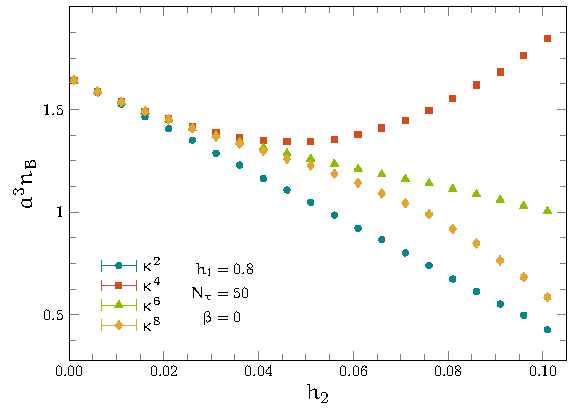
\includegraphics{convergence_numeric_kappa}
      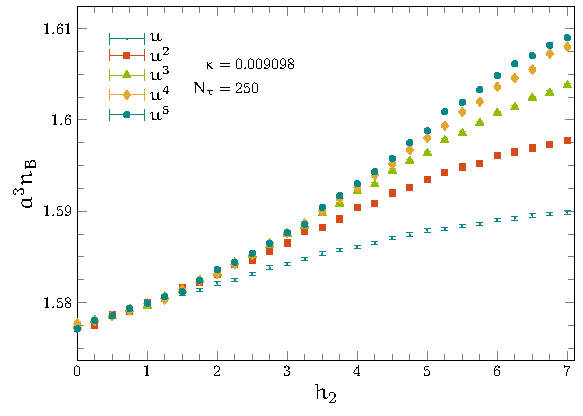
\includegraphics{convergence_numeric_beta}
    \end{adjustbox}
  \end{center}\vskip -.5cm
  \caption[
    Left: Convergence of baryon number density in lattice units as a
      function of the nearest neighbour coupling $h_2$ in various orders of the
      hopping expansion at strong coupling. Right: Corresponding convergence plot
      at different orders in the character expansion parameter $u$.
  ]{
    Left: Convergence of baryon number density in lattice units as a
    function of the nearest neighbour coupling $h_2$ in various orders of the
    hopping expansion at strong coupling. Right: Corresponding convergence plot
    at different orders in the character expansion parameter $u$.%
    \protect\footnotemark}
  \label{fig:numerical_convergence}
\end{figure}
\footnotetext{Simulation data courtesy of Mathias Neuman}
%
The simulations were carried out using both algorithms, MC with reweighting and
CL, and the results were cross checked \citep{Langelage:2014vpa}. Both methods
give compatible results within the parameter range for which the effective
theory is well defined. Our first task is to assess the range of validity of the
strong coupling, heavy quark action. One expects the additional orders in
$\kappa$ to extend the convergence region, within which the description of
thermodynamic functions by the effective action is reliable. We test this by
computing the baryon number density at fixed values of the coupling $h_1$ and
$N_{\tau}$.  Varying $\kappa$ then allows us to assess the convergence of the
expansion of the kinetic quark determinant.  \figref{fig:numerical_convergence}
(left) shows the results obtained with effective actions of increasing order in
$\kappa$. One clearly observes how two adjacent orders stay together for larger
values of $h_2(\kappa)$ as the order increase, thus extending the range where
our effective action is reliable.  \figref{fig:numerical_convergence} (right)
shows the same exercise for the largest $\kappa$ considered with the numerics, this
time increasing the orders of the character expansion. We observe good
convergence up to $\beta\sim 6$, which is a sufficiently weak coupling to allow
for continuum extrapolations. It is interesting to note that the convergence
properties are not determined by the size of the expansion parameters alone.
Even though the $u(\beta)$-values far exceed the $\kappa$-values employed in the
figures, convergence in $u(\beta)$ appears to be faster.  The gain in
convergence region by the additional orders in the effective action can be
exploited to study the systematics of our effective theory.
%

We will leave the numerical evaluation for now and will shift our focus to a
purely analytical treatment of the effective 3D theory using graphical methods
borrowed from the linked cluster formalism.

\cleardoublepage
\chapter{Analytic Evaluation of the Effective Theory} \label{chap5}

In \chapref{chap4} we introduced the dimensionally reduced effective theory for
heavy quarks at strong coupling. We ended the chapter with a section on the
numerical handling of the theory and its advantages over full lattice gauge
theory simulations. Although a lot of progress has been made evaluating the
predictions of the theory \citep{Fromm:2011qi,Fromm:2012eb,Langelage:2014vpa},
we see from the convergence plots in \figref{fig:numerical_convergence} that
convergence is slow and other approaches should be considered.

It was observed in one of the previous studies of the effective theory
\citep{Langelage:2014vpa} that it is possible to treat the effective theory
purely analytical which provides a plethora of useful methods which we will
explore in this chapter. First and foremost it lends insight into the
mathematical and physical structure of the effective theory and serves as a
cross check for the numerical methods. In \secref{sec:cluster_expansion} we will
present the linked cluster expansion which will provide the building blocks for
a systematic study of the analytic evaluation. We will see how one can translate
between the language of spin statistics and nearest neighbour systems and the
strong coupling, heavy quark formalism. In \secref{sec:analytic_resummation} we
will introduce a new resummation scheme to the analytic evaluation which is
inaccessible to numerical methods. To do this we will exploit the care we put
into the section on effective theory combinatorics.

In \secref{sec:evaluation} we will utilise the full power of the analytic
expressions to study the various aspects of the theory at hand, comparing with
numerical results, studying lattice artefacts and more.

Finally in \secrefs{sec:large_nc_study,sec:yang_lee_zeros} we carry out two
exploratory studies in which the analytic evaluation is paramount. Although
these still pose a lot of open questions, we will build foundations on which
future studies can be performed.

\section{Linked cluster expansion} \label{sec:cluster_expansion}

We start once more on a more fundamental level by introducing the linked cluster
formalism for scalar fields with nearest neighbour interactions. Although the
following section to a sense should be complete, we refer to introductory texts
on the subject for more details, e.g. \citep{Wortis:1980zb,Reisz:1995ag}, and
\citep{Domb:1980zb,Martin:1980zb} for a physics focused presentation of simple
graph theoretical practices. After the fundamentals are out of the way we study
how one can expand the formalism to also include $n$-point interactions with
finite spatial extent, a system in which the effective theory can then be
expressed.

\subsection{Classical linked cluster expansion for nearest neighbour interactions}
\label{sec:classical_lce_nn}

To introduce the framework we consider a scalar field with a $2$-point coupling
%
\begin{equation} \label{eq:scalar_field_Z}
  \mathcal{Z} = \int [\mathrm{d} \phi] e^{-S_0[\phi] + \frac{1}{2} \sum_{x,y}
    \phi(x) v(x,y) \phi(y)},
\end{equation}
%
where function $v(x,y)$ encodes the coupling information.We will assume that the
coupling strength is small enough to justify an expansion around the free
theory. To facilitate the expansion we introduce source fields $J(x)$ and define
the generating functional
%
\begin{equation}
  \mathcal{Z}[J] = \int [\mathrm{d} \phi] e^{-S[\phi] + \sum_x J(x) \phi(x)}.
\end{equation}
%
Since our goal is to study thermodynamic quantities, we shift our attention to
the computation of the grand canonical potential $\mathcal{W}$, or the generating functional
of connected correlation functions
%
\begin{equation}
  \mathcal{W}[J,v] = \log \mathcal{Z}[J,v].
\end{equation}
%
A linked cluster expansion (\emph{LCE}) of the grand canonical potential is then defined as
the Taylor expansion with respect to the coupling $v(x,y)$ around the free
theory
%
\begin{equation} \label{eq:cluster_expansion_def}
  \mathcal{W}[J,v] = \bigg( \exp \bigg(\frac{1}{2} \sum_{x,y} v(x,y)
    \frac{\delta}{\delta \hat{v}(x,y)} \bigg) \bigg) \mathcal{W}[J,\hat{v}]
    \,\Bigg|_{\hat{v}=0}.
\end{equation}
%
One can rewrite the derivative of $\mathcal{W}$ with respect to the couplings in
terms of derivatives with respect to the sources
%
\begin{equation}
  \frac{\delta \mathcal{W}}{\delta v(x,y)} = \frac{\delta^2 \mathcal{W}}{\delta
    J(x) \delta J(y)} + \frac{\delta \mathcal{W}}{\delta J(x)} \frac{\delta \mathcal{W}}{\delta J(y)}.
\end{equation}
%
We also know that $\mathcal{W}[J]$ is the generating functional of the
connected $n$-point functions 
%
\begin{equation}
  \frac{\delta \mathcal{W}}{\delta J(x)} \bigg|_{J=\mathrlap{0}} 
    = \frac{1}{\mathcal{Z}} \int [\mathrm{d} \phi] \, \phi(x) \, e^{-S[\phi]}
    \equiv \langle \phi(x) \rangle,
\end{equation}
%
which for higher order derivatives produces the cumulants
%
\begin{equation}
  \frac{\delta^2 \mathcal{W}}{\delta J(x) \delta J(y)} \bigg|_{J=\mathrlap{0}} 
    = \langle \phi(x) \phi(y) \rangle - \langle \phi(x) \rangle \langle \phi(y) \rangle.
\end{equation}
%
To second order the expansion in \meqref{eq:cluster_expansion_def} is
%
\begin{multline} \label{eq:linked_cluster_2nd_order}
  \mathcal{W}[J, v] = \mathcal{W}[J,0]
    + \frac{1}{2} \sum_{x,y} v(x,y) \frac{\delta \mathcal{W}[J,\hat{v}]}{\delta \hat{v}(x,y)} \bigg|_{\hat{v}=0} \\
    + \frac{1}{8} \sum_{x,y} \sum_{z,w} v(x,y) v(z,w) \frac{\delta^2
      \mathcal{W}[J,\hat{v}]}{\delta \hat{v}(x,y) \delta \hat{v}(z,w)}
    \bigg|_{\hat{v}=0} + \dots
\end{multline}
%
We define the coupled $n$-point functions by
%
\begin{equation}
  \mathcal{M}_n(x_1, x_2, \dots, x_n) = \frac{\delta^n \mathcal{W}[J,v]}{\delta
    J(x_1) \delta J(x_2) \cdots \delta J(x_n)}
\end{equation}
%
which in turn define the free theory $n$-point functions
%
\begin{equation}
   \mathcal{M}_n(x_1, x_2, \dots, x_n) \big|_{v = 0}
   = M_n(x_1) \delta(x_1, x_2, \dots, x_n)
\end{equation}
%
where the Kronecker deltas naturally arise in the free theory
%
\begin{equation}
  x \neq y \hskip .2cm\Rightarrow\hskip .2cm
    \langle \phi(x) \phi(y) \rangle \big|_{v=0} = \langle \phi(x) \rangle \langle \phi(y)
    \rangle.
\end{equation}
%
We can easily see from the deltas that the cluster expansion constitutes an
expansion in connected graphs as everything disconnected would give vanishing
contributions. We can rewrite the second order derivative in $v$ in 
\meqref{eq:linked_cluster_2nd_order} in terms of derivatives w.r.t. the sources,
and thus the free $n$-point functions, which gives
%
\begin{multline} \label{eq:free_energy_before_graph}
  \mathcal{W}[v] = \mathcal{W}[0] + \frac{1}{2} \sum_{x,y} M_1(x) \,v(x,y)\, M_1(y)
  + \frac{1}{4} \sum_{x,y} M_2(x) \,v^2(x,y)\, M_2(y)\\+ \frac{1}{2} \sum_{x,y,z}
  M_1(x) \,v(x,y)\, M_2(y) \,v(y,z)\, M_1(z) + \dots
\end{multline}

\subsection{Graphical definitions}

Although the coefficients for the $v^n$ term can be computed systematically from
\meqref{eq:cluster_expansion_def}  as we showed to second order in
\meqref{eq:linked_cluster_2nd_order}, the process is tedious. However there
exists a formalism in which the terms and their prefactors can be written down
immediately in an intuitive way.
%
%\theoremstyle{definition}%
\begin{definition}{Connected graph}\label{def:graph}\\
  A graph is a set of vertices and bonds where every bond connects two distinct
  vertices. An $n$-rooted graph has $n$ fixed, distinguishable, external
  vertices, while all non-rooted vertices are free. A vertex is said to be
  \emph{$n$-valent} if it has $n$ bonds attached to it.

  A connected graph has the property that one can always move from one vertex to
  another through a continuous set of movements along the graph's bonds. A graph
  which is not connected is disconnected.

  Two $n$-rooted graphs are \emph{isomorphic} if there exists a labelling of the
  bonds and vertices so that the bonds and vertices of the two graphs can be
  made identical. The number of distinct isomorphic labellings of a graph is
  called the graph's \emph{symmetry factor}.
\end{definition}
%
\noindent{}%
To compute $\mathcal{W}$ one simply takes the set of all topologically distinct
$0$-rooted connected graph. The order counting is on the bond level, meaning
that at $\mathcal{O}(v^3)$ we only take $0$-rooted connected graphs with three
or fewer bonds. The final ingredient is a rule for translating between the
graphical representation and the mathematical expression for the grand canonical
potential
%
%\theoremstyle{ruledef}%
\begin{ruledef}{Grand canonical potential $\mathcal{W}$} \label{rule:free_energy}
  \begin{enumerate}
    \item Assign a symbol, $x_1, x_2, \dots, x_n$ to every vertex
    \item To every bond connecting vertices $x_i$ and $x_j$ add a factor
      $v(x_i,x_j)$
    \item For every vertex $x_i$ with valence $p$, add a factor $M_p(x_i)$
    \item Add a sum over the entire lattice for every vertex symbol $x_i$
    \item Divide by the symmetry factor of the graph
  \end{enumerate}
\end{ruledef}
%
\noindent{}%
Using this rule we can write the grand canonical potential in
\meqref{eq:free_energy_before_graph} using a set of graphs
%
\begin{equation}
  \mathcal{W}[v] \:=\:
  \tikz[graph style] \node[skeleton node] {};
  \:+\: \textstyle\frac{1}{2}  \:
  \begin{tikzpicture}[graph style]
    \node[skeleton node] (n1) {};
    \node[skeleton node] (n2) [below=of n1] {};
    \draw[skeleton bond] (n1) -- (n2);
  \end{tikzpicture}
  \:+\: \textstyle\frac{1}{2}  \:
  \begin{tikzpicture}[graph style]
    \node[skeleton node] (n1) {};
    \node[skeleton node] (n2) [position=60 degrees from n1]  {};
    \node[skeleton node] (n3) [position=300 degrees from n2] {};
    \draw[skeleton bond] (n1) -- (n2);
    \draw[skeleton bond] (n2) -- (n3);
  \end{tikzpicture} 
  \:+ \textstyle\frac{1}{4} \:
  \begin{tikzpicture}[graph style]
    \node[skeleton node] (n1) {};
    \node[skeleton node] (n2) [below=of n1] {}
      edge[skeleton bond, bend left=45]  (n1)
      edge[skeleton bond, bend right=45] (n1);
  \end{tikzpicture}
  + \dots \,.
\end{equation}
%
The equality between \ruleref{rule:free_energy} and the grand canonical
potential LCE \meqref{eq:cluster_expansion_def} is in no way trivial and proofs
for the equality are given in e.g.  \citep{Englert:1963pr,Bloch:1965jp}. The
topology of the interaction is still yet to be specified and the sums over the
symbols \{$x_1$,\dots,$x_n$\} run over the entire lattice. Further
simplification can be achieved by choosing e.g. a uniform nearest neighbour
coupling
%
\begin{equation}
  v(x,y) = 
    \begin{cases}
      \hskip .1cm v & \text{ if $x$ and $y$ are nearest neighbours}\\
      \hskip .1cm 0 & \text{ else}.
    \end{cases}
\end{equation}
%
We have chosen nearest neighbour interactions here, although it has been shown
that a graphical expansion non nearest neighbour couplings can be reordered in
such a way that the class of graphs are identical to the nearest neighbour case
\citep{Pordt:1996it}. For nearest neighbour interactions the grand canonical
potential simplifies further
%
\begin{equation} \label{eq:free_energy_with_embedding}
  \mathcal{W}[v] = N M_0 + \frac{q}{2} v N M_1^2 + \frac{q}{4} v^2 N M_2^2
    + \frac{q^2}{2} v^2 N M_1^2 M_2 + \dots
\end{equation}
%
where $q$ is the $2 d$ for a $d$-dimensional square lattice. This factor is
called the embedding number\footnote{Also referred to as the \emph{lattice
    constant} in the lattice community} of a graph onto the lattice, and will
differ from lattice to lattice. For every graph in with a uniform nearest
neighbour interaction the sum over the symbols / coordinates will result in $N$,
the number of lattice sites, times the embedding number of the graph. Although
it might seem wrong to include all possible embeddings as e.g. the $q^2$ in the
$M_1^2 M_2$ term will natually include the embedding corresponding to the
$M_2^2$ term. This is however not a problem as the $M_n$ factors are given in
terms of commutators and applying the methods of moments and cumulants from
\secref{sec:moments_cumulants} we see that the system resolves these issues
automatically. The embedding number is dependent on the lattice, so that e.g.
the three bond graph
%
\begin{equation}
  \begin{tikzpicture}[graph style]
    \node[skeleton node] (n1) {};
    \node[skeleton node] (n2) [right=of n1] {}
      edge[skeleton bond]  (n1);
    \node[skeleton node] [position=60 degrees from n1] {}
      edge[skeleton bond] (n1)
      edge[skeleton bond] (n2);
  \end{tikzpicture}
\end{equation}
%
has an embedding number of zero on a square lattice as there is no way to
resolve the nearest neighbour requirement of \ruleref{rule:free_energy}. On a
triangular lattice on the other hand it would have a non-zero embedding number.
A table of the four bond graphs with symmetry factors and embeddings on a square
lattice can be found in \tabref{tab:graphs_embeddings}. When we later
extrapolate the graphical methods to the effective theory we will see that these
are all graphs needed to carry out a computation to order $\kappa^8$.

\begin{table}[ht]
  \begin{center}
    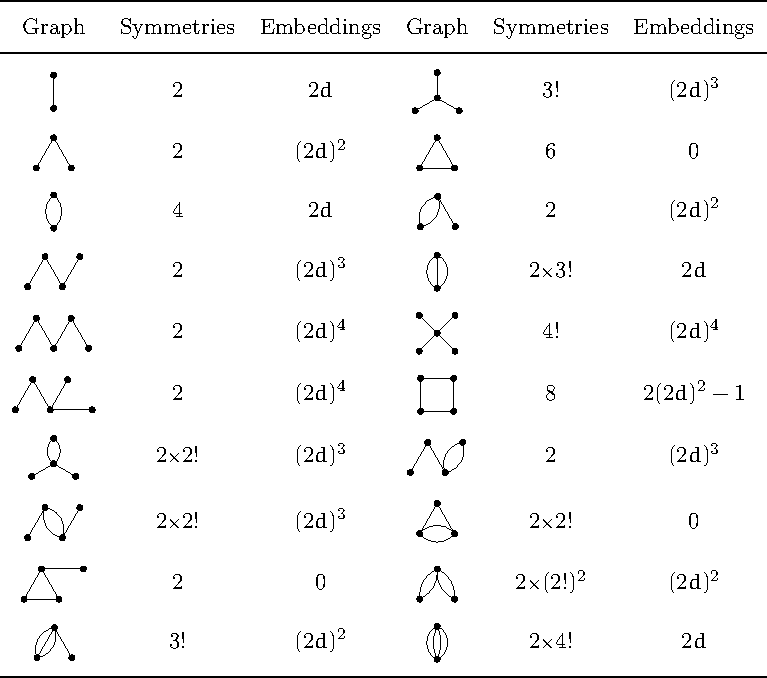
\includegraphics{embedding_and_symmetry}
  \end{center}
  \caption{Graphs with up to four bonds with symmetry factor and the embeddings
  on a $d$ dimensional square lattice.}
  \label{tab:graphs_embeddings}
\end{table}

In the next section we will see how to map the effective theory onto an LCE
framework and the additional condsiderations that has to be taken into account.

\subsection{LCE for the effective theory at LO}

We start working with the leading order action to establish corresponding
quantities in the effective action to the ones introduced in the previous
section. In the dense regime ($\mu \gg T$) the LO effective partition function
is
%
\begin{equation}
  \mathcal{Z}_2 = \int [ \mathrm{d} U ]_0 \det{}^{N_f} \qstat \exp \bigg(-
  h_2 N_f \sum_{\langle x,y \rangle} W_{11} (x) W_{11} (y) \bigg),
\end{equation}
%
as we showed in \chapref{chap4}. Comparing the above equation with the scalar
field partition function we used to introduce the LCE,
\meqref{eq:scalar_field_Z}, we see that there is a close to one-to-one
correspondence between the two systems
%
\begin{equation}
  \phi \Leftrightarrow W_{11}, \hskip .5cm v \Leftrightarrow 2 h_2 N_f, \hskip .5cm
  e^{-S_0[\phi]} \Leftrightarrow \mathcal{J} (U_0, W_{11}) \det \qstat,
\end{equation}
%
where $\mathcal{J} (U_0, W_{11})$ is the Jacobian determinant for the variable
change. There is however no need to compute $S_0[W_{11}]$ explicitly as the free
energy only depends on the $n$-point functions $M_n$, which in turn depends on
expectation values of the free theory. We define the $n$-point functions in
terms of $z$-functions, which are (for $N_f = 1$)
%
\begin{subequations}
\begin{alignat}{99}
  \centermathcell{z_{0}} &= &&\int \mathrm{d} W \det \qstat
    &&= 1 + 4 h_1^3 + h_1^6, \\
  \centermathcell{z_{(11)}} &=  &&\int \mathrm{d} W \det \qstat
    W_{11} &&= 6 h_1^3 + 3 h_1^6, \\
  \centermathcell{z_{(11)^2}} &= &&\int \mathrm{d} W \det
    \qstat W_{11}^2 &&= 4 h_1^3 + 9 h_1^6, \\
  \centermathcell{z_{(11)^3}} &= &&\int \mathrm{d} W \det
    \qstat W_{11}^3 &&= h_1^3 + 17 h_1^6 + h_1^9, \\
  \centermathcell{z_{(11)^4}} &= &&\int \mathrm{d} W \det
    \qstat W_{11}^4 &&= 21 h_1^6 + 6 h_1^9,
\end{alignat}
\end{subequations}
%
while for $N_f = 2$ they take the values
%
\begin{subequations}
\begin{alignat}{99}
  \centermathcell{z_{0}} &= &&\int \mathrm{d} W \det{}^2 \qstat \,
    &&= 1 + 20h_1^3 + 50 h_1^6 + 20 h_1^9 + h_1^{12}, \\
  \centermathcell{z_{(11)}} &=  &&\int \mathrm{d} W \det{}^2 \qstat \,
    W_{11} &&= 15 h_1^3 + 75 h_1^6 + 45 h_1^9 + 3 h_1^{12}, \\
  \centermathcell{z_{(11)^2}} &= &&\int \mathrm{d} W \det{}^2
  \qstat \, W_{11}^2 &&= 6 h_1^3 + 95 h_1^6 + 96 h_1^9 + 9 h_1^{12}, \\
  \centermathcell{z_{(11)^3}} &= &&\int \mathrm{d} W \det{}^2 
  \qstat \, W_{11}^3 &&= h_1^3 + 90 h_1^6 + 188 h_1^9 + 27 h_1^{12}, \\
  \centermathcell{z_{(11)^4}} &= &&\int \mathrm{d} W \det{}^2
  \qstat \, W_{11}^4 &&= 60 h_1^6 + 312 h_1^9 + 81 h_1^{12}.
\end{alignat}
\end{subequations}
%
The $z$'s have a fairly convoluted naming scheme. The reason for this is
that when we include more orders in the effective action we will need to
put sets of $W_{\{nm\}}$ in the integrand. The $z$'s follow the naming scheme
%
\begin{equation} \label{eq:lce_z_definition}
  z_{(n_1 m_1)^{k_1}\cdots(n_p m_p)^{k_p}} = \int \mathrm{d} W \det{}^{N_f} \qstat
  W_{n_1 m_1}^{k_1} \cdots W_{n_p m_p}^{k_p}.
\end{equation}
%
A list of all the integrated $z$'s needed to compute the results we will present
later is given in \apxref{apx:z_functions}. The $n$-point functions are then
given by
%
\begin{subequations}
\begin{align}
  M_0 &= \log z_0, \\
  M_1 &= \frac{z_{(11)}}{z_0}, \\
  M_2 &= \frac{z_{(11)^2}}{z_0} - \frac{z_{(11)}^2}{z_0^2}, \\
  M_3 &= \frac{z_{(11)^3}}{z_0} - 3 \frac{z_{(11)^2} z_{(11)}}{z_0^2} + 2 \frac{z_{(11)}^3}{z_0^3}, \\
  M_4 &= \frac{z_{(11)^4}}{z_0} - 4 \frac{z_{(11)^3} z_{(11)}}{z_0^2} - 3
  \frac{z_{(11)^2}^2}{z_0^2} + 12 \frac{z_{(11)^2} z_{(11)}^2}{z_0^3} - 6 \frac{z_{(11)}^4}{z_0^4}.
\end{align} 
\end{subequations}
%
With the full analytic result for the $\mathcal{Z}_2$ partition function at hand
we can start comparing with results from the numerical evaluation. However,
first we need to establish the observables.


\section{Observables}

We introduced the definition of the observables in \secref{sec:stat-mech}, but
just as we defined them on the lattice in \secref{sec:thermal-lattice-theory},
we have to give them in terms of the parameters we are working with. We use the
fact that  $\mathcal{W}$ is linear in volume in the thermodynamic
limit, which means that the pressure is given simply as
%
\begin{equation}
  \mathcal{P} = T \bigg( \frac{\partial}{\partial V} \log \mathcal{Z}
  \bigg)_{T\mathrlap{,z}} = \frac{T}{V}\,\mathcal{W}.
\end{equation}
%
Similarly, taking the derivative with respect to fugacity is also straight
forward, we can simplify it further using
%
\begin{equation}
  z\, \frac{\partial}{\partial z} \bigg|_{T\mathrlap{,V}} = h_1
  \frac{\partial}{\partial h_1} \bigg|_{T,V}
\end{equation}
%
which means we can define the baryon number density as
%
\begin{equation}
  n_B = \frac{1}{3} n_q = h_1 \frac{1}{3} \bigg( \frac{\partial}{\partial h_1} \frac{\mathcal{W}}{V} \bigg)_{T,V}.
\end{equation}
%
To compute the energy density $e$ we need to compute the
derivative
%
\begin{equation}
  e = T^2 \bigg( \frac{\partial}{\partial T} \frac{\log \mathcal{Z}}{V}
    \bigg)_{z,V}.
\end{equation}
%
We know that $\frac{\log \mathcal{Z}}{V}$ is volume independent, and therefore
the requirement of keeping $V$ constant is automatically fulfilled. We replace
the derivative in $T$ by a derivative in $a$, and therefore have
%
\begin{equation}
  e = -\frac{1}{N_t} \bigg( \frac{\partial}{\partial a} \frac{\mathcal{W}}{V}
    \bigg)_z.
\end{equation}
%
The derivative with respect to the lattice spacing must be handled with a bit of
care. One option is to define the derivative at constant baryon mass
%
\begin{equation}
  a \frac{\partial}{\partial a} (a m_B) = a m_B.
\end{equation}
%
We base the baryon and meson masses on the full heavy quark results from
\citep{Smit:2002introduction}, and later with the additional gauge corrections
from \citep{Langelage:2014vpa}
%
\begin{alignat}{99}
  a m_M &{}={}& \,\acosh &\bigg(1 + \frac{(M^2 - 4)(M^2 - 1)}{2M^2 - 3}\bigg) &&- 24 \kappa^2 \frac{u}{1-u},\\
  a m_B &{}={}& \log &\bigg(\frac{M^3(M^3 - 2)}{M^3 - \frac{5}{4}}\bigg) &&- 18
  \kappa^2 \frac{u}{1-u},
\end{alignat}
%
where $M = \frac{1}{2 \kappa}$. In the strong coupling limit we can use this
to determine $\frac{\partial \kappa}{\partial a}$
%
\begin{multline}
  a \frac{\partial \kappa}{\partial a} = a m_B \Big/
    \:\frac{\partial a m_B}{\partial \kappa} \\
  = \scalemath{0.9}{%
    -\frac{%
        a m_B e^{-a m_B} \big( e^{a m_B} - 8 + 4 \sqrt{4 + e^{a m_B} (e^{a m_B} - 1)} \,\big)%
      }{%
        6 \scalemath{0.8}{\times} 20^{1/3} \sqrt{4 + e^{a m_B} (e^{a m_B} - 1)}
        \big(e^{-a m_B} \big( 2 + e^{a m_B} - \sqrt{4 + e^{a m_B} (e^{a m_B} - 1)} \big) \big)^{2/3}
      }}.
\end{multline}
%
Away from strong coupling one has to define the derivative in $a$ as a
derivative in $\beta$ through the use of implicit functions
%
\begin{equation}
  a \frac{d \beta}{d a} \frac{d \kappa}{d \beta} = - a \frac{d \beta}{d a}
  \frac{\partial a m_B}{\partial \beta} \,\Big/ \:
  \frac{\partial a m_B}{\partial \kappa}.
\end{equation}
%
Assuming strong coupling for now we see that the energy density is given in
terms of the two parameters of the theory
%
\begin{equation} \label{eq:energy_dens_mid_calc}
  e =  -\frac{1}{a N_t} a\frac{\partial \kappa}{\partial a}
    \frac{\partial h_1}{\partial \kappa} \frac{\partial}{\partial h_1}
    \frac{\mathcal{W}}{V} \bigg|_z
  -\frac{1}{a N_t} a\frac{\partial \kappa}{\partial a}
    \frac{\partial h_2}{\partial \kappa} \frac{\partial}{\partial h_2}
    \frac{\mathcal{W}}{V} \bigg|_z.
\end{equation}
%
We use the fact that
%
\begin{equation}
  \frac{\partial h_1}{\partial \kappa} \bigg|_z = \frac{N_t}{\kappa} h_1
\end{equation}
%
to see that the first part of \meqref{eq:energy_dens_mid_calc} is
%
\begin{equation}
  -\frac{1}{a N_t} a\frac{\partial \kappa}{\partial a}
    \frac{\partial h_1}{\partial \kappa} \frac{\partial}{\partial h_1}
    \frac{\mathcal{W}}{V} \bigg|_z
  = - \frac{1}{a} \frac{a}{\kappa} \frac{\partial \kappa}{\partial a} h_1
  \frac{\partial}{\partial h_1} \frac{\mathcal{W}}{V}
  = -3 \frac{1}{a} \frac{a}{\kappa} \frac{\partial \kappa}{\partial a} n_B
\end{equation}
%
after inserting the definition of $n_B$. Using that to first order in $\kappa$
that $\frac{\partial \kappa}{\partial a} \sim \minus{}\kappa \frac{m_B}{3}$ we see that
this first term is somehow related to the rest energy of the system. We subtract
the energy density by this shift, the resulting quantity should give a good estimate for the
binding energy of the system at low temperatures where thermal fluctuations are
suppressed. We define the dimensionless ratio of the binding energy density to
the rest energy to be
%
\begin{equation} \label{eq:epsilon_definition}
  \epsilon = \frac{e - m_{B,\text{eff}}\, n_B}{m_{B,\text{eff}}\, n_B},
\end{equation}
%
where
%
\begin{equation}
  m_{B,\text{eff}} = -3 \frac{1}{\kappa} \frac{\partial \kappa}{\partial a}.
\end{equation}
%
\begin{figure}[t]%
  {\centering%
    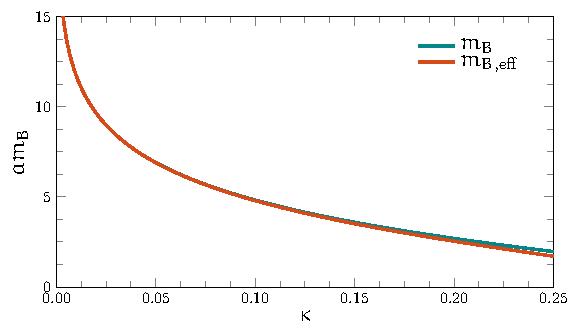
\includegraphics[width=.65\textwidth]{section_2/mb_eff_comparison}\par}
  \caption{Comparison of the effective and full baryon mass used in the definition of $\epsilon$.}%
  \label{fig:mb_eff_comparison}%
\end{figure}%
%
We plot the effective baryon mass vs the real baryon mass in the strong coupling
limit for different values of $\kappa$ in \figref{fig:mb_eff_comparison}, and
see that they mostly agree all the way to $\kappa_{\mathrm{crit}}$, which is far
enough away from the parameter range in this study that the two can be
interchanged.

In \figref{fig:convergence_cluster_Z2} we plot the baryon number density in the
strong coupling limit at varying coupling parameter $h_2$, which can be used to
test the convergence of the expansion, similar to what we did in \chapref{chap4}
with \figref{fig:numerical_convergence} (left). We see that the higher order
linked cluster contribution has a small effect on the convergence, and that it
agrees with the results from the simulations.

\begin{figure}
  \begin{center}
    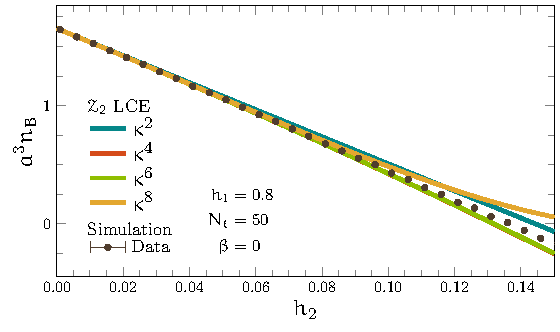
\includegraphics[width=.65\textwidth]{section_2/nb_convergence_cluster_Z2}
  \end{center}
  \caption{Convergence of LCE carried out on the LO effective theory
    $\mathcal{Z}_2$, compared to numerical data for the same parameters.}
  \label{fig:convergence_cluster_Z2}
\end{figure}

\begin{figure}
  \begin{center}
    \begin{adjustbox}{max width=\textwidth}
      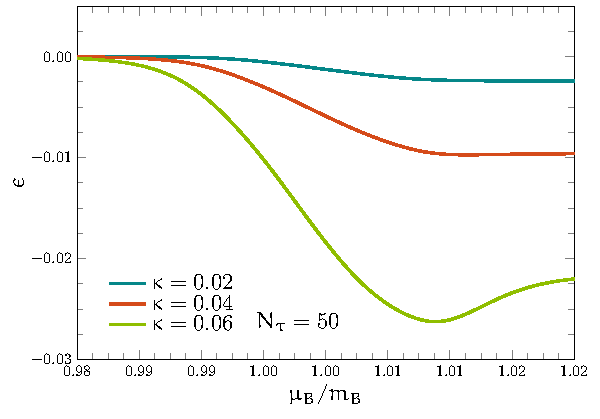
\includegraphics{section_2/binding_energy_Z2_k2}
      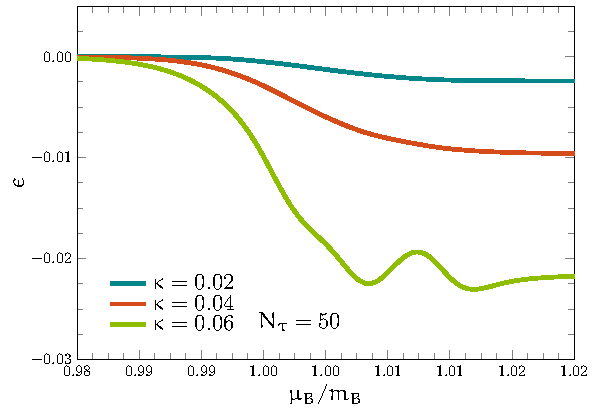
\includegraphics{section_2/binding_energy_Z2_k8}
    \end{adjustbox}
  \end{center} \vskip -.5cm
  \caption{Binding energy $\epsilon$ for three different values of $\kappa$ with
    the $\mathcal{O}(\kappa^2)$ LCE of $\mathcal{Z}_2$ on the left and with the
    $\mathcal{O}(\kappa^8)$ LCE of $\mathcal{Z}_2$ on the right.}
  \label{fig:binding_energy_Z2}
\end{figure}

At this point a note on the multi level expansions is in order. Using the
methods outlined in \chapref{chap4} we compute the effective theory to some
order in the smallness parameters $\kappa$ and $u$. This defines a unique system
with a unique action, which can then be simulated with Monte Carlo or Langevin
algorithms. Another alternative is to analyse the parition function at the given
expansion order and determine the new expansion parameters (in this case $h_2$).
A second expansion can then be carried out to evaluate this specific system
order by order in this expansion parameter. If the simulation converges to the
correct result it is expected to reproduce the full (all order) linked cluster
expansion result of the effective theory at a given order.

Finally we plot the binding energy ratio $\epsilon$ as a function of the
chemical potential for various values of $\kappa$ in
\figref{fig:binding_energy_Z2}. We see that the binding energy decrease the
constituent quark masses (increase $\kappa$), which is what one would expect.
The plot on the left is to leading order in $h_2$, while the plot on the right
shows the fourth order, $h_2^4$, of the expansion. As one can see higher order
solution develops some interesting behaviour at the higher values of $\kappa$ as
we pass the $\mu_B / m_B = 1$ line. It is however beyond convergence, and we
need more orders in the effective theory before we can say anything about the
behaviour at higher chemical potential.

\subsection{Scale setting and the continuum limit}

Up to now we have only considered observables at finite lattice spacing, and
these observables have always been computed as dimensionless ratios of these
so far unspecified lattice spacings. However for us to be able to make any
connections to other fields we first have to determine the physical scale of the
problem. As we outlined in \secref{sec:scale_setting} we need to determine the
scale generated by the regulator, $a$. One way to do this is to analyse the
static potential and link the curvature of this potential to the characteristic
length scale of QCD interactions (the so called \emph{Sommer parameter}
\citep{Sommer:1993ce}). In this way one can determine a function
$a(\beta,\kappa)$ that encodes the scale information. We assume that the heavy
quarks have little influence over the running of the coupling, and therefore for
small $\kappa$ we assume $a(\beta,\kappa) \approx a(\beta)$. We make use of the
interpolation formula for $a(\beta)$ \citep{Necco:2001xg}
%
\begin{multline}
  a = r_0 \exp (-1.6804 - 1.7331(\beta-6) + 0.7849(\beta-6)^2- 0.4428 (\beta-6)^3),\\\text{for } \beta \in [5.7, 6.29],
\end{multline}
%
using the Sommer parameter $r_0 = 0.5 \:\mathrm{fm}$. The interpolation formula
is plotted in \figref{fig:a_of_beta} (left).

\begin{figure}
  \begin{center}
    \begin{adjustbox}{max width=0.99\textwidth}
    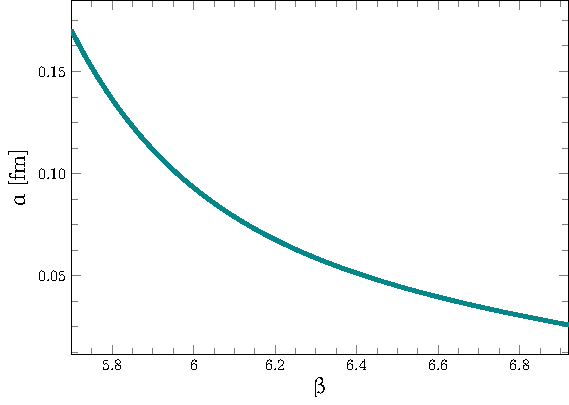
\includegraphics{section_2/a_of_beta_plot}
    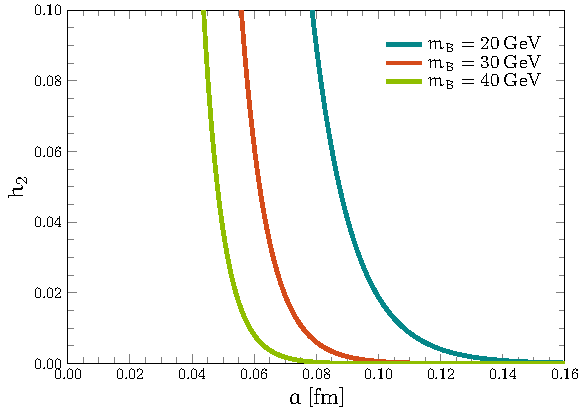
\includegraphics{section_2/h2_of_a_plot}
    \end{adjustbox}
  \end{center}\vskip -.5cm
  \caption{Left: The scale range accessible to the Necco-Sommer interpolation
    formula for strong coupling QCD. Right: The effective nearest neighbour
    coupling $h_2$ as a function of the lattice spacing keeping $m_B$ fixed at
    $T = 10 \:\mathrm{MeV}$.}
  \label{fig:a_of_beta}
\end{figure}

For the continuum limit it is important to vary the variables in such a way that
the physical system remains unchanged. Analogous to how we defined the energy
density by taking the $a$ derivative in such a way that $m_B$ remained constant,
we choose to vary the parameters $\kappa(a), \beta(a), N_t(a)$ in such a way
that $\partial_a m_B = 0$ and $\partial_a T = 0$. Some of the values at
different lattice spacings are shown in \tabref{tab:parameter_values} where we
have fixed the baryon mass to be $30 \: \mathrm{GeV}$. We observe that moving
towards the continuum limit not only decreases the constituent quark masses, but
also increase the number of temporal slices needed to fix temperature. These two
effects combine when computing the effective coupling constant $h_2 = \kappa^2
N_t / N_c$, as is clearly demonstrated in \figref{fig:a_of_beta} (right).

\begin{table}
  \begin{center}
  \begin{tabular}{cccc}
    $\beta$ & $a\hskip .1cm[\mathrm{fm}]$ & $N_t$ & $\kappa$ \\ \toprule
    $5.70$ & $0.170$ & $116$ & $0.000089$ \\
    $5.75$ & $0.152$ & $130$ & $0.000224$ \\
    $5.80$ & $0.136$ & $145$ & $0.000491$ \\
    $5.85$ & $0.123$ & $160$ & $0.000964$ \\
    $5.90$ & $0.112$ & $177$ & $0.001724$ \\
    $5.95$ & $0.102$ & $194$ & $0.002851$ \\ \bottomrule
  \end{tabular} \hskip 1cm
  \begin{tabular}{cccc}
    $\beta$ & $a\hskip .1cm[\mathrm{fm}]$ & $N_t$ & $\kappa$ \\ \toprule
    $6.00$ & $0.093$ & $212$ & $0.004419$ \\
    $6.05$ & $0.086$ & $231$ & $0.006488$ \\
    $6.10$ & $0.077$ & $250$ & $0.009100$ \\
    $6.15$ & $0.073$ & $270$ & $0.012278$ \\
    $6.20$ & $0.068$ & $291$ & $0.016030$ \\
    $6.25$ & $0.063$ & $313$ & $0.020348$ \\ \bottomrule
  \end{tabular} %
  \end{center}
  \caption{Tabulated values of the parameters of interest for the continuum
    study, computed at $T = 10 \:\mathrm{MeV}$ and $m_B = 30 \:\mathrm{GeV}$.}
  \label{tab:parameter_values}
\end{table}

Finally we demonstrate how the continuum limit is approached. We first compute
the desired observable at multiple values for $\beta$, whose upper limit is
determined my the convergence limit of our theory. E.g. the convergence plot
\figref{fig:numerical_convergence} (right) shows us that $h_2 \lesssim 0.04$ for
$\mathcal{Z}_2$ if we require no more than $10 \%$ deviation. If we then fix
$m_B = 30 \:\mathrm{GeV}$ and $T = 10 \:\mathrm{MeV}$ we find an upper limit for
$\beta \lesssim 6.02$. We then analyse the scaling of the observable with
respect to the lattice spacing
%
\begin{equation}
  O_{\mathrm{lattice}} = O_{\mathrm{continuum}} + O_1 \,a + O_2 \,a^2 +
  \mathcal{O}(a^3).
\end{equation}
%
As the expansion is based on unimproved Wilson fermions, the lattice spacing
corrections enter already at the linear level. We somewhat conservatively assume
that we still have $\mathcal{O}(a^2)$ remnants in the observables. We then fit
the observable to this function and extract the continuum limit result from
this. The fit is carried out with two sets of data points, which are chosen
depending on the observable and the value for $\mu$. A common choice here is
$\Delta \beta = 0.01$ and then use the final $10$ and $6$ points respectively
for the two fits. One then averages over the two values and take the difference
as an error estimate for the systematic error. The difference in the observable
at a fixed lattice spacing for two consecutive orders in the expansion is taken
as an error estimate which is included in the fit. The fitting procedure is
illustrated in \figref{fig:continuum_extrapolation} (left). On the right hand
side of the same figure one finds the continuum extrapolated baryon number
density for the $\mathcal{Z}_2$ partition function to the four bond LCE.

\begin{figure}
  \begin{center}
    \begin{adjustbox}{max width=\textwidth}
    \begin{tikzpicture}
      \node[inner sep=0pt] (fig1) {%
        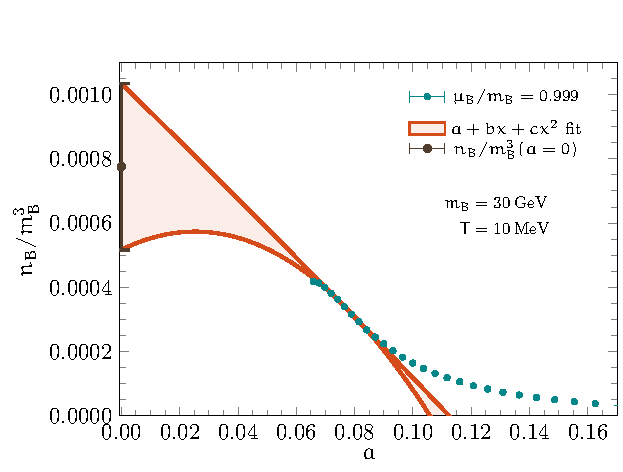
\includegraphics[trim=0 0 0 .95cm, clip]{section_2/nb_of_a_Z2}%
      };
      \node[inner sep=0pt] [right=.2cm of fig1.north east,anchor=north west] {%
        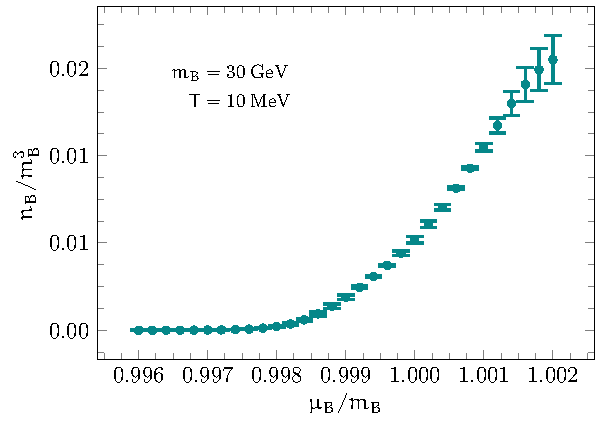
\includegraphics{section_2/nb_continuum_Z2}%
      };
    \end{tikzpicture}
    \end{adjustbox}
  \end{center}\vskip -.6cm
  \caption{Left: Plot demonstrating the continuum limit which is taken at the
    smallest accessible lattice spacing extrapolated with two different data
    sets. Right: The continuum limit of $n_B / m_B^3$ for the LO effective
    theory to four bond LCE.}
  \label{fig:continuum_extrapolation}
\end{figure}

\section{Linked cluster expansion for polymer interactions}

Before we can apply the cluster expansion formalism to the full $\mathcal{O}(u^5
\kappa8)$ effective action we need see how to handle interactions that are more
complicated than two point interactions. In this section we develop a new method
for our tool belt to handle polymer interactions with the linked cluster
formalism. We then establish the necessary mappings and apply it to the higher
order effective theories.

\subsection{Generalisation of the LCE to polymer interactions}

We start with a generalised partition function for $n$ component fields $\phi_i$
%
\begin{multline} \label{eq:multi_point_scalar_Z}
  \mathcal{Z} = \int [\mathrm{d} \phi_i] \exp \bigg(-S_0[\phi_i]
  +\frac{1}{2!} \sum_{x,y} \sum_{i,j} v_{ij}(x,y) \phi_i(x) \phi_j(y) \\
  +\frac{1}{3!} \sum_{x,y,z} \sum_{i,j,k} u_{ijk}(x,y,z) \phi_i(x) \phi_j(y)
  \phi_k(z) + \dots \bigg).
\end{multline}
%
We introduce the sources $J_i$ in a similar fashion to how they were introduced
in \secref{sec:classical_lce_nn}. This gives us a linked cluster expansion for
the grand canonical potential
%
\begin{align}
  \mathcal{W}[v,u] = \bigg[ \exp&\bigg( \frac{1}{2!} \sum_{x,y} \sum_{i,j} v_{ij}(x,y) 
    \frac{\delta}{\delta \tilde{v}_{ij}(x,y)} \bigg)  \nonumber \\
  \times\exp&\bigg( \frac{1}{3!} \sum_{x,y,z} \sum_{i,j,k} u_{ijk}(x,y,z)
    \frac{\delta}{\delta \tilde{u}_{ijk}(x,y,z)} \bigg) \cdots
    \bigg] \mathcal{W}[\tilde{v},\tilde{u}] \Bigg|_{\substack{\tilde{v}=0\\\tilde{u}=0\\\cdots}}\;.
\end{align}
%
The derivative with respect to the 3-point coupling $u$ can be expressed in
terms of derivates w.r.t. the sources
%
\begin{multline}
  \frac{\delta \mathcal{W}}{\delta u_{ijk}(x,y,z)} = \frac{\delta^3 \mathcal{W}}{\delta J_i(x) \delta J_j(y) \delta J_k(z)}
    + \frac{\delta \mathcal{W}}{\delta J_i(x)} \frac{\delta^2 \mathcal{W}}{\delta J_j(y) \delta J_k(z)}
    + \frac{\delta \mathcal{W}}{\delta J_j(y)} \frac{\delta^2 \mathcal{W}}{\delta J_i(x) \delta J_k(z)} \\
  \hspace{2cm} + \frac{\delta \mathcal{W}}{\delta J_k(z)} \frac{\delta^2 \mathcal{W}}{\delta J_i(x) \delta J_j(y)}
    + \frac{\delta \mathcal{W}}{\delta J_i(x)} \frac{\delta \mathcal{W}}{\delta J_j(y)}
    \frac{\delta \mathcal{W}}{\delta J_k(z)}\;,
\end{multline}
%
the same is also true for all the higher $n$-point interactions. To
$\mathcal{O}(v^2, u)$ (two bonds) we get
%
{\allowdisplaybreaks%
\begin{multline} 
  \mathcal{W}[v,u] = \mathcal{W}[0] + \frac{1}{2} \sum M_i(x) \,v_{ij}(x,y)\, M_j(y)
  + \frac{1}{4} \sum M_{ij}(x) \,v_{ik}(x,y)v_{jl}(x,y)\, M_{jl}(y)\\
  + \frac{1}{2} \sum M_i(x) \,v_{ij}(x,y)\, M_{jk}(y) \,v_{kl}(y,z)\, M_1(z)\\
  + \frac{1}{3!} \sum u_{ijk}(x,y,z) M_i(x) M_j(y) M_k(z) \\
  + \frac{1}{2} \sum u_{ijk}(x,y,y) M_i(x) M_{jk}(y) + \dots
\end{multline}}%
%
where the sums have been shortened for the sake of brevity and we have assumed
that the 3-point coupling is cyclic. Just as with the 2-point LCE one can
systematically carry out the lin\}ked cluster expansion, rewriting the derivatives
in the couplings $\{v, u, \dots\}$ order by order and evaluate $\mathcal{W}$.
However a graphical method is desired as it would greatly benefit the
expansion. To do this we need to further specify the geometry of the 3-point
interaction. One natural choice that is compatible with the nearest neighbour
interaction $v$ is a set of two nearest neighbour interactions
%
\begin{equation} \label{eq:udef_wedge}
  u(x,y,z) = 
    \begin{cases}
      \hskip .1cm u & \text{ if $\langle x, y \rangle$ and $\langle y, z \rangle$ are nearest neighbours},\\
      \hskip .1cm u & \text{ if $\langle x, y \rangle$ and $\langle x, z \rangle$ are nearest neighbours},\\
      \hskip .1cm u & \text{ if $\langle x, z \rangle$ and $\langle y, z \rangle$ are nearest neighbours},\\
      \hskip .1cm 0 & \text{ else},
    \end{cases}
\end{equation}
%
where we have reverted to the one-components fields for simplicity. Using this
definition for $u$, $\mathcal{W}$ evaluates to 
%
\begin{multline}
  \mathcal{W}[v,u] = N M_0 + \frac{q}{2} v N M_1^2 + \frac{q}{4} v^2 N M_2^2 \\
    + \frac{q^2}{2} v^2 N M_1^2 M_2 + \frac{q^2}{2} u N M_1^3 + \frac{q}{2} u N
    M_1 M_2 + \dots
\end{multline}
%
Graphically we can represent the above expression as
%
\begin{equation} \label{eq:lce_uv_nn}
  \mathcal{W}[v] \:=\:
  \tikz[graph style] \node[skeleton node] {};
  \:+\: \textstyle\frac{1}{2}  \:
  \begin{tikzpicture}[graph style]
    \node[inner 1] (n1) {};
    \node[inner 1] (n2) [below=of n1] {};
    \draw[bond 1] (n1) -- (n2);
  \end{tikzpicture}
  \:+\: \textstyle\frac{1}{2}  \:
  \begin{tikzpicture}[graph style]
    \node[inner 1] (n1) {};
    \node[inner 1] (n2) [right=of n1]  {};
    \node[inner 1] (n3) [position=60 degrees from n1] {};
    \node[outer 1] (n3o) at (n3) {}
      edge[bond 1] (n1)
      edge[bond 1] (n2);
  \end{tikzpicture} 
  \:+ \textstyle\frac{1}{4} \:
  \begin{tikzpicture}[graph style]
    \node[inner 1] (n1) {};
    \node[outer 1] (n1o) at (n1) {};
    \node[inner 1] (n2) [below=of n1] {};
    \node[outer 1] at (n2) {}
      edge[bond 1, bend left=45]  (n1o)
      edge[bond 1, bend right=45] (n1o);
  \end{tikzpicture}
  \:+\: \textstyle\frac{1}{2}  \:
  \begin{tikzpicture}[graph style]
    \node[inner 2] (n1) {};
    \node[inner 2] (n2) [position=60 degrees from n1]  {};
    \node[inner 2] (n3) [position=300 degrees from n2] {};
    \draw[bond 2] (n1) -- (n2);
    \draw[bond 2] (n2) -- (n3);
  \end{tikzpicture} 
  \:+ \textstyle\frac{1}{2} \:
  \begin{tikzpicture}[graph style]
    \node[inner 2] (n1) {};
    \node[inner 2] (n2) [below=of n1] {};
    \node[outer 2] at (n2) {}
      edge[bond 2, bend left=45]  (n1)
      edge[bond 2, bend right=45] (n1);
  \end{tikzpicture}
  + \dots \,.
\end{equation}
%
Where the $u$ bonds are coloured \ColBaseText{}, the $v$ bond pair is coloured
\ColHlIText{} the nodes are coloured based on the number of fields from which
interaction touches it. This is needed to distinguish e.g. the nodes in the
final term.  An alternative three point coupling could be a triangular nearest
neighbour coupling
%
\begin{equation}
  u(x,y,z) = 
    \begin{cases}
      \hskip .1cm u & \text{ if $\langle x, y \rangle$, $\langle y, z \rangle$,
                      and $\langle x, z \rangle$ are nearest neighbours},\\
      \hskip .1cm 0 & \text{ else},
    \end{cases}
\end{equation}
%
in which case the final term in \meqref{eq:lce_uv_nn} would be excluded as it is
not geometrically realisable. It would actually be better to represent this
particular version of the three point interaction with a three bond diagram
%
\begin{equation}
  \begin{tikzpicture}[graph style]
    \node[inner 2] (n1) {};
    \node[inner 2] (n2) [right=of n1] {}
      edge[bond 2]  (n1);
    \node[inner 2] [position=60 degrees from n1] {}
      edge[bond 2] (n1)
      edge[bond 2] (n2);
  \end{tikzpicture}
\end{equation}
%
as the bonds are intended to encode the nearest neighbour restriction.
Regardless of which geometry the $n$-point interactions have, there are 
numerous paths forward. One option is to compute the derivatives explicitly
order by order and sum over the coordinates explicitly. Alternatively one can
write down all mixed graphs that respect the chosen geometry and compute the
modified symmetry factor. E.g. we see that the two bond nearest neighbour graph
for the $v$ and $u$ interactions
%
\begin{equation}
  \textstyle\frac{1}{4} \:
  \begin{tikzpicture}[graph style]
    \node[inner 1] (n1) {};
    \node[outer 1] (n1o) at (n1) {};
    \node[inner 1] (n2) [below=of n1] {};
    \node[outer 1] at (n2) {}
      edge[bond 1, bend left=45]  (n1o)
      edge[bond 1, bend right=45] (n1o);
  \end{tikzpicture}, \hskip 1cm
  \textstyle\frac{1}{2} \:
  \begin{tikzpicture}[graph style]
    \node[inner 2] (n1) {};
    \node[inner 2] (n2) [below=of n1] {};
    \node[outer 2] at (n2) {}
      edge[bond 2, bend left=45]  (n1)
      edge[bond 2, bend right=45] (n1);
  \end{tikzpicture}
\end{equation}
%
have different symmetry factors due to the fact that the node relabelling
symmetry is broken. A third alternative, and the one we will focus on, is
through a second embedding step
%
\begin{ruledef}{Grand canonical potential $\mathcal{W}$ for $n$ point interactions}%
  \label{rule:free_energy_n_point}%
  \begin{enumerate}
    \item Represent the geometry of the $n$-point interaction $v_n(x_{n_1},
          x_{n_2}, \dots, x_{n_n})$ as a graph according to \defref{def:graph}
    \item Construct all graphs with the necessary number of bonds and geometry
      to the desired order, we refer to these as \emph{skeleton graphs}
    \item Embed all $n$-point interaction graphs onto the skeleton graphs
    \item For every embedded $n$-point graph that visits $x_{n_1}, x_{n_2},
      \dots, x_{n_n}$, add a factor\\ $v_n(x_{n_1}, x_{n_2}, \dots, x_{n_n})$
    \item For every vertex that with \emph{modified valence}\footnote{%
        Modified valence is the number of bonds connecting a vertex originating
        from \emph{different} $n$-point interactions} $p$, add a factor $M_p(x_i)$
    \item The correct symmetry factor will be the symmetry factor of the skeleton
          graph times the number of unique isomorphic embeddings 
  \end{enumerate}%
\end{ruledef}
%
\noindent{}%
Let us consider the embedding of a $v$-link and a $u$-"wedge" from \meqref{eq:udef_wedge}
on the three bond graph
%
\begin{equation}
  \textstyle\frac{1}{2} \:
  \begin{tikzpicture}[graph style]
    \node[skeleton node] (n1) {};
    \node[skeleton node] (n2) [position=60 degrees from n1] {}
      edge[skeleton bond, bend left=45]  (n1) 
      edge[skeleton bond, bend right=45] (n1);
    \node[skeleton node] [position=300 degrees from n2] {}
      edge[skeleton bond] (n2);
  \end{tikzpicture}
\end{equation}
%
This can be done in four different ways
%
\begin{equation}
  \textstyle\frac{1}{2} \:
  \begin{tikzpicture}[graph style]
    \node[inner 1] (n1) {};
    \node[outer 2] (n1o) at (n1) {};
    \node[inner 1] (n2) [position=60 degrees from n1] {};
    \node[outer 2] (n2o) at (n2) {}
      edge[bond 1, bend left=45]  (n1o) 
      edge[bond 2, bend right=45] (n1o);
    \node[inner 2] [position=300 degrees from n2] {}
      edge[bond 2] (n2o);
  \end{tikzpicture}
  +\textstyle\frac{1}{2} \:
  \begin{tikzpicture}[graph style]
    \node[inner 1] (n1) {};
    \node[outer 2] (n1o) at (n1) {};
    \node[inner 1] (n2) [position=60 degrees from n1] {};
    \node[outer 2] (n2o) at (n2) {}
      edge[bond 2, bend left=45]  (n1o) 
      edge[bond 1, bend right=45] (n1o);
    \node[inner 2] [position=300 degrees from n2] {}
      edge[bond 2] (n2o);
  \end{tikzpicture}
  +\textstyle\frac{1}{2} \:
  \begin{tikzpicture}[graph style]
    \node[inner 2] (n1) {};
    \node[outer 2] (n1o) at (n1) {};
    \node[inner 1] (n2) [position=60 degrees from n1] {};
    \node[outer 2] (n2o) at (n2) {}
      edge[bond 2, bend left=45]  (n1o) 
      edge[bond 2, bend right=45] (n1o);
    \node[inner 1] [position=300 degrees from n2] {}
      edge[bond 1] (n2o);
  \end{tikzpicture}
  +\textstyle\frac{1}{2} \:
  \begin{tikzpicture}[graph style]
    \node[inner 2] (n1) {};
    \node[inner 1] (n2) [position=60 degrees from n1] {};
    \node[outer 2] (n2o) at (n2) {};
    \node[outerouter 2] (n2oo) at (n2) {}
      edge[bond 2, bend left=45]  (n1) 
      edge[bond 2, bend right=45] (n1);
    \node[inner 1] [position=300 degrees from n2] {}
      edge[bond 1] (n2oo);
  \end{tikzpicture}
\end{equation}
%
where the first two are isomorphic and can be collected to one term. Hence there
are three unique embeddings of this combination onto the skeleton graph in
question, where one of the embeddings has a non-unit embedding number, and thus
a modified symmetry factor. With these two ingredients we present the
full three bond free energy
%
%\begin{multline} \label{eq:lce_uv_3b}
  \mathcal{W}[v] \:=\:
  \tikz[graph style] \node[skeleton node] {};
  \:+\: \textstyle\frac{1}{2}  \:
  \begin{tikzpicture}[graph style]
    \node[inner 1] (n1) {};
    \node[inner 1] (n2) [below=of n1] {};
    \draw[bond 1] (n1) -- (n2);
  \end{tikzpicture}
  \:+\: \textstyle\frac{1}{2}  \:
  \begin{tikzpicture}[graph style]
    \node[inner 1] (n1) {};
    \node[inner 1] (n2) [right=of n1]  {};
    \node[inner 1] (n3) [position=60 degrees from n1] {};
    \node[outer 1] (n3o) at (n3) {}
      edge[bond 1] (n1)
      edge[bond 1] (n2);
  \end{tikzpicture} 
  \:+ \textstyle\frac{1}{4} \:
  \begin{tikzpicture}[graph style]
    \node[inner 1] (n1) {};
    \node[outer 1] (n1o) at (n1) {};
    \node[inner 1] (n2) [below=of n1] {};
    \node[outer 1] at (n2) {}
      edge[bond 1, bend left=45]  (n1o)
      edge[bond 1, bend right=45] (n1o);
  \end{tikzpicture}
  \:+\: \textstyle\frac{1}{2}  \:
  \begin{tikzpicture}[graph style]
    \node[inner 2] (n1) {};
    \node[inner 2] (n2) [position=60 degrees from n1]  {};
    \node[inner 2] (n3) [position=300 degrees from n2] {};
    \draw[bond 2] (n1) -- (n2);
    \draw[bond 2] (n2) -- (n3);
  \end{tikzpicture} 
  \:+ \textstyle\frac{1}{2} \:
  \begin{tikzpicture}[graph style]
    \node[inner 2] (n1) {};
    \node[inner 2] (n2) [below=of n1] {};
    \node[outer 2] at (n2) {}
      edge[bond 2, bend left=45]  (n1)
      edge[bond 2, bend right=45] (n1);
  \end{tikzpicture}
  \:+ \textstyle\frac{1}{3!} \:
  \begin{tikzpicture}[graph style,node distance=.4]
    \node[inner 1] (n1) {};
    \node[outer 1] at (n1) {};
    \node[outerouter 1] (n1o) at (n1) {};
    \node[inner 1] (n2) [position=330 degrees from n1] {}
      edge[bond 1] (n1o);
    \node[inner 1] (n3) [position=90 degrees from n1] {}
      edge[bond 1] (n1o);
    \node[inner 1] (n4) [position=210 degrees from n1] {}
      edge[bond 1] (n1o);
  \end{tikzpicture}\\
  \:+ \textstyle\frac{1}{2} \:
  \begin{tikzpicture}[graph style]
    \node[inner 1] (n1) {};
    \node[inner 1] (n2) [position=60 degrees from n1] {};
    \node[outer 1] (n2o) at (n2) {}
      edge[bond 1] (n1);
    \node[inner 1] (n3) [position=300 degrees from n2] {};
    \node[outer 1] (n3o) at (n3) {}
      edge[bond 1] (n2o);
    \node[inner 1] (n4) [position=60 degrees from n3] {}
      edge[bond 1] (n3o);
  \end{tikzpicture}
  \:+ \textstyle\frac{1}{6} \:
  \begin{tikzpicture}[graph style]
    \node[inner 1] (n1) {};
    \node[outer 1] (n1o) at (n1) {};
    \node[inner 1] (n2) [position=60 degrees from n1] {};
    \node[outer 1] (n2o) at (n2) {}
      edge[bond 1] (n1o);
    \node[inner 1] (n3) [position=300 degrees from n2] {};
    \node[outer 1] (n3o) at (n3) {}
      edge[bond 1] (n2o)
      edge[bond 1] (n1o);
  \end{tikzpicture}
  \:+\textstyle\frac{1}{2} \:
  \begin{tikzpicture}[graph style]
    \node[inner 1] (n1) {};
    \node[inner 1] (n2) [position=60 degrees from n1] {};
    \node[outer 1] (n2o) at (n2) {};
    \node[outerouter 1] (n2oo) at (n2) {}
      edge[bond 1, bend left=45]  (n1) 
      edge[bond 1, bend right=45] (n1);
    \node[inner 1] [position=300 degrees from n2] {}
      edge[bond 1] (n2oo);
  \end{tikzpicture}
  \:+ \textstyle\frac{1}{2{\scriptstyle\times}3!} \:
  \begin{tikzpicture}[graph style]
    \node[inner 1] (n1) {};
    \node[outer 1] at (n1) {};
    \node[outerouter 1] (n1o) at (n1) {};
    \node[inner 1] (n2) [below=of n1] {};
    \node[outer 1] at (n2) {};
    \node[outerouter 1] at (n2) {}
      edge[bond 1]  (n1o)
      edge[bond 1, bend right=45] (n1o)
      edge[bond 1, bend left=45] (n1o);
  \end{tikzpicture}
  \:+ \textstyle\frac{1}{2} \:
  \begin{tikzpicture}[graph style,node distance=.4]
    \node[inner 1] (n1) {};
    \node[outer 2] (n1o) at (n1) {};
    \node[inner 2] (n2) [position=330 degrees from n1] {}
      edge[bond 2] (n1o);
    \node[inner 1] (n3) [position=90 degrees from n1] {}
      edge[bond 1] (n1o);
    \node[inner 2] (n4) [position=210 degrees from n1] {}
      edge[bond 2] (n1o);
  \end{tikzpicture} \\
  \:+ 
  \begin{tikzpicture}[graph style]
    \node[inner 2] (n1) {};
    \node[inner 2] (n2) [position=60 degrees from n1] {}
      edge[bond 2] (n1);
    \node[inner 1] (n3) [position=300 degrees from n2] {};
    \node[outer 2] (n3o) at (n3) {}
      edge[bond 2] (n2);
    \node[inner 1] (n4) [position=60 degrees from n3] {}
      edge[bond 1] (n3o);
  \end{tikzpicture}
  \:+ \textstyle\frac{1}{2} \:
  \begin{tikzpicture}[graph style]
    \node[inner 1] (n1) {};
    \node[outer 2] (n1o) at (n1) {};
    \node[inner 2] (n2) [position=60 degrees from n1] {}
      edge[bond 2] (n1o);
    \node[inner 1] (n3) [position=300 degrees from n2] {};
    \node[outer 2] (n3o) at (n3) {}
      edge[bond 2] (n2)
      edge[bond 1] (n1o);
  \end{tikzpicture}
  \:+
  \begin{tikzpicture}[graph style]
    \node[inner 1] (n1) {};
    \node[outer 2] (n1o) at (n1) {};
    \node[inner 1] (n2) [position=60 degrees from n1] {};
    \node[outer 2] (n2o) at (n2) {}
      edge[bond 2, bend left=45]  (n1o) 
      edge[bond 1, bend right=45] (n1o);
    \node[inner 2] [position=300 degrees from n2] {}
      edge[bond 2] (n2o);
  \end{tikzpicture}
  \:+\textstyle\frac{1}{2} \:
  \begin{tikzpicture}[graph style]
    \node[inner 2] (n1) {};
    \node[outer 2] (n1o) at (n1) {};
    \node[inner 1] (n2) [position=60 degrees from n1] {};
    \node[outer 2] (n2o) at (n2) {}
      edge[bond 2, bend left=45]  (n1o) 
      edge[bond 2, bend right=45] (n1o);
    \node[inner 1] [position=300 degrees from n2] {}
      edge[bond 1] (n2o);
  \end{tikzpicture}
  \:+\textstyle\frac{1}{2} \:
  \begin{tikzpicture}[graph style]
    \node[inner 2] (n1) {};
    \node[inner 1] (n2) [position=60 degrees from n1] {};
    \node[outer 2] (n2o) at (n2) {};
    \node[outerouter 2] (n2oo) at (n2) {}
      edge[bond 2, bend left=45]  (n1) 
      edge[bond 2, bend right=45] (n1);
    \node[inner 1] [position=300 degrees from n2] {}
      edge[bond 1] (n2oo);
  \end{tikzpicture}
  \:+ \textstyle\frac{1}{2} \:
  \begin{tikzpicture}[graph style]
    \node[inner 1] (n1) {};
    \node[outer 2] at (n1) {};
    \node[outerouter 2] (n1o) at (n1) {};
    \node[inner 1] (n2) [below=of n1] {};
    \node[outer 2] at (n2) {}
      edge[bond 2]  (n1o)
      edge[bond 1, bend right=45] (n1o)
      edge[bond 2, bend left=45] (n1o);
  \end{tikzpicture}
  \:+\dots\:.
\end{multline}

\begin{equation} \label{eq:lce_uv_3b}
  \tikz \node[anchor=base, baseline, minimum width=.9\textwidth, draw, minimum height=2cm, ColourHl1,thick] {Dummy equation}; 
\end{equation}

\subsection{Application to the effective theory, graph embeddings}

\begin{figure}[t]
  {\centering
    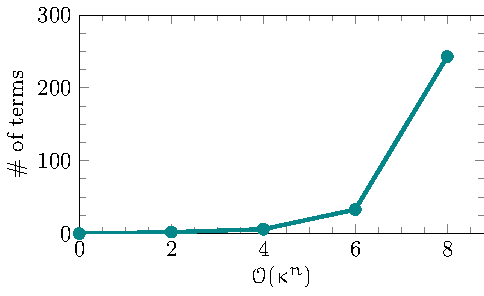
\includegraphics[width=.5\textwidth]{section_3/cluster_number_of_terms}\par}
  \caption{Number of analytic terms from the LCE of the effective theory}
  \label{fig:cluster_num_terms}
\end{figure}

Once more we will compare the effective theory partition function to the one of
the LCE and create a correspondence. We will increase the order of the effective
theory by one, working with $\mathcal{Z}_4$. The method is however easily
generalisable, and the $\mathcal{Z}_8$ effective theory partition function has
been considered for the upcoming result. The $\mathcal{O}(\kappa^4)$ partition
function is
%
\begin{multline}
  \mathcal{Z}_4 = \int [ \mathrm{d} U ]_0 \det{}^{N_f} \qstat \exp \bigg(-\frac{1}{2}
    h_2 N_f \sum_{\langle x,y \rangle} W_{11} (x) W_{11} (y)\\
  + h_2^2 N_f \sum_{\langle x,y \rangle} \sum_{\langle y,z \rangle} W_{11}(x)
    W_{21}(y) W_{11}(z)
  + h_2^2 N_f^2 \sum_{\langle x,y \rangle} W_{21}(x) W_{21}(y) \bigg).
\end{multline}
%
The correspondence is now between the two component field $\phi_i$ in the
following manner
%
\begin{equation}
  \phi_i \Leftrightarrow \big(W_{11}, W_{21}\big)_i\:, \hskip .5cm
  e^{-S_0[\phi]} \Leftrightarrow \mathcal{J} (U_0, W_{11}, W_{21}) \det \qstat
  \:.
\end{equation}
%
The two and three point interactions are given by
%
\begin{equation}
  v_{ij}(x,y) = \delta(\langle x,y \rangle)
    \begin{pmatrix}
      -2 h_2 N_f & 0 \\
      0 & 2 h_2^2 N_f^2
    \end{pmatrix}_{ij}
\end{equation}
%
and
%
\begin{align}
  u_{1jk}(x,y,z) &= 2 h_2^2 N_f 
    \begin{pmatrix}
      0 & \delta(\langle x,z \rangle) \delta(\langle y,z \rangle) \\
      \delta(\langle x,y \rangle) \delta(\langle y,z \rangle) & 0
    \end{pmatrix}_{jk} \;,\\
  u_{2jk}(x,y,z) &= 2 h_2^2 N_f  
  \begin{pmatrix}
    \delta(\langle x,y \rangle) \delta(\langle x,z \rangle) & 0 \\
    0 & \makebox[3cm][c]{$0$}
  \end{pmatrix}_{jk}\;.
\end{align}
%
At $\mathcal{Z}_6$ we see that we have to expand the set of fields to four,
$\phi_i \Leftrightarrow \big(W_{11}, W_{21}, W_{31}, W_{32}\big)_i$,
which would result in the following two point interaction matrix
%
\begin{equation}
  v_{ij}(x,y) = \delta(\langle x,y \rangle)
    \begin{pmatrix}
      -2 h_2 N_f & 0 & 0 & 0\\
      0 & 2 h_2^2 N_f^2 & 0 & 0\\
      0 & 0 & -\textstyle\frac{1}{3} h_2^3 N_f & \textstyle\frac{4}{3} h_2^3 N_f^3\\
      0 & 0 & \textstyle\frac{4}{3} h_2^3 N_f^3 & -\textstyle\frac{1}{3} h_2^3 N_f
    \end{pmatrix}_{ij},
\end{equation}
%
and the other $n$-point functions are too long to list. The computation of the
analytic formula for $\mathcal{W}$ was carried out using all three methods
outlined above (carrying out derivatives, computing graphs directly as well as
using the embedding method). This was done to guarantee correctness of the
result. The number of terms contributing to the analytic function describing
$\mathcal{Z}_{\mathrm{QCD}}$ at a given order in our expansion scheme is plotted
in \figref{fig:cluster_num_terms}, and once more we see that the number of terms
grow exponentially as one increase the order. This necessitates the development
of software to carry out graphical combinatorics to push this to higher orders.
This would e.g. be similar to the work of L\"{u}scher and Weisz in the
groundbreaking work on the $\lambda \phi^4$ lattice theory \citep{Luscher:1988gk,Luscher:1988uq}
where they carried out a LCE to $14$\textsuperscript{th} order to show the
triviality of the theory. One should however note the added difficulty due to
the additional polymer interaction and their geometry. For example the four bond
LCE on a square lattice gives $17$ graphs, while our effective theory has $243$
graphs at the four bond level.

\subsection{Results} \label{sec:cluster_results}

We are now in a position to evaluate thermodynamic functions completely
analytically. Using the LCE we have computed the grand canonical partition
function in the thermodynamic limit though $\kappa^8 u^5$ to first order in
$N_t^{-1}$. We first compare the convergence of the theory in the two parameters
to that obtained through simulating the effective theory. The convergence in the
nearest neighbour effective coupling, $h_2$, is shown in
\figref{fig:analytic_convergeance} (left). Making a comparison to
\figref{fig:numerical_convergence} (left) we see that the analytic convergence
range matches that of the simulated data and shows good quantitative agreement.
In \figref{fig:analytic_convergeance} (right) we see the corresponding
convergence plot in the strong coupling parameter $\beta$. We see that the
analytic computation underestimates the strong coupling contributions. One
should however note the axis scales and note that the finite coupling
corrections are much smaller than the corrections in $\kappa$ and that the main
contribution of finite $\beta$ comes indirectly through a rescaling of the
system.

\begin{figure}
  \begin{center}
    \begin{adjustbox}{max width=\textwidth}
      \includegraphics{section_3/nb_of_h2_beta0}
      \includegraphics{section_3/nb_of_beta}
    \end{adjustbox}
  \end{center}\vskip -.6cm
  \caption{Convergence of the analytic expressions in $h_2$ (left) and $\beta$
    (right) overlayed with the simulation results at highest order. The
    normalised baryon number density has been used in the rightmost plot.}
  \label{fig:analytic_convergeance}
\end{figure}

Next we explore the convergence properties of the theory as we move towards
lighter quarks and smaller lattice sizes. In \figref{fig:convergence_in_spacing}
we plot the baryon number density at lower and lower lattice sizes. The error
bars are estimates of the systematic error given as the difference between two
subsequent orders in the expansion. The first observation is that at
conservative quark masses of $\sim 10 \:\mathrm{GeV}$ we see that the continuum
extrapolation is limited by extrapolation from data taken at $\sim 0.07
\:\mathrm{fm}$. However, we note that in all cases the convergence improves at
higher orders of the expansion, demonstrating the stability of the expansion.
The second observation one can make is that convergence is worse at higher
chemical potential. This combined with the fact that the slope increases makes
accessing the denser systems more difficult. This is a manifestation of fermion
saturation on the lattice, as was discussed in \secref{sec:saturation}.

\begin{figure}[t]
  \begin{center}
    \includegraphics[width=.65\textwidth]{section_3/nb_of_a_mu0999}
  \end{center} \vskip -.5cm
  \caption{Convergence of the baryon number density at smaller and smaller
    lattice spacings. Shows similar limitations to the extrapolation plot of the
  $\mathcal{Z}_2$ theory in \protect\figref{fig:continuum_extrapolation} (left).}\vskip -.2cm
  \label{fig:convergence_in_spacing}
\end{figure}

\begin{figure}
  \begin{center}
    \begin{adjustbox}{max width=\textwidth}
      \includegraphics{section_3/nb_of_mpi_a02}
      \includegraphics{section_3/nb_of_mpi_a01}
    \end{adjustbox}
  \end{center}\vskip -.6cm
  \caption{Order by order convergence as a function of the meson mass of the
    system exposing the heavy quark limits of the system. Left plot at $T = 20\:
    \mathrm{MeV}$ and $a = 0.2\:\mathrm{fm}$, right plot at at $T = 10\:
    \mathrm{MeV}$ and $a = 0.1\:\mathrm{fm}$.}
  \label{fig:convergence_mpi}
\end{figure}

In \figref{fig:convergence_mpi} we plot the convergence of the different orders
of the expansion at varying meson mass at fixed temperature and lattice
spacing. This plot demonstrates the difficulty for the effective theory to reach
smaller quark masses. Although the higher orders does indeed help with the
convergence, we see that the effect of two more orders is small compared to the
relevant scales of the problem. We can therefore not picture an extension to
smaller quark masses through brute force order by order computations.

\subsection{Pad\'e approximants}

An alternative, but very powerful tool for series analyses is the \emph{Pad\'e
approximants}. It is simply a reordering of the power series into a rational
expression
%
\begin{equation}
  [L/M](z) = \frac{a_0 + a_1 z + \dots + a_L z^L}{b_0 + b_1 z + \dots + b_M
    z^M},
\end{equation}
%
so that it's Maclaurin series agrees with the original series to
$(L+M)$\textsuperscript{th} order
%
\begin{equation}
  \sum_{i = 0}^{\mathclap{L+M}} c_i z_i = [L/M](z) + \mathcal{O}(z^{L+M+1}).
\end{equation}
%
An extensive introduction to Pad\'e approximants, their uses and properties
can be found in \citep{Baker:1996cup}. If the approximants are well defined,
they tend to show better convergence properties than their corresponding
Maclaurin series. If one considers a long enough series it is also possible to
use the Pad\'{e} formulation to analyse critical points and non analyticities of
the theory. However one should be careful as the Pad\'{e} series will pick up
both the real physical singularities as well as artefact singularities due to
the fractional nature of the expression. To resolve this one can e.g. study the
different Pad\'e approximants as the $L$-$M$ ratio is a sliding scale. It is
however known that the diagonals ($[L/L]$ and $[L-1/L]$) possess various
favourable properties
\citep[and references therein]{Gaunt:1980zb,Guttmann:1989zb}.

In our case the Pad\'e variable is $h_2$, and the highest order is $L+M = 4$.
After discarding the approximants with artificial singularities we can
compare the convergence to that of the Maclaurin series. This is shown in
\figref{fig:pade_results} (left) where we once more have used the baryon number
density to investigate convergence. We see that the order by order convergence
rate of the Pad\'e approximants are far superior to those of the pure linked
cluster expansion, as is expected. 

\begin{figure}
  \begin{center}
    \begin{adjustbox}{max width=\textwidth}
      \includegraphics{section_3/nb_of_h2_pade}
      \includegraphics{section_3/binding_energy_pade}
    \end{adjustbox}
  \end{center}\vskip -.6cm
  \caption{Results from the Pad\'e approximants. Left: Convergence plot at
    strong coupling compared to the normal series from the LCE. Right: The
    nucleon binding energy as a function of chemical potential at different
    orders.}
  \label{fig:pade_results}
\end{figure}

Finally we plot the binding energy per nucleon, $\epsilon$, as defined
in \meqref{eq:epsilon_definition} with the Pad\'e series in
\figref{fig:pade_results} (right). We observe that this quantity displays the
\emph{silver blaze}, namely that it is zero up until onset transition, where it
in this case becomes negative, as was seen in \citep{Langelage:2014vpa}. With
the fourth order Pad\'e, we can extend the study to higher densities. Although
the quantitative convergence breaks down shortly after the onset transition near
$\mu_B \approx m_B$, we see new qualitative behaviour. In the higher orders we
see that the binding has a minimum and reaches a positive value at growing
chemical potential as is expected from nuclear physics. This means that we have
a qualitative bulk nuclear density, whose qualitative value is still unsettled
by the present study.

We will refrain from analysing any more results until we have introduced a final
improvement to the analytic approach.

\section{Analytic resummation} \label{sec:analytic_resummation}

So far we have managed to analytically calculate the grand canonical potential
of the effective theory to the same order as the effective theory itself, and
consequently achieved access to the thermodynamic quantities analytically.
Although this by itself is both useful due to the permanence of the results, as
well as the additional mathematical insight into the theory it admits, we have
merely reproduced the simulated results. In this section, further improvements to
the theory will be analysed, which will push the analytic evaluation beyond that
of the numerically obtained ones. We will start by introducing a resummation
scheme on the level of the effective theory first in
\secref{sec:chain_resummation}. We will then proceed to a resummation on the
cluster expansion level in \secref{sec:cluster_resummation}. Finally, in
\secref{sec:ladder_resummation}, we will review a second hypothetical
resummation, again on the level of the effective theory.

\subsection{Chain resummation} \label{sec:chain_resummation}

We start with a motivating example. Consider the following four terms from the
effective action \meqref{eq:effective_action_kapp8}
%
\begin{equation}
  h_2 N_f \sum_{\mathrm{dof}} \;
  \begin{tikzpicture}[eft graph, node distance=.4]
    \node[eft node] (n1) {1};
    \node[eft node] (n2) [below=of n1] {1}
      edge[eft bond] (n1);
  \end{tikzpicture}, \;
  - h_2^2 N_f\sum_{\mathrm{dof}}  \:
  \begin{tikzpicture}[eft graph]
    \node[eft node] (n1) {1};
    \node[eft node] (n2) [position=60 degrees from n1] {1}
      edge[eft bond] (n1);
    \node[eft node] (n3) [position=300 degrees from n2] {1}
      edge[eft bond] (n2);
  \end{tikzpicture}, \;
  h_2^3 N_f\sum_{\mathrm{dof}} \:
  \begin{tikzpicture}[eft graph]
    \node[eft node] (n1) {1};
    \node[eft node] (n2) [position=60 degrees from n1] {1}
      edge[eft bond] (n1);
    \node[eft node] (n3) [position=300 degrees from n2] {1}
      edge[eft bond] (n2);
    \node[eft node] (n4) [position=60 degrees from n3] {1}
      edge[eft bond] (n3);
  \end{tikzpicture}, \;
  - h_2^4 N_f\sum_{\mathrm{dof}} \:
  \begin{tikzpicture}[eft graph]
    \node[eft node] (n1) {1};
    \node[eft node] (n2) [position=60 degrees from n1] {1}
      edge[eft bond] (n1);
    \node[eft node] (n3) [position=300 degrees from n2] {1}
    edge[eft bond] (n2);
    \node[eft node] (n4) [position=60 degrees from n3] {1}
      edge[eft bond] (n3);
    \node[eft node] (n5) [position=300 degrees from n4] {1}
      edge[eft bond] (n4);
  \end{tikzpicture} .
\end{equation}
%
It is clear that these four terms follow a common pattern that generates a
chain. Each of the terms above extend the chain by one node while maintaining a
common prefactor. By studying the mathematically equivalent formulation, we
observe that every new link in the chain contributes a factor $h_2 W_{21}$ to
the term, in addition to the necessary spatial geometry. One can check the other
terms in the $\kappa^8$ action, e.g.
%
\begin{equation}
  2 h_2^3 N_f^2 \sum_{\mathrm{dof}} \; \Bigg(
  \begin{tikzpicture}[eft graph]
    \node[eft node] (n1) {1};
    \node[eft node] (n2) [position=60 degrees from n1] {1}
      edge[eft bond, bend left=30]  (n1)
      edge[eft bond, bend right=30] (n1);
    \node[eft node] (n3) [position=300 degrees from n2] {1}
      edge[eft bond] (n2);
  \end{tikzpicture} - 
  \begin{tikzpicture}[eft graph]
    \node[eft node] (n1) {1};
    \node[eft node] (n2) [position=60 degrees from n1] {2}
      edge[eft bond, bend left=30]  (n1)
      edge[eft bond, bend right=30] (n1);
    \node[eft node] (n3) [position=300 degrees from n2] {1}
      edge[eft bond] (n2);
  \end{tikzpicture} \Bigg), \;
  -2 h_2^4 N_f^2 \sum_{\mathrm{dof}} \; \Bigg(
  \begin{tikzpicture}[eft graph]
    \node[eft node] (n1) {1};
    \node[eft node] (n2) [position=60 degrees from n1] {1}
      edge[eft bond, bend left=30]  (n1)
      edge[eft bond, bend right=30] (n1);
    \node[eft node] (n3) [position=300 degrees from n2] {1}
      edge[eft bond] (n2);
    \node[eft node] (n4) [position=60 degrees from n3] {1}
      edge[eft bond] (n3);
  \end{tikzpicture} - 
  \begin{tikzpicture}[eft graph]
    \node[eft node] (n1) {1};
    \node[eft node] (n2) [position=60 degrees from n1] {2}
      edge[eft bond, bend left=30]  (n1)
      edge[eft bond, bend right=30] (n1);
    \node[eft node] (n3) [position=300 degrees from n2] {1}
      edge[eft bond] (n2);
    \node[eft node] (n4) [position=60 degrees from n3] {1}
      edge[eft bond] (n3);
  \end{tikzpicture} \Bigg),
\end{equation}
%
all follow the this pattern. The conjecture is then that every singly connected
node, namely every factor $W_{11}$, can be extended to a chain of arbitrary
length, and that these terms will appear in a predictable form at higher orders.
The chain resummation can schematically be represented as
%
\begin{equation} \label{eq:chain_schematic}
  \tikz[midtikz] \node[inner sep=0pt] (fig) {\includegraphics[scale=1.05]{resummation_schematic}};\;,
\end{equation}
%
in which $\mathcal{C}_0$ represents and arbitrary unsummed term with $m$ singly
connected nodes (\emph{open ends}), and $\mathcal{C}_n$ represents the same term
where the $m$ opens ends have been extended a combined total of $n$ times. We
then sum over the extension $n$ of the $m$ open ends which will result in a
replacement of all open ends
%
\begin{equation} \label{eq:chain_subst}
  W_{11}(x) \to W_{11}(x) \sum_{n=0}^{\infty} \mathcal{G}(\{x_n\}) \prod_{i=1}^{n} (-h_2) W_{21}(x_i).
\end{equation}
%
The factor $\mathcal{G}(\{x_n\})$ represents the geometry of the chain, which we
will later embed onto the polymer linked cluster expansion developed in the
previous section. Before this point we need to review the mathematical structure
of the resummation, and its origin.

\subsubsection{Combinatorial analysis}

We already introduced the combinatorics of the cold and dense regime in
\secref{sec:combinatorics}, which we will build upon in this section. The first
observation we need to make is the types of terms before the spatial gauge link
integrals that contribute to the chain. We will simply state the general pattern
here and prove it later. We define an \emph{open end} to consist of two
consecutive hops that form a pair, such as $1 \, 1$. When we introduced the
pairing notation we used the sixth order single trace as an example, which can
appear in three combinations (as in \meqref{eq:pmpmpm_pairing})
%
\begin{equation}
  \tr \tikz[baseline=-3pt] \matrix [matrix of math nodes,inner sep=1.5pt,ampersand replacement=\&]
    {1 \& 1 \& 2 \& 2 \& 3 \& 3 \\};, \hskip.5cm
  \tr \tikz[baseline=-3pt] \matrix [matrix of math nodes,inner sep=1.5pt,ampersand replacement=\&]
    {1 \& 2 \& 3 \& 3 \& 2 \& 1 \\};, \hskip.5cm
  \tr \tikz[baseline=-3pt] \matrix [matrix of math nodes,inner sep=1.5pt,ampersand replacement=\&]
    {1 \& 2 \& 3 \& 1 \& 2 \& 3 \\};.
\end{equation}
%
The first term has three open ends, the second has two open ends (including cyclic
permutations), while the final term has no open ends. An extension of the chain
is obtained by inserting a new pair in between an already existing open end.
Instead of the quark hopping forth and then directly back again, it will take a
detour through this new position
%
% TODO: Check notation consistency (positions)
\begin{subequations}
  \begin{align}
    \dots
    \tikz[baseline=-3pt]
      \matrix [matrix of math nodes,inner sep=1.5pt,ampersand replacement=\&] {1 \& 1 \\};
    \hspace{.25cm}
    &\tikz
      \draw[->,>=stealth] (0,0) -- +(1cm,0); \hspace{.3cm}
    \dots \: W_{11}(\vec{x}), \\
    \dots
    \tikz[baseline=-3pt]
      \matrix [matrix of math nodes,inner sep=1.5pt,ampersand replacement=\&] {1 \& 2 \& 2 \& 1 \\};
    \hspace{.25cm}
    &\tikz
      \draw[->,>=stealth] (0,0) -- +(1cm,0); \hspace{.3cm}
    \dots \: W_{21}(\vec{x}) W_{11}(\vec{x} + i), \\
    \dots
    \tikz[baseline=-3pt]
      \matrix [matrix of math nodes,inner sep=1.5pt,ampersand replacement=\&] {1 \& 2 \& 3 \& 3\& 2 \& 1 \\};
    \hspace{.25cm}
    &\tikz
      \draw[->,>=stealth] (0,0) -- +(1cm,0); \hspace{.3cm}
    \dots \: W_{21}(\vec{x}) W_{21}(\vec{x} + i) W_{11}(\vec{x} + i + j).
  \end{align}
\end{subequations}
%
The prefactors of terms in this resummation can be calculated from symmetry
arguments.  Assume that we know the symmetry prefactor $1/g$ of a term with $N$
open ends.  Extending one of these can be done in $N/g$ distinct ways, which all
break the previous symmetry. The sum of all such insertions thus have a
prefactor of $N/g$ which is $N$ times that of the base diagram.
However, instead of counting the number of these permutations, one can make the
observation that the problem is equivalent to distributing $n$ indistinguishable
objects to $N$ distinguishable bins. This is assuming that extending any of the
chains give the same result. This is obviously not true in general, as they
result in different geometric objects, however, when we later embed these
objects onto the linked cluster expansion we will only consider the embeddings
in which this discrepancy is irrelevant. In this special case the new symmetry
factor from extending a graph with a symmetry factor $1/g$ with $N$ open ends by
$n$ links is
%
\begin{equation} \label{eq:resummed_symmetry}
  \frac{1}{g'} = \frac{1}{g} \binom{N - 1 + n}{n}\;.
\end{equation}
%
% TODO: Reformulate
This is also only true if we consider a \emph{root graph}, which is any graph
that does not appear as an extension to any other lower order graph. This is
however not a problem as long as we carry out the resummation on an order by
order basis. With this in place we will carry out the gauge integrals
recursively on a chain matrix to show that the above mentioned expression does
indeed appear. As argued, the chain can be expressed as
%
\begin{equation}
  \tikz[baseline=-3pt]
    \matrix [
      matrix of math nodes,
      inner sep=1.5pt,
      ampersand replacement=\&
    ] {X \& 1 \& 2 \& 3 \& 4 \& \dots \& n \& n \& \dots \& 4 \& 3 \& 2 \& 1 \\};,
\end{equation}
%
where $X$ represents the remainder of the term, which may or may not include
additional open ends, and or chains. Since the expression has a recursive
structure it is natural to define the matrices $G_n$ so that
%
\begin{equation}
  \begin{tikzpicture}[baseline={([yshift=-.65ex] nodes.center)}]
    \matrix (nodes) [
      matrix of math nodes,
      inner sep=1.5pt,
      ampersand replacement=\&
    ] {1 \& 2 \& 3 \& 4 \& \dots \& n \& n \& \dots \& 4 \& 3 \& 2 \& 1 \\};
    \draw [
      decorate,
      line width=1.4pt,
      decoration={
        brace,
        mirror,
        amplitude=5pt
      },
    ]
      ([yshift=-.2cm]nodes-1-1.south west) -- ([yshift=-.2cm]nodes-1-12.south east)
      node[midway,below=5pt] {$G_n$};
    \draw [
      decorate,
      line width=1.4pt,
      decoration={
        brace,
        amplitude=5pt
      },
    ]
      ([yshift=.2cm]nodes-1-2.north west) -- ([yshift=.2cm]nodes-1-11.north east)
      node[midway,above=5pt] {$G_{n-1}$};
    \draw [
      decorate,
      line width=1.4pt,
      decoration={
        brace,
        mirror,
        amplitude=5pt
      },
    ]
      ([yshift=-1.1cm]nodes-1-3.south west) -- ([yshift=-1.1cm]nodes-1-10.south east)
      node[midway,below=5pt] {$G_{n-2}$};
  \end{tikzpicture}\; .
\end{equation}
%
The matrix $G_n$ is then defined in terms of $G_{n-1}$. In
\secref{sec:combinatorics} we saw that the static propagator in the cold dense
limit had the approximate expression \meqref{eq:leading_order_static_prop},
meaning that the effecitve hopping matrices take the form
%
\begin{alignat}{99}
  P^{ab}_{\alpha\beta}(y,x) &= \kappa \Big(\frac{1+\gamma_0}{2}\Big)_{\alpha\gamma} K^{ac}_{\vec{x}}(t_y,t_x)
    \sum_{i=1}^3  (1+\gamma_i)_{\gamma\beta} U_{\vec{x},i}^{cb} &&\delta_{\vec{y},\vec{x}+i} \\
  M^{ab}_{\alpha\beta}(y,x) &= \kappa \Big(\frac{1+\gamma_0}{2}\Big)_{\alpha\gamma} K^{ac}_{\vec{x}}(t_y,t_x)
    \sum_{i=1}^3  (1-\gamma_i)_{\gamma\beta} U^{\dagger,cb}_{\vec{x},i} &&\delta_{\vec{y},\vec{x}-i}
\end{alignat}
%
where we have shortened the $K^+$ notation for the brevity. Colour indices are
denoted by Roman characters, while the Driac indices are symbolised by Greek
letters. We also saw in \secref{sec:dirac_indices} that the Dirac trace is
somewhat trivial. The colour matrix content that enters the integrals is thus
%
\begin{equation}
  K^{ac}_{\vec{x}}(t_y,t_x) U^{cb}_{\vec{x},i}, \hskip.5cm\text{and}\hskip.5cm
  K^{ac}_{\vec{x}}(t_y,t_x) U^{\dagger{}, cb}_{\vec{x},i}.
\end{equation}
%
We are now ready to evaluate the colour integrals over the matrix $G_n$
%
\begin{align}
  G_{n}^{af}(t_1,t_2;\vec{x}_0) &= 2 \kappa^2 \sum_{i_0,t_3} \int \mathrm{d} U_{\vec{x}_0,i_0}(t_2) \;
    K_{\vec{x}_0}^{ab}(t_1,t_2)U_{\vec{x}_0,i_0}^{bc}(t_2) \nonumber \\
    &\hspace{3cm}\times G_{n-1}^{cd}(t_2,t_3;\vec{x}_0+i_0) K^{de}_{\vec{x}_0+i_0}(t_3,t_2)
    U_{\vec{x}_0,i_0}^{\dagger,ef}(t_2) \nonumber\\
  &= \frac{2 \kappa^2}{N_c} \sum_{i_0,t_3} K_{\vec{x}_0}^{ab}(t_1,t_2) G_{n-1}^{cd}(t_2,t_3;\vec{x}_0+i)
    K^{de}_{\vec{x}_0+i}(t_3,t_2) \delta_{ce}\delta_{bf} \nonumber\\
  &= \frac{2 \kappa^2}{N_c} \sum_{i_0,t_3} K_{\vec{x}_0}^{af}(t_1,t_2) \tr_c \big[ G_{n-1}(t_2,t_3;\vec{x}_0+i)
    K_{\vec{x}_0+i}(t_3,t_2) \big] \;.\label{eq:chain_integral}
\end{align}
%
The coordinate $\vec{x}_0$ is the coordinate of the beginning of the chain, and
we see that we have a recursive structure for these spatial positions as we move
on the chain $\vec{x}_{m+1} = \vec{x}_m + i_m$. We use the above equation to
define $G_{n-1}$ in terms of $G_{n-2}$
%
\begin{equation}
  G_{n-1}^{ab}(t_2,t_3;\vec{x}_1) = \frac{2 \kappa^2}{N_c} \sum_{i_1,t_4} K_{\vec{x}_1}^{ab}(t_2,t_3)
    \tr_c \big[ G_{n-2}(t_3,t_4;\vec{x}_2) K_{\vec{x}_2}(t_4,t_3) \big]\;.
\end{equation}
%
We insert the expression for $G_{n-1}$ into the one for $G_n$, and get
%
\begin{multline}
  G_{n}^{af}(t_1,t_2;\vec{x}_0)
    = \bigg(\frac{2 \kappa^2}{N_c}\bigg)^2
      \sum_{t_3,t_4} \sum_{i_0,i_1} K_{\vec{x}_0}^{af}(t_1,t_2)
      \tr_c \big[ G_{n-2}(t_3,t_4;\vec{x}_2) K_{\vec{x}_2}(t_4,t_3) \big] \\
  \times
  \begin{tikzpicture}[baseline={([yshift=-.5ex] trace.center)}]
    \node[inner sep=0pt] (trace) {%
      $\tr_c \big[ K_{\vec{x}_1}(t_2,t_3) K_{\vec{x}_1}(t_3,t_2)\big]$};
    \draw [
      decorate,
      line width=1.4pt,
      decoration={
        brace,
        mirror,
        amplitude=5pt
      },
    ]
      ([yshift=-.2cm]trace.south west) -- ([yshift=-.2cm]trace.south east)
      node[midway,below=5pt] {$-\frac{1}{2}\,W_{21}(\vec{x}_1)$};
  \end{tikzpicture} \,.
\end{multline}
%
We see that the structure of $G_{n}$ stays the same after one step of the
recursion, except for a factor of $W_{21}$ as well as sums over new degrees of
freedom. The recursion ends at $G_1$, which is the open end of the chain, and is
given by a consecutive, paired hop
%
\begin{align}
  G_{1}^{ae}(\tau_1,\tau_2;\vec{x}_n) &=
    2 \kappa^2 \sum_{i_n} \int \mathrm{d} \vec{U}_{\vec{x}_n,i_n} \, K^{ab}_{\vec{x}_n}(t_1,t_2)
    U_{\vec{x}_n,i_n}^{bc}(t_2) K^{cd}_{\vec{x}_{n+1}}(t_2,t_2)
    U_{\vec{x}_n,i_n}^{\dagger,de}(t_2) \nonumber \\
  &= \frac{2 \kappa^2}{N_c} \sum_{i_n}K^{ae}_{\vec{x}_n}(t_1,t_2)
  \begin{tikzpicture}[baseline={([yshift=-.5ex] trace.center)}]
    \node[inner sep=0pt] (trace) {%
      $\tr_c \big[ K_{\vec{x}_{n+1}}(t_2,t_2) \big]$};
    \draw [
      decorate,
      line width=1.4pt,
      decoration={
        brace,
        mirror,
        amplitude=5pt
      },
    ]
      ([yshift=-.2cm]trace.south west) -- ([yshift=-.2cm]trace.south east)
      node[midway,below=5pt] {$\frac{1}{2} W_{11}(\vec{x}_{n+1})$};
  \end{tikzpicture} \,. \label{eq:g1_integrated}
\end{align}
%
Recursively inserting the expressions for the $G_{m}$ matrices we obtain a final
result for the full chain matrix
%
\begin{multline}
  G_{n}^{ab}(t_1,t_2;\vec{x}_0) =
    K_{\vec{x}_0}^{ab}(t_1,t_2) \bigg(\frac{2 \kappa^2}{N_c}\bigg)^n
    \sum_{\substack{t_3,t_4,\\\dots,t_{n+1}}}
    \sum_{\substack{i_0,i_1,\\\dots,i_n}}
      W_{11}(\vec{x}_{n+1}) \prod_{k=2}^{n} \big(-W_{21}(\vec{x}_k)\big) \\
  =K_{\vec{x}_0}^{ab}(t_1,t_2) \bigg(\frac{2 \kappa^2}{N_c}\bigg)^n 
  N_{t}^{n-1} \sum_{\substack{i_0,i_1,\\\dots,i_n}}
    W_{11}(\vec{x}_{n+1}) \prod_{k=2}^{n} \big(-W_{21}(\vec{x}_k)\big)\;. \label{eq:full_gn}
\end{multline}
%
The sums over the temporal variables could be trivially evaluated as the
$W_{nm}$ factors are independent of their time argument.

To tie it all together let us consider a generic contribution which has $N$ open
ends
%
\begin{equation} \label{eq:chain_begin}
  \mathcal{C}_0 = \frac{1}{g} \tr \big[
    G_1(t_1,t_2;\vec{x}_1) M_1 G_1 (t_3,t_4;\vec{x}_2) M_2 \cdots
    G_1 (t_{2N-1},t_{2N};\vec{x}_N) M_N
  \big]\;,
\end{equation}
%
where the matrices $M_i$ are the rest of the term, comparable to the left hand
side of \meqref{eq:chain_schematic}. We have only considered a single trace term
here, however the analysis can be easily extended to multi trace terms as a
chain can only reside within one fermion trace. Inserting the expression for
$G_1$ gives
%
\begin{multline}
  \mathcal{C}_0 =
    \frac{1}{g} \tr \big[
      K(t_1,t_2;\vec{x}_1) M_1 K(t_3,t_4;\vec{x}_2) M_2
      \cdots K(t_{2N-1},t_{2N};\vec{x}_N) M_N
    \big] \\
  \times \bigg(\frac{\kappa^2}{N_c}\bigg)^N\;\sum_{\mathclap{i_1,i_2,\dots,i_N}}
    W_{1,1}(\vec{x}_1 + i_1) W_{1,1}(\vec{x}_2 + i_2) 
    \cdots W_{1,1}(\vec{x}_N + i_N).
\end{multline}
%
We can now attach chains of length $n_i$ to each of the $N$ open ends so that
the total length of the chain is $n$, corresponding to the right hand side of
\meqref{eq:chain_schematic}
%
\begin{multline}
  \mathcal{C}_n =
    \hskip .2cm\sum_{\mathclap{n_1,n_2,\dots,n_N}} \hskip .5cm
      \frac{1}{g_{\{n_i\}}}
      \tr \big[
        G_{n_1 + 1}(t_1,t_2;\vec{x}_1) M_1
        G_{n_2+1} (t_3,t_4;\vec{x}_2) M_2 \\ 
        \cdots \times G_{n_N + 1} (t_{2N-1},t_{2N};\vec{x}_N) M_N
      \big]
    \delta\Big(\scalemath{0.8}{\sum_{i=1}^N n_i - n}\Big).
\end{multline}
%
This gives a symmetry factor that depends on the partitioning of the attachments
$\{n_i\}$.  We insert the expression for $G_n$ from \meqref{eq:full_gn}, which
gives us
%
\begin{multline}
  \mathcal{C}_n =
    \hskip .2cm\sum_{\mathclap{n_1,n_2,\dots,n_N}} \hskip .5cm
      \frac{1}{g_{\{n_i\}}}
      \tr \big[
        K(t_1,t_2;\vec{x}_1) M_1 K(t_3,t_4;\vec{x}_2) M_2 \cdots
        K(t_{2N-1},t_{2N};\vec{x}_N) M_N
      \big]\\
  \times \bigg(\frac{\kappa^2}{N_c}\bigg)^{N+\mathrlap{n}}
    N_{t}^n \sum_{\{\vec{x}_i\}} \prod_{j=1}^N W_{1,1}(\vec{x}_{j (n_j+1)})
    \prod_{k=0}^{n_j} \big(-W_{2,1}(\vec{x}_{j k})\big) \;
    \delta\Big(\scalemath{0.8}{\sum_{i=1}^N n_i - n}\Big),
\end{multline}
%
where we once more have introduced recursive coordinate vectors
$\vec{x}_{i(j+1)} = \vec{x}_{ij} + i_{ij}$ which originate from the base
position $\vec{x}_{i0} \equiv \vec{x}_i$. There is a remaining sum over all
geometries of the extended graphs through the variables $\{\vec{x}_i\}$ which we
have to examine further.  We see that the base diagram, what is explicitly left
in the trace, is the same for the term with and without attachments, which is
the crucial observation necessary for the correctness of the chain resummation.

\subsubsection{Embeddings}

To be able to say anything about the final sum over the chain positions we once
more turn to the graph- and lattice embeddings. The snaking chain is in no way a
foreign principle to the LCE, as it is the basic ingredient for cluster
expansion resummation schemes, which we will analyse further in the next
section. For now it is enough to know that for every chain graph there exists a
skeleton graph with the appropriate geometry. For example,
%
\begin{equation} \label{eq:skeleton_chains}
  \tikz[midtikz] \node[inner sep=0pt] (fig) {%
    \includegraphics[scale=1.05]{valid_skeleton_chains}};\;,
\end{equation}
%
all have the proper geometry to have a chain embedded onto them, assuming that
\tikz \node[outer 2, fill=ColourHl1] {}; denotes a suitable \emph{graph
  remainder}. The sum over all valid skeleton graphs is unfortunately an
impossible task, and we will have to restrict the analysis to a subset of the
graphs we can compute. One such set is all graphs where the chain never overlaps
with itself, nor the graph remainder. We can thus apply this resummation scheme
to all embeddings and combinations of graphs entering into the full
$\mathcal{O}(\kappa^8)$ polymeric linked cluster expansion. This includes direct
map embeddings such as
%
\begin{equation}
  \begin{tikzpicture}[graph style,node distance=.4]
  \node[inner 1] (n1) {};
  \node[inner 1] (n2) [position=330 degrees from n1] {}
    edge[bond 1] (n1);
  \node[inner 1] (n3) [position=90 degrees from n1] {}
    edge[bond 1] (n1);
  \node[inner 1] (n4) [position=210 degrees from n1] {}
    edge[bond 1] (n1);
\end{tikzpicture}
\:+\: 3\:
\begin{tikzpicture}[graph style,node distance=.4]
  \node[inner 1] (n1) {};
  \node[inner 1] (n2) [position=330 degrees from n1] {}
    edge[bond 1] (n1);
  \node[inner 1] (n5) [position=60 degrees from n2] {}
    edge[bond 1] (n2);
  \node[inner 1] (n3) [position=90 degrees from n1] {}
    edge[bond 1] (n1);
  \node[inner 1] (n4) [position=210 degrees from n1] {}
    edge[bond 1] (n1);
\end{tikzpicture}
\:+\: 3\:
\begin{tikzpicture}[graph style,node distance=.4]
  \node[inner 1] (n1) {};
  \node[inner 1] (n2) [position=330 degrees from n1] {}
    edge[bond 1] (n1);
  \node[inner 1] (n5) [position=60 degrees from n2] {}
    edge[bond 1] (n2);
  \node[inner 1] (n3) [position=90 degrees from n1] {}
    edge[bond 1] (n1);
  \node[inner 1] (n6) [position=180 degrees from n3] {}
    edge[bond 1] (n3);
  \node[inner 1] (n4) [position=210 degrees from n1] {}
    edge[bond 1] (n1);
\end{tikzpicture}
\:+\: 3\:
\begin{tikzpicture}[graph style,node distance=.4]
  \node[inner 1] (n1) {};
  \node[inner 1] (n2) [position=330 degrees from n1] {}
    edge[bond 1] (n1);
  \node[inner 1] (n5) [position=60 degrees from n2] {}
    edge[bond 1] (n2);
  \node[inner 1] (n6) [position=300 degrees from n5] {}
    edge[bond 1] (n5);
  \node[inner 1] (n3) [position=90 degrees from n1] {}
    edge[bond 1] (n1);
  \node[inner 1] (n4) [position=210 degrees from n1] {}
    edge[bond 1] (n1);
\end{tikzpicture}
\hskip 1ex\tikz[baseline=-.25em] \draw[-{Stealth[round]},line width=.7pt] (0,0) -- (1,0); \hskip 1ex
\begin{tikzpicture}[graph style,node distance=.4]
  \node[inner 1] (n1) {};
  \node[resum node] (n2) [position=330 degrees from n1] {}
    edge[bond 1] (n1);
  \node[resum node] (n3) [position=90 degrees from n1] {}
    edge[bond 1] (n1);
  \node[resum node] (n4) [position=210 degrees from n1] {}
    edge[bond 1] (n1);
\end{tikzpicture}
\;, 
\end{equation}
%
embeddings where the overlap only appears in sections of the diagram to highest
order,
%
\begin{equation}
  \begin{tikzpicture}[graph style]
  \node[inner 1] (n1) {};
  \node[outer 1] (n1o) at (n1) {};
  \node[inner 1] (n2) [position=60 degrees from n1] {}
    edge[bond 1, bend left=45]  (n1o)
    edge[bond 1, bend right=45] (n1o);
  \node[inner 1] (n3) [position=300 degrees from n2] {}
    edge[bond 1] (n2);
\end{tikzpicture}
\:+\:
\begin{tikzpicture}[graph style]
  \node[inner 1] (n1) {};
  \node[outer 1] (n1o) at (n1) {};
  \node[inner 1] (n2) [position=60 degrees from n1] {}
    edge[bond 1, bend left=45]  (n1o)
    edge[bond 1, bend right=45] (n1o);
  \node[inner 1] (n3) [position=300 degrees from n2] {}
    edge[bond 1] (n2);
  \node[inner 1] (n4) [position=60 degrees from n3] {}
    edge[bond 1] (n3);
\end{tikzpicture}
\:+\:
\begin{tikzpicture}[graph style]
  \node[inner 1] (n1) {};
  \node[outer 1] (n1o) at (n1) {};
  \node[inner 1] (n2) [position=60 degrees from n1] {}
    edge[bond 1, bend left=45]  (n1o)
    edge[bond 1, bend right=45] (n1o);
  \node[inner 1] (n3) [position=300 degrees from n2] {}
    edge[bond 1] (n2);
  \node[inner 1] (n4) [position=60 degrees from n3] {}
    edge[bond 1] (n3);
  \node[inner 1] (n5) [position=300 degrees from n4] {}
    edge[bond 1] (n4);
\end{tikzpicture}
\hskip 1ex\tikz[baseline=-.25em] \draw[-{Stealth[round]},line width=.7pt] (0,0) -- (1,0); \hskip 1ex
\begin{tikzpicture}[graph style]
  \node[inner 1] (n1) {};
  \node[outer 1] (n1o) at (n1) {};
  \node[inner 1] (n2) [position=60 degrees from n1] {}
    edge[bond 1, bend left=45]  (n1o)
    edge[bond 1, bend right=45] (n1o);
  \node[resum node] (n3) [position=300 degrees from n2] {}
    edge[bond 1] (n2);
\end{tikzpicture}
\;, 
\end{equation}
%
and finally multi-diagram embeddings with free ends
%
\begin{equation}
  \begin{tikzpicture}[graph style]
  \node[inner 1] (n1) {};
  \node[inner 1] (n2) [position=60 degrees from n1] {};
  \node[outer 2] (n2o) at (n2) {}
    edge[bond 1] (n1);
  \node[inner 2] (n3) [position=300 degrees from n2] {};
  \node[outer 1] (n3o) at (n3) {}
    edge[bond 1, bend left=45]  (n2o)
    edge[bond 2, bend right=45] (n2o);
  \node[inner 2] (n4) [position=60 degrees from n3] {}
    edge[bond 2] (n3o);
\end{tikzpicture}
\:+\: 2\:
\begin{tikzpicture}[graph style]
  \node[inner 1] (n1) {};
  \node[inner 1] (n2) [position=60 degrees from n1] {};
  \node[outer 2] (n2o) at (n2) {}
    edge[bond 1] (n1);
  \node[inner 2] (n3) [position=300 degrees from n2] {};
  \node[outer 1] (n3o) at (n3) {}
    edge[bond 1, bend left=45]  (n2o)
    edge[bond 2, bend right=45] (n2o);
  \node[inner 2] (n4) [position=60 degrees from n3] {}
    edge[bond 2] (n3o);
  \node[inner 2] (n5) [position=300 degrees from n4] {}
    edge[bond 2] (n4);
\end{tikzpicture}
\:+\:
\begin{tikzpicture}[graph style]
  \node[inner 1] (n1) {};
  \node[inner 1] (n2) [position=60 degrees from n1] {};
  \node[outer 2] (n2o) at (n2) {}
    edge[bond 1] (n1);
  \node[inner 2] (n3) [position=300 degrees from n2] {};
  \node[outer 1] (n3o) at (n3) {}
    edge[bond 1, bend left=45]  (n2o)
    edge[bond 2, bend right=45] (n2o);
  \node[inner 2] (n4) [position=60 degrees from n3] {}
    edge[bond 2] (n3o);
  \node[inner 2] (n5) [position=300 degrees from n4] {}
    edge[bond 2] (n4);
  \node[inner 1] (n6) [position=120 degrees from n1] {}
    edge[bond 1] (n1);
\end{tikzpicture}
\:+\: 2\:
\begin{tikzpicture}[graph style]
  \node[inner 1] (n1) {};
  \node[inner 1] (n2) [position=60 degrees from n1] {};
  \node[outer 2] (n2o) at (n2) {}
    edge[bond 1] (n1);
  \node[inner 2] (n3) [position=300 degrees from n2] {};
  \node[outer 1] (n3o) at (n3) {}
    edge[bond 1, bend left=45]  (n2o)
    edge[bond 2, bend right=45] (n2o);
  \node[inner 2] (n4) [position=60 degrees from n3] {}
    edge[bond 2] (n3o);
  \node[inner 2] (n5) [position=300 degrees from n4] {}
    edge[bond 2] (n4);
  \node[inner 2] (n6) [position=60 degrees from n5] {}
    edge[bond 2] (n5);
\end{tikzpicture}
\hskip 1ex\tikz[baseline=-.25em] \draw[-{Stealth[round]},line width=.7pt] (0,0) -- (1,0); \hskip 1ex
\begin{tikzpicture}[graph style]
  \node[resum node] (n1) {};
  \node[inner 1] (n2) [position=60 degrees from n1] {};
  \node[outer 2] (n2o) at (n2) {}
    edge[bond 1] (n1);
  \node[inner 2] (n3) [position=300 degrees from n2] {};
  \node[outer 1] (n3o) at (n3) {}
    edge[bond 1, bend left=45]  (n2o)
    edge[bond 2, bend right=45] (n2o);
  \node[resum node] (n4) [position=60 degrees from n3] {}
    edge[bond 2] (n3o);
\end{tikzpicture}
\;.
\end{equation}
%
We have introduced the symbol
\,\tikz \node[resum node,scale=1.6] {};\, to indicate a resummed open end in our
diagrammatic representation. For this subset of all possible embeddings of the
chain, the integrals, embedding factors and symmetry factors can be computed.

We finish the computation of the resummed graph $\mathcal{C}_n$ with this
restricted set of embeddings, and label this set $\mathcal{C}_n^*$. The total
symmetry factor after summing over the extension partitions $\{n_i\}$ are
exactly the ones we argued for in \meqref{eq:resummed_symmetry}
%
\begin{equation}
  \sum_{\mathclap{n_1,n_2,\dots,n_N}}  \hskip .5cm \frac{1}{g_{\{n_i\}}} = \frac{1}{g} \binom{N-1+n}{n}\;.
\end{equation}
%
The spatial integral over the $\mathcal{C}_n^*$ is
%
\begin{multline}
  \int [\mathrm{d} U]_0 \, \mathcal{C}_n^*
  = \frac{1}{g} \binom{N-1+n}{n} \Omega \int [\mathrm{d} U]_0 \, \det{}^{N_f}\big[Q_{\mathrm{stat}}\big]
    \tr \big[ K_1 M_1 K_2 M_2 \cdots K_N M_N  \big] \\
  \times \bigg(\frac{2d \kappa^2}{N_c}\int [\mathrm{d} U]_0 \,
    \det{}^{N_f}\big[Q_{\mathrm{stat}}\big] W_{11}\bigg)^N
  \bigg(\minus{}\frac{2d \kappa^2N_{\tau}}{N_c}\int [\mathrm{d} U]_0 \,
      \det{}^{N_f}\big[Q_{\mathrm{stat}}\big] W_{21}\bigg)^{\mathrlap{n}}\;.
\end{multline}
%
Here $\Omega$ is the embedding factor of the base diagram, and every new node in
the chain will contribute with a lattice embedding of $(2d)$ as discussed in
\secref{sec:classical_lce_nn}. The integrals over $W_{11}$ and $W_{21}$ is
nothing but the previously defined $z$-functions. Finally we sum over the total
length of the attachments $n$
%
\begin{multline}
  \sum_{n=0}^{\infty} \int [\mathrm{d} U]_0 \mathcal{C}_n^*
    = \frac{1}{g} \int [\mathrm{d} U]_0 \bar{\mathcal{C}}_0^*\:
    \Big(\frac{(2d) \kappa^2}{N_c} z_{(11)}\Big)^N
    \sum_{n=0}^{\infty} \binom{N-1+n}{n} \big(-(2d) h_2\, z_{(21)}\big)^n \\
  = \frac{1}{g} \int [\mathrm{d} U]_0 \bar{\mathcal{C}}_0^*\:
  \bigg(\frac{(2d) \kappa^2}{N_c} \frac{z_{(11)}}{1 + (2d) h_2\, z_{(21)}} \bigg)^{\mathrlap{N}}.
\end{multline}
%
To highlight the substitution we have extracted the open ends from the base
graph $\mathcal{C}_0$, and named the remainder $\bar{\mathcal{C}}_0$. This final
equation proves the resummation identity in \meqref{eq:chain_subst}. At the
linked cluster level we make the substitution
%
\begin{equation}
  z_{(11)} \hskip .1cm\to\hskip .1cm \frac{z_{(11)}}{1 + (2d) h_2\, z_{(21)}},
\end{equation}
%
at an order by order level, making sure we remove the appropriate higher order
graphs this resummation predicts. A demonstration of the convergence power of
resummation is shown in \figref{fig:resummation_demonstration} (left), where we
have plotted the contribution to the baryon number density of the single chain,
single graph terms. We plot the full result up the highest known order as well
as higher order truncated results from the resummation formula, and the resummed
result itself. We see that the different orders diverge to $\pm \infty$ at some
point at increasing values of $h_2$ while the full resummed result stays under
control.

\begin{figure}
  \begin{center}
    \begin{adjustbox}{max width=\textwidth}
      \includegraphics{section_4/resummed_nb_test_single_chain}
      \includegraphics{section_4/M_cumulants}
    \end{adjustbox}
  \end{center}\vskip -.6cm
  \caption{Left: Known and predicted contributions to baryon number density for
  a single chain single graph embedding. Right: The $M$-cumulants as a function
  of $h_1$ for three different embedding types.}
  \label{fig:resummation_demonstration}
\end{figure}

Finally, the systematic errors introduced by the resummation need to be
discussed. In the resummation scheme we chose a specific embedding for the
higher order graphs while neglecting other embeddings at the same order. Due to
the nature of the method of moments and cumulants this results in a slight
overcounting of the number of terms as the embedding factor $(2d)^n$ will
naturally include geometries that overlap with itself. One possible way to
rectify this is to change the embedding factor to the correct one, given by the
theory of the \emph{Self-Avoiding Walk} see e.g. \citep{Rensburg:2009jpa} for a
review. This is however not the preferred aproach as it would spoil the nice
properties of the cluster expansion. We rather regard the cumulants as the
primitive objects of the theory, for which the embedding factor is correct. One
might then study the amplitude of the corrections appearing at the same orders
as the chain elements. In \figref{fig:resummation_demonstration} (right) we plot
the value of three cumulants as a function of of their primary variable, $h_1$.
We see that the free value is for all values of $h_1$ at least one order of
magnitude higher than its overlapping counterparts. This behaviour is due to the
fact that the integrals
%
\begin{equation}
  \int \mathrm{d} L \, W_{nm}^N, \hskip .5cm\text{and}\hskip .5cm
  \bigg(\int \mathrm{d} L \, W_{nm} \bigg)^N,
\end{equation}
%
are of the same order of magnitude, resulting in cancellations in the cumulants.
This gives us additional confidence in the resummation, and shows that the
systematic errors are small.

\subsection{Cluster resummation} \label{sec:cluster_resummation}

As mentioned earlier, the idea of graph level resummation schemes has been
around for the LCE since its conception \citep[see e.g.][for a review]{Wortis:1980zb}, and
the same machinery is to some extent applicable here as well. We will
nonetheless choose a simpler approach to LCE resummations that complements the
already incorporated chain resummation. In the previous section we analysed how
to create chains on the level of the effective theory. This is however not the
only way of creating chains. Instead of extending the base diagrams at the
pre-integral level, one can create chains with the LCE ingredients themselves. For
example a chain of lowest order nearest neighbour interactions
%
\begin{equation}
  \begin{tikzpicture}[graph style]
    \node[outer 2,fill=ColourHl1] (n1) {};
    \node[outer 1] (n2) [position=60 degrees from n1] {}
      edge[bond 1] (n1);
    \node[inner 1] at (n2) {};
    \node[outer 1] (n3) [position=300 degrees from n2] {}
      edge[bond 1] (n2);
    \node[inner 1] at (n3) {};
    \node[inner sep=2pt,circle,draw,thin,densely dotted] (n4) [position=60 degrees from n3] [scale=0.5] {$\cdots$}
      edge[bond 1] (n3);
    \node[outer 1] (n5) [position=300 degrees from n4] {}
      edge[bond 1] (n4);
    \node[inner 1] at (n5) {};
    \node[outer 1] (n6) [position=60 degrees from n5] {}
      edge[bond 1] (n5);
    \node[inner 1] at (n6) {};
    \node[outer 1] (n7) [position=300 degrees from n6] {}
      edge[bond 1] (n6);
    \node[inner 1] at (n7) {};
    \node[inner sep=2pt,circle,draw,thin,densely dotted] (n8) [position=60 degrees from n7] [scale=0.5] {$\cdots$}
      edge[bond 1] (n7);
    \node[outer 1] (n9) [position=300 degrees from n8] {}
      edge[bond 1] (n8);
    \node[inner 1] at (n9) {};
    \node[outer 1] (n10) [position=60 degrees from n9] {}
      edge[bond 1] (n9);
    \node[inner 1] at (n10) {};
    \node[outer 1] (n11) [position=300 degrees from n10] {}
      edge[bond 1] (n10);
    \node[inner 1] at (n11) {};
  \end{tikzpicture}
\end{equation}
%
Further improvements is gained by mixing the two expansion schemes and extending
every open end by all combinations of chain segments resulting in a chain of a
certain length
%
\begin{equation}
  \begin{tikzpicture}[graph style, baseline={([yshift=.5ex] n1.center)}]
    \node[outer 2,fill=ColourHl1] (n1) {};
    \node[inner 1] (n2) [position=60 degrees from n1] {}
      edge[bond 1] (n1);
    \node[inner 1] (n3) [position=300 degrees from n2] {}
      edge[bond 1] (n2);
    \node[inner sep=2pt,circle,draw,thin,densely dotted] (n4) [position=60 degrees from n3] [scale=0.5] {$\cdots$}
      edge[bond 1] (n3);
    \node[outer 2] (n5) [position=300 degrees from n4] {}
      edge[bond 1] (n4);
    \node[inner 1] at (n5) {};
    \node[inner 2] (n6) [position=60 degrees from n5] {}
      edge[bond 2] (n5);
    \node[inner 2] (n7) [position=300 degrees from n6] {}
      edge[bond 2] (n6);
    \node[inner sep=2pt,circle,draw,thin,densely dotted] (n8) [position=60 degrees from n7] [scale=0.5] {$\cdots$}
      edge[bond 2] (n7);
    \node[inner 3] (n9) [position=300 degrees from n8] {}
      edge[bond 3] (n8);
    \node[inner 3] (n10) [position=60 degrees from n9] {}
      edge[bond 3] (n9);
    \node[inner 3] (n11) [position=300 degrees from n10] {}
      edge[bond 3] (n10);

    \draw [
      decorate,
      line width=1.0pt,
      decoration={
        brace,
        mirror,
        amplitude=5pt
      },
    ]
      ([yshift=-.2cm] n1.center) -- ([yshift=-.2cm] n5.center)
      node[midway,below=7.5pt,scale=0.65] {chain $1$};

    \draw [
      decorate,
      line width=1.0pt,
      decoration={
        brace,
        amplitude=5pt
      },
    ]
      ([yshift=.3cm] n4.center -| n5.center) -- ([yshift=.3cm] n8.center)
      node[midway,above=7.5pt,scale=0.65] {chain $2$};

    \draw [
      decorate,
      line width=1.0pt,
      decoration={
        brace,
        mirror,
        amplitude=5pt
      },
    ]
      ([yshift=-.2cm] n9.center -| n8.center) -- ([shift={(2pt,-.2cm)}] n11.center)
      node[midway,below=7.5pt,scale=0.65] {chain $m$};

  \end{tikzpicture}
\end{equation}
%
This can most easily be achieved by partitioning a chain into $m \in [1,n]$
smaller chains . E.g. one such partition with $m = 4$, $n = 6$, is
%
\begin{equation}
  \begin{tikzpicture}[graph style,node distance=0.5,baseline={([yshift=-.5ex]n0.center)}]
    \node[outer 2, fill=ColourHl1] (n0) {};
    \foreach \x in {1,...,6} {%
      \pgfmathparse{\x-1}
      \edef\y{\pgfmathresult}
      \node[inner 1] (n\x) [right=of n\y] {}
        edge[bond 1] (n\y);
    }
    \draw[{Stealth[round]}-,thick] ([yshift=-.2cm] n2.center) -- +(0,-.4cm);
    \draw[{Stealth[round]}-,thick] ([yshift=-.2cm] n3.center) -- +(0,-.4cm);
    \draw[{Stealth[round]}-,thick] ([yshift=-.2cm] n5.center) -- +(0,-.4cm);
  \end{tikzpicture}
  \hskip .5cm\to\hskip .5cm
  \begin{tikzpicture}[graph style,node distance=0.5,baseline={([yshift=-.5ex]n0.center)}]
    \node[outer 2, fill=ColourHl1] (n0) {};
    \node[inner 1] (n1) [right=of n0] {}
      edge[bond 1] (n0);
    \node[inner 1] (n2i) [right=of n1] {};
    \node[outer 2] (n2) at (n2i) {}
      edge[bond 1] (n1);
    \node[inner 2] (n3i) [right=of n2] {};
    \node[outer 3] (n3) at (n3i) {}
      edge[bond 2] (n2);
    \node[inner 3] (n4) [right=of n3] {}
      edge[bond 3] (n3);
    \node[inner 3] (n5i) [right=of n4] {};
    \node[outer 4] (n5) at (n5i) {}
      edge[bond 3] (n4);
    \node[inner 4] (n6) [right=of n5] {}
      edge[bond 4] (n5);
  \end{tikzpicture} \;.
\end{equation}
%
Every cut in the chain will replace a $-h_2 W_{21}$ in the chain formula by a
factor $-2 h_2 N_f W_{(11)^2}$, and $m$ replacements on a $n$ long chain can be
done in $\binom{n}{m}$ ways. The combined cluster and chain resummation formula
is therefore summarised as the replacement
%
\begin{multline}
  z_{(11)} \hskip .2cm\to\hskip .2cm z_{(11)} \sum_{n=0}^{\infty} 
    \sum_{m=0}^{n} \binom{n}{m} (-(2d)h_2)^{n+m}\, z_{(21)}^n\, (N_f z_{(11)^2})^m \\
  = \frac{z_{(11)}}{1 + 2 N_f (2d) h_2\, z_{(11)^2} + (2d) h_2\, z_{(21)}}.
\end{multline}
%
As this is only a fraction of the full LCE resummation scheme, further
improvements are expected to appear as one eventually crancks the machinery.
However this particular subset of cluster resummations synergise well with the
already developed chain resummation.

\subsection{Ladder resummation} \label{sec:ladder_resummation}

The last of the resummation schemes addressed in this thesis is a \emph{ladder
resummation}, which simply is a renormalisation scheme for the nearest neighbour
coupling constant. The idea behind the ladder resummation is, similar to the
chain resummation, simple, albeit mathematically complicated. The general
principle is sketched in \figref{fig:ladder_schematic}, in
which all the details are suppressed. The full ladder is given by the nearest
neighbour kinetic determinant
%
\begin{equation}
  \prod_i \det (1 - \kappa^2 P_i M_i) \equiv \det (1 - \kappa^2 \mathcal{M}_{C_2}),
\end{equation}
%
which represents a different ordering scheme of the spatial hopping expansion.
It is possible to express the full static determinant in this path ordering
scheme, which is equivalent to the hopping scheme we have used so far. We adopt
the same notation as in \citep{Rindlisbacher:2015pea}
%
\begin{equation}
  \det \qkin = \prod_{n} \prod_{\{C_n\}} \det(1 - \kappa^n \mathcal{M}_{C_n}),
\end{equation}
%
in which $C_s$ symbolises a spatial path of length $s$ and the product goes over
all such paths. The path ordered determinants can then be expanded in traces
using the \emph{Faddeev-LeVerrier algorithm}, which truncates at the dimension
of the matrix. This formalism does however in no way simplify the computation of
the effective theory as the combinatorics of the spatial gauge integrals, which
presents the higher obstacle, remain.

\begin{figure}[t]
  \begin{center}
    \includegraphics[scale=1.5]{ladder_resummation_schematic}
  \end{center}
  \caption{The ladder resummation graphic, illustrating the general principle.}
  \label{fig:ladder_schematic}
\end{figure}

Expanding the nearest neighbour path determinant gives
%
\begin{multline}
  \det(1 - \kappa^2 \mathcal{M}_{C_2}) = 1 - \kappa^2 \tr(\mathcal{M}_{C_2})
  -\frac{1}{2} \kappa^4 \big( \tr(\mathcal{M}_{C_2}^2) - \big(\tr(\mathcal{M}_{C_2})\big)^2 \big) \\
  -\frac{1}{6} \kappa^6 \big( \big(\tr(\mathcal{M}_{C_2})\big)^3 - 3 \tr
  (\mathcal{M}_{C_2}) \tr (\mathcal{M}_{C_2}^2) + 2 \tr (\mathcal{M}_{C_2}^3)
  \big) + \dots
\end{multline}
%
which grants some insight into the terms that will appear in the ladder. It is
however impossible to compute the full ladder, and we will have to settle for a
computable subset of all graphs. One possible subset is the single trace terms
%
\begin{equation}
  \sum_i \tr ( P_i M_i P_i M_i P_i M_i \cdots )
\end{equation}
%
which will include both high order coupled terms as well as close packed
embeddings of longer chains. For example the chains of the previous expansion
will be one such term, where the chain has been folded onto a nearest neighbour
pair. On top of being restricted by combinatorics, we are also restricted by
integrability of the linked cluster integrals. The chain had the advantage that
no new integrals ($z$-functions) are needed, while in a nearest neighbour
resummation, new integrals will inevitably appear. We therefore turn to an even
smaller subset of all nearest neighbour graphs, namely
%
\begin{equation}
  \tr( \tikz[baseline=-3pt] \matrix [matrix of math nodes,inner sep=1.5pt,ampersand replacement=\&]
    {1 \& 1 \& 2 \& 2 \& 3 \& 3 \& 4 \& 4 \& 5 \& 5 \& \dots \& n \& n\\};).
\end{equation}
%
By earlier analysis we know that these diagrams have $n$ open ends and thus
represent the set of \emph{star graphs}
%
\begin{equation}
  \begin{tikzpicture}[graph style,node distance=.4]
    \node[regular polygon, regular polygon sides=4, minimum size=1cm] (gon1) at (0,0) {};
    \node[skeleton node] (n11) at (gon1.north) {};
    \node[skeleton node] (n12) at (gon1.south) {}
      edge[skeleton bond] (n11);

    \node[regular polygon, regular polygon sides=4, minimum size=1cm] (gon2) at (2cm,0) {};
    \node[skeleton node] (n20) at (gon2.center) {};
    \node[skeleton node] (n21) at (gon2.corner 1) {}
      edge[skeleton bond] (n20);
    \node[skeleton node] (n22) at (gon2.corner 3) {}
      edge[skeleton bond] (n20);

    \foreach \s in {3,...,6} {
      \node[regular polygon, regular polygon sides=\s, minimum size=1cm] (gon\s) at ($(-2cm,0) + (2cm*\s,0)$) {};
      \node[skeleton node] (n\s0) at (gon\s.center) {};
      \foreach \i in {1,...,\s} {
        \node[skeleton node] (n\s\i) at (gon\s.corner \i) {}
          edge[skeleton bond] (n\s0);
      }
    }
    \node at (11.25cm, 0) {$\cdots$};
  \end{tikzpicture}
\end{equation}
%
The structure is the same as a consecutive set of $G_1$ matrices from earlier
%
\begin{equation}
  \mathcal{A}_n = 
  \tr( \tikz[baseline=-3pt] \matrix [matrix of math nodes,inner sep=1.5pt,ampersand replacement=\&]
    {1 \& 1 \& 2 \& 2 \& \dots \& n \& n\\};) =
  \begin{tikzpicture}[baseline={([yshift=-.5ex] trace.center)}]
    \node[inner sep=0pt] (trace) {%
      $\tr( G_1 G_1 \cdots G_1)$};
    \draw [
      decorate,
      line width=1.4pt,
      decoration={
        brace,
        mirror,
        amplitude=5pt
      },
      transform canvas={yshift=-.2cm},
    ]
      (trace.south west) -- (trace.south east)
      node[midway,below=5pt] {$n$ times};
  \end{tikzpicture} \,
\end{equation}
%
which gives
%
\begin{equation}
  \mathcal{A}_n = \frac{1}{n} \bigg(\frac{2 \kappa^2}{N_c} \bigg)^{\mathrlap{n}}
  \:\sum_{\{t_i\}}
    \tr (K_{\vec{x}} (t_1, t_2) K_{\vec{x}} (t_2, t_3) \cdots K_{\vec{x}}(t_n, t_1))
      \prod_{i=1}^n \sum_{\{\vec{x}_i\}} \textstyle\frac{1}{2} W_{11}(\vec{x}_i)
\end{equation}
%
after inserting the integrated expression for $G_1$ from
\meqref{eq:g1_integrated}. The positions $\vec{x}_i = \vec{x} + \hat{i}$ are all
nearest neighbours to the root potision.  Finally one has to evaluate the colour
trace of all possible partitions of the set of temporal variables $\{t_i\}$. For
example the three star term gives
%
\begin{multline}
  \mathcal{A}_3 = \frac{1}{3} \bigg(\frac{2\kappa^2}{N_c}\bigg)^3
  \sum_{\mathclap{t_1,t_2,t_3}} \tr (K_{\vec{x}} (t_1,t_2) K_{\vec{x}} (t_2, t_3)
    K_{\vec{x}} (t_3, t_1))
    \prod_{i=1}^{3} \sum_{\{\vec{x}_i\}}{\textstyle\frac{1}{2}} W_{11}(\vec{x}_i) \\
  = \frac{1}{3} h_2^3 \big( {\textstyle\frac{1}{2}} W_{31} -
    {\textstyle\frac{1}{2}} W_{32} \big)
    \prod_{i=1}^{3} \sum_{\{\vec{x}_i\}} W_{11}(\vec{x}_i),
\end{multline}
%
and the four star one results in
%
\begin{equation}
  \mathcal{A}_4 
  = \frac{1}{4} h_2^4 \big( {\textstyle\frac{1}{4}} W_{41} -
    {\textstyle\frac{1}{2}} W_{42} + {\textstyle\frac{1}{4}} W_{43}  \big)
    \prod_{i=1}^{4} \sum_{\{\vec{x}_i\}} W_{11}(\vec{x}_i).
\end{equation}
%
The partitioning of the temporal sums is currently not known, but the general
structure is on the form
%
\begin{equation}
  \mathcal{A}_n = h_2^n \sum_{m=1}^{n-1} p_{nm} W_{nm} \prod_{i=1}^n
  \sum_{\{\vec{x}_i\}} W_{11}(\vec{x}_i).
\end{equation}
%
The motivation for choosing this specific set of terms come from integrability
of the solution. We choose a ladder embedding, meaning that we choose $\vec{x}_i
= \vec{x}_1$, and embed the star so that all of its ends lie on the same lattice
point. We compute the sum over $n$ for this embedding, assuming that $p_{nm}$ is
$n$ independent, for a fixed $m$
%
\begin{multline}
  \sum_{n=1}^{\infty} \mathcal{A}_{nm}^*
    = (2d) \sum_{n=1}^{\infty} h_2^n \tr W_{nm} W_{11}^n \\
    = (2d) \tr \bigg( (h_1 W)^m \sum_{n=1}^{\infty} \frac{h_2^n W_{11}^n}{(1 + h_1 W)^n} \bigg) \\
    = (2d) h_2 W_{11} \tr\bigg( \frac{(h_1 W)^m}{1 - W_{11} + h_1 W} \bigg).
\end{multline}
%
So whereas the $W_{nm}$ and $W_{11}^n$ by themselves are in principle not
integrable in general, the sum is. The assumption that $p_{nm}$ is $n$
independent is yet unknown and is something that needs to be studied. If it is
inversely proportional to $n$, the sum would result in a logarithm. The sum
over $m$ might also prove beneficial.

\subsection{Results}

With the resummation schemes in place, we are in a position to assess their
effectiveness by comparing to our previous results. On top of this we will
expand upon the analysis of the thermodynamic functions which we started in 
\secref{sec:cluster_results}.

\begin{figure}
  \begin{center}
    \begin{adjustbox}{max width=\textwidth}
      \includegraphics{section_4/nb_of_h2_resummed_comparison}
      \includegraphics{section_4/nb_of_h2_resummed_comparison_h1}
    \end{adjustbox}
  \end{center} \vskip -.5cm
  \caption{Convergence test of the chain- and cluster resummed effective theory
    compared to the previous cluster results. Left: At $h_1 = 0.8$. Right: At
    $h_1 = 1.0$ (resummed $\kappa^2$ curve directly behind the $\kappa^4$
    equivalent).}
  \label{fig:resummed_convergence_check}
\end{figure}

\subsubsection{Convergence}

We first check the convergence of the new results. This is plotted in
\figref{fig:resummed_convergence_check}, where we once plot the strong coupling
baryon number density as a function of the effective coupling constant. In the
left plot we see that we have extended the region of convergence significantly
compared to the unsummed result. Comparing the plot to the equivalent Pad\'e
plot in \figref{fig:pade_results} (left), we see a comparable increase in
convergence. This is both expected and reassuring as both schemes produce
rational expressions for the grand canonical partition function, and the
slightly superior convergence of the Pad\'e is also understood as it is not
restricted to a particular set of diagrams and might therefore predict higher
order behaviour. The resummed result on the other hand has the advantage of
being rigorous as well as providing insight into the underlying theory. In the
right hand side of \figref{fig:resummed_convergence_check} we see the
convergence behaviour after onset for the resummed and unsummed expressions. We
see that the resummation is even more effective at these extreme parameter
ranges, where convergence is not significantly weakened as is the case for its
unsummed counterpart.

\begin{figure}
  \begin{center}
    \begin{adjustbox}{max width=\textwidth}
      \includegraphics{section_4/nb_of_mpi_a01_r}
      \includegraphics{section_4/nb_of_a_diffmu_r}
    \end{adjustbox}
  \end{center} \vskip -.5cm
  \caption{Left: Convergence properties of the resummed theory towards lighter
    quarks. Right: Continuum extrapolation properties of the resummed theory.}
  \label{fig:resummed_continuum_check}
\end{figure}

We continue the resummation analysis by checking convergence of physical values
as we move towards lighter quarks and finer lattices. The scan in meson mass is
plotted in \figref{fig:resummed_continuum_check} (left), in which we see
significant improvement over the previous results, \figref{fig:convergence_mpi}
(right) (notice the difference in scale). The scan in lattice spacing, which is
important for the continuum limit extrapolation, is shown in
\figref{fig:resummed_continuum_check} (right), where we once more see a definite,
however smaller, improvement. It is clear from these studies that the
resummation schemes provide a much greater improvement to the convergence of the
results than additional orders in the expansion, and moving forward, one should
focus one's efforts on structural improvements rather than systematics.

\subsubsection{Saturation}

\begin{figure}[t]
  \begin{center}
    \begin{adjustbox}{max width=\textwidth}
      \includegraphics{section_4/resummed_saturation}
      \includegraphics{section_4/resummed_nb_continuum}
    \end{adjustbox}
  \end{center} \vskip -.5cm
  \caption{Left: Baryon number density as a function of chemical potential for smaller
  and smaller lattice sizes. Right: The continuum extrapolation of the same
  quantity.}
  \label{fig:resummed_saturation}
\end{figure}

Next we want to analyse the issue of lattice saturation discussed in
\secref{sec:saturation}. Most importantly, we want to verify that this problem
vanish in the continuum, which it has to if our theory is supposed to describe
physical systems. In \figref{fig:resummed_saturation} we plot the baryon number
density as a function of the chemical potential for finer and finer lattices. At
smaller lattice sizes the baryon number density increase, specially in the onset
and half-filling regions. It is therefore clear that we resolve this particular
lattice artefact as we move towards the continuum. For instance the line at
$a = 0.12\:\mathrm{fm}$ saturates both quick than, and at lower densities than
the same system at $a = 0.07 \:\mathrm{fm}$. Another interesting observation one
can make about the difficulty of studying the dense regime is by looking at the
$a$-scaling of the curves at increasing values of $\mu$. We see that they split
further and further apart as we crank up $\mu$ due to saturation, which in turn
make the continuum extrapolation more and more challenging. This is also
reflected in \figref{fig:resummed_continuum_check} (right), where we see that
the curve at higher chemical potential has a much steeper slope. On the right
hand side of \figref{fig:resummed_saturation} we see the continuum extrapolated
results for the baryon number density, and we see that this quantity does not
saturate.

\subsubsection{Equation of state}

\begin{figure}[t]
  \begin{center}
    \begin{adjustbox}{max width=\textwidth}
      \includegraphics[width=0.75\textwidth]{section_4/nb_of_press_scaled}
      %\includegraphics{section_4/dof_of_a}
    \end{adjustbox}
  \end{center} \vskip -.5cm
  \caption{Equation of state for the heavy quark effective theory in the at two
    different lattice spacings, and in the continuum. Also plotted, a linear fit
    of the polytropic EoS (black), as well as the saturation asymptotes for the
    finite lattice spacing curves (\ColHlIText{} and \ColHlIIText{}).}
  \label{fig:eos_plots}
\end{figure}

We finally turn our attention to the study of the \emph{Equation of State} (EoS)
for heavy, dense and cold QCD. In \figref{fig:eos_plots} the path traced out in
a pressure vs density plot as one varies chemical potential has been plotted.
The finite lattice spacing paths are plotted in \ColHlIText{} and
\ColHlIIText{}, and one sees that they eventually curve upwards. This is because
of saturation, and as one continues to increase chemical potential above
saturation, the density will stay constant, while the pressure will continue to
rise. The expected asymptotes are also shown in the same plot, in matching
colours to their corresponding plot points, which is given by
%
\begin{equation}
  n_{B}(\text{saturation}) \big/ m_B^3 = 2 N_f \big/ (a m_B)^3 \,.
\end{equation}
%
We see that this curvature disappears in the continuum extrapolation, and we get
a straight curve
%
\begin{equation}
  \frac{P}{m_B^4} \propto 0.04929(29) \, \bigg(\frac{n_B}{m_B^3}\bigg)^{5/3}.
\end{equation}
%
This scaling is the same as for a free gas of non-relativistic fermions, which
is remarkable given the fact that we based the computations on a theory of
quarks and gluons expanded around the strong coupling regime. The emergence of
a system of baryonic degrees of freedom interacting weakly is fully dynamical,
and a result of the computation. 

Digging deeper we can compare the slope to that of the EoS for non-relativistic
fermions, which should give some information of which degrees of freedom
contribute to the dynamics. The fermionic EoS is
%
\begin{equation}
  \frac{P_f}{m_f^4} = \frac{1}{5} \bigg(\frac{6 \pi^2}{g_f} \bigg)^{2/3}
  \bigg(\frac{n_f}{m_f^3} \bigg)^{5/3} \,,
\end{equation}
%
where $g_f$ is the number of degrees of freedom. Extracting this number from the
fit would give a staggering $g_f = 484(4)$, which is around five times as large
as what might be expected from the static theory. The static theory for $N_f =
2$, $N_c=3$ describes a system of $91$ "baryons", which includes fully
degenerate nucleons, as well as every other higher excitation, which are all
equally weighted as there is no mechanism that favours any particular quark
combination. This means that we not only have three quark baryons, but also
combination such as hexaquarks, enneaquarks and dodecaquarks. We note that six
and twelve quark combinations are bosonic in nature, which might have an effect
on the dense dynamics below half-filling, in which the system only see the quark
degrees of freedom.

To further study this we plot the density and the pressure separately as a
function of chemical potential, and compare their scaling to the predictions of
non-interacting fermions. In \figref{fig:nb_press_scaled} (left) we see that the
density also scale similar to the fermionic case, but the degrees of freedom
from this approach gives $g_f(nb) = 37$. Finally, \figref{fig:nb_press_scaled}
(right) shows the pressure scaling, and gives $g_f(P) = 0.02$. This shows that
the degrees of freedom is still not properly understood. One possible
explanation is that the bosonic baryons condense, and therefore do not
contribute to the pressure in the cold and dense, however they would still add
to the baryon number. There are still open questions to be answered regarding
this topic, and future studies, such as variations of $N_c$, might prove
enlightening.

\begin{figure}[t]
  \begin{center}
    \begin{adjustbox}{max width=\textwidth}
      \includegraphics{section_4/nb_of_mu_scaled} \hskip .5cm
      \includegraphics{section_4/press_of_mu_scaled}
    \end{adjustbox}
  \end{center} \vskip -.5cm
  \caption{Left: Continuum extrapolated baryon number density as a function of
    $(\mu_B / m_B)^{3/2}$ together with accompanying linear fits of the onset
    region. Right: Similar plot for the continuum extrapolated pressure as a
    function of $(\mu_B / m_B)^{5/2}$.}
  \label{fig:nb_press_scaled}
\end{figure}

\section{Further applications}

Finally, in this section we will review two further applications of the analytic
treatment of the effective theories where the numerics would be less adequate.
We will first summarise the implementation of different continuous groups,
especially higher $N_c$, in \secref{sec:large_nc_study}. Subsequently, in
\secref{sec:yang_lee_zeros} we will round off this chapter with a look at the
extraction of the Yang Lee zeros, which were introduced in
\secref{sec:yang_lee_zeros_intro}. Both of these topics are in progress, and
remain as avenues of future research.

\subsection{Large-\texorpdfstring{$N_c$}{Nc} limit} \label{sec:large_nc_study}

Another topic of great interest is the behaviour of gauge theories with
fermions as one modifies the number of colours, $N_c$. This was first explored
by \cite{'tHooft:1973jz}, in which he discovered that simplification arises in
the large-$N_c$ limit, and that $1/N_c$ could work as a hidden candidate for a
possible expansion parameter. More specifically, in this limit the mesons and
pure glue states dominate, and are free (in the vacuum). This was further
explored by \cite{Witten:1979kh}, in which he further developed the mathematical
structure of this limit, and its possible implications for QCD. In a sense QCD
sits at the worst possible value for $N_c$, with SU($2$) being much simpler than
QCD, as well as not possessing a strong sign problem. On the other side we have
SU($4$), SU($5$), ..., which are closer to the large-$N_c$ limit, and can thus
benefit from the simplifications that arise. There is great interest in higher
$N_c$ from the supersymmetry community, as there exists a line in the $N_f \big/
N_c$ plane that separates conformal and non-conformal field theories, this is
known as the \emph{conformal window} \citep{Dietrich:2006cm}. An introduction to
lattice studies of large-$N_c$ can be found in \citep{Lucini:2013qja}.

We already pointed out the reduced numerical cost of simulating the effective
theory at higher $N_c$ in \secref{sec:numerical_evaluation}, as compared to a
full scale lattice gauge theory implementation. Furthermore, the graphs that
enter analytic computation does not change as we increase $N_c$. This means that
in the strong coupling limit, all we have to do is recompute the $z$-functions
using the methods outlined in the appendices for every $N_c$. This plot is shown
in \figref{fig:diff_nc_plots}. We see that at higher and higher values of $N_c$,
the transition becomes steeper and steeper. We have defined $n_B$ by dividing
out a factor of $N_c$ from the quark number density, as one at least needs $N_c$
quarks to create a colour neutral state. The behaviour at increasing $N_c$ can
be easily seen from the static determinants in \tabref{tab:static-determinant}.
The static determinant will always have a fugacity coefficient that at highest
order is to the power $N_c$. This means that the onset is exponentially
suppressed by $N_c$, and the saturation exponentially enhanced. In the limit
this gives a natural transition which matches physical intuition. As one
increase the number of quarks needed to form a baryon, it becomes more and more
expensive energetically to create one. The silver blaze phenomenon is therefore
strengthened, and in the actual limit, one will always have a first order
transition to nuclear matter, independent of the temperature. It would be very
interesting to use the effective theory to find the liquid gas endpoint as a
function function of $N_c$, $\kappa$ and $T$. Similar to the fact that such an
endpoint exist at a critical temperature depending on the quark mass, it also
exist for any temperature and $\kappa$ at a critical $N_c$. However, this can
only be seen if one includes gauge corrections, as the transition point is
defined by an interplay between the fermion-gauge interactions. We already
see that our effective coupling $h_2 \propto N_c^{-1}$, and will thus become
small. The gauge sector on the other hand has graphs that does not suffer from
this suppression, and will therefore compete with the quarks.

\begin{figure}[t]
  \begin{center}
    \begin{adjustbox}{max width=\textwidth}
      \includegraphics[width=0.6\textwidth]{section_5/nb_of_mu_diff_nc}
      %\includegraphics{section_4/dof_of_a}
    \end{adjustbox}
  \end{center} \vskip -.5cm
  \caption{"Baryon" number density as a function of chemical potential at
    different values of $N_c$ computed with the effective theory. Expected
    $N_c = \infty$ in black.}
  \label{fig:diff_nc_plots}
\end{figure}

\subsection{Yang Lee zeros} \label{sec:yang_lee_zeros}

Finally we will discuss another future prospect of the effective theory, namely
the evaluation of its complex Yang Lee zeros. An advantage of the Yang Lee zeros
is that it outlines a clear cut systematic procedure for how to approach
non-analyticities from a series expansion. Previous studies of zeros of gauge
theory partition functions have proven to be fruitful
\citep{Barbour:1992qc,Barbour:1992rh}, as well as being successfully applied to
random matrix theories \citep{Halasz:1996jg}, motivating a similar study of the
effective theory. Having a fully analytic framework at our disposal is also
beneficial for these kinds of studies.

We start away from the thermodynamic limit, using the logarithmically resummed
$\mathcal{Z}_2$ effective action
%
\begin{equation} \label{eq:zeros_partition_function}
  \mathcal{Z}_2 = \int_{U_0} \det \qstat \prod_{\langle \vec{x},\vec{y} \rangle}
    \Big(1 - \frac{\kappa^2}{N_c} 
    \big( W_{11}(\vec{x}) - \xoverline{W}_{11}(\vec{x}) \big)
    \big( W_{11}(\vec{y}) - \xoverline{W}_{11}(\vec{y}) \big) \Big)^{N_t} \,.
\end{equation}
%
As one increase the volume, moving in the direction of the thermodynamic limit,
the partition function will be a higher and higher degree polynomial in fugacity,
and thus have more and more complex zeros. Similarly, increasing $N_t$ will also
alter the degree of the polynomial, showing a more intricate structure as one
moves towards continuum physics.

\begin{figure}[t]
  \begin{center}
    \begin{adjustbox}{max width=\textwidth}
      \includegraphics[width=0.6\textwidth]{section_6/yang_lee_zeros_222}
    \end{adjustbox}
  \end{center} \vskip -.5cm
  \caption{Complex zeros of the $\mathcal{Z}_2$ partition function on a
    $2\times{}2\times{}2$ cube with periodic boundaries.}
  \label{fig:yang_lee_zeros}
\end{figure}

The zeros of the $\mathcal{Z}_2$ partition function on a $2\times{}2\times{}2$
lattice with periodic spatial directions and a temporal extent of $1$ is plotted
in \figref{fig:yang_lee_zeros}. Already at these small lattices we see
interesting structure, such as the three-fold symmetry of SU($3$). However, due
to the
need for exact analytic expression when evaluating the zeros, the
integral in \meqref{eq:zeros_partition_function} becomes exceedingly expensive
in its evaluation, and the number of terms to evaluate in a naive approach
scales as $2^{6 N_t N_s^3}$. So even for a $1\times{}2^3$ lattice, the number of
terms for the integral would be $\sim 2.8 \cdot 10^{14}$. Most of the terms are
of course the same, and we therefore see the need for methods of extracting the
zeros that take advantage of these symmetries.


% ------------------------ %
%  Discussion and outlook  %
% ------------------------ %

\cleardoublepage
\part{Discussion and Outlook}
\cleardoublepage
\chapter{Summary and discussion}

The effective theory approach to to the study of cold and dense QCD
manages to probe a region of the phase diagram in which traditional first
principle methods fail. The method is based on expanding a system of strongly
interacting, heavy quarks around these two limits. By the use of various
expansion techniques, the effective theory systematically approaches continuum
physics of cold and dense, heavy QCD.

This thesis' main objective has been the continued improvement of the heavy
quark effective theory. We started out by introducing both continuum, and
lattice gauge theories in \chapref{chap2}. We focussed on the symmetry
properties of the systems we study, and how these influence large scale
dynamics. In \chapref{chap3} we generalised gauge theories to the realm of
thermodynamics and statistical mechanics, and saw how these systems regularised
on a space-time lattice.  Application of lattice methods to dense systems was
stressed, and a longer analysis of the difficulty of, and possible remedies to,
simulating finite chemical potential physics was given.

\hyperref[chap4]{\mbox{\textsc{Chapter} \ref*{chap4}}} was dedicated to a
detailed summary of the derivation of the effective theory. The two expansion
schemes, namely the character expansion around $\beta = 0$, $g \to \infty$, and
the hopping parameter expansion $\kappa = 0$, $m_q \to \infty$, were introduced,
and their effects on the effective theory discussed. Two important resummation
schemes was introduced, an exponential resummation, which improve thermodynamic
studies, as well as a logarithmic one, for further analytic evaluation. Then the
cold and dense regime, in which the existence of heavy temporal quark lines are
favoured over anti-quark lines were introduced, and the combinatorics of the
computation of the expansion coefficients simplified. Finally, the full
$\mathcal{O}(\kappa^8 u^5 N_t^4)$ effective theory action was derived, followed
by a short discussion on its numerical prowess.

In \chapref{chap5} the main objective of the present work was discussed,
specifically the fully analytical treatment of the effective theory. We started
by introducing the renowned linked cluster expansion for thermodynamic systems,
and then showed how one can map the lowest order effective theory,
$\mathcal{Z}_2$, onto this approach. This was unfortunately not sufficient for a
complete study of the higher order effective theory term, and thus a more
general, polymer linked cluster expansion, was developed. We used this new
systematic approach to map the complete $\mathcal{O}(\kappa^8 u^5 N_t^4)$
effective theory onto this framework, and were consequently able to present an
analytic study of the higher order contributions to the cold and dense limit of
heavy QCD.

In the subsequent section we employed the full power of the analytic approach
and discussed three potent resummation schemes inaccessible to numerical
methods.  First up was the chain resummation, which makes use of recursive
integrability of a specific combination of terms to predict an infinite chain of
quark interactions. This specifically adds interactions at arbitrary distances
to the effective theory, improving its ability to describe the correct
thermodynamics for macroscopic systems. In the same spirit we introduced another
resummation on the cluster expansion level , which helps to increase the accuracy
of the expansion as compared to numerical methods. This is only a fraction of
the full LCE resummation machinery, and can therefore be extended in the future
to include additional long range effects, normally
beyond the limits of computations based on series expansions.
Finally, a hypothetical ladder resummation which would
work as a nearest neighbour coupling renormalisation was presented. The results
were then re-examined in the fully resummed analytic computation. We showed the
equation of state in the continuum, where it has the same scaling as the EoS for
non-relativistic weakly interacting fermions. The effective theory dynamically
extracts the baryonic degrees of freedom, showing the properties of confinement
from a strong coupling, heavy quark foundation. A further analysis of the
degrees of freedom predicted by this equation of state shows us that there are
still questions left to explore.

Finally, a short overview of further applications of the effective theory was
presented. This included the extension to higher $N_c$ gauge groups, which is of
great interest to the adS/CFT community, and the analytic evaluation of the Yang
Lee zeros. The latter is important to the study of non-analyticities and phase
transitions.

The present work demonstrated that the effective theory approach, the spatial
hopping expansion, has a rich structure and that there are still undiscovered
and unexplored future research topics, which we will discuss next.

\cleardoublepage
\chapter{Research Perspectives}

Although we have answered many questions regarding the properties and
applications of the effective theory in this thesis, we have also asked new
ones, and been organically lead onto the path of new research. First and
foremost, applications of the effective theory to large $N_c$ studies, opening
up communication with the supersymmetry community was elaborated in
\secref{sec:large_nc_study}. Also, the application of the analytic expressions
to studies of Yang Lee zeros was outlined.

On top of this, questions regarding the nature of the continuum extrapolated
results remain unanswered, and further research is in order. One possible avenue
of future investigation, is a more thorough analysis of the analytic
contributions to the effect. Another could be reached through the large-$N_c$
study, as the \emph{polyquark} states have different statistical properties
depending on the gauge group. Finally one could explore the corrections to the
ground state energy of the different quark states, and see if it is possible to
manipulate the degrees of freedom in such a way that the continuum physics
alter, following predictable patterns.

Another future research prospect is the computation of susceptibilities, such as
Polyakov loop susceptibilities. These quantities are a paramount ingredient in
the study of phase transitions for series expansion studies. The linked cluster
method propose a systematic way of computing these quantities in the
thermodynamic limit, and is given by the set of $n$-rooted graphs with
connectivity properties depending on the variable of study. We believe that
these can be extended to the polymer linked cluster in a straightforward manner,
and should prove immediately beneficial to our continued efforts.

Other projects using the same formalism has already been initiated in our
working group, such as the study of isospin chemical potential. This was already
explored with the $\mathcal{O}(\kappa^4)$ effective theory action in
\citep{Langelage:2014vpa} using numerical methods. This can be extended to the
realm of analytics by applying the methods outline in this thesis. Another
project also in progress is the evaluation of the canonical partition function
constructed through Fourier transform of the effective theory grand canonical
partition function. This could provide an additional extraction point for the
nucleon binding energy, which is still a future goal. It could also help
illuminate the question of the nature of our continuum physics.

On top of all of this, we have seen that resummation schemes, and systematic
improvement of the theory are more important than order by order results. Effort
should therefore be put towards the development of these methods. This includes
applying the cluster expansion resummation strategy, and looking to it for
inspiration when devising resummation formulas on the level of the effective
action. Recursive improvement patterns are also of great interest, such as
course graining techniques. Finally, we have so far based the study on an
unimproved Wilson fermion action. Order $a$ improvement schemes are therefore
massively helpful in reducing continuum extrapolation errors.

All in all, we conclude that the field is healthy, and is currently being
adopted by other groups, showing a broader interest, and faith in the approach
\citep{Scior:2015vra,Scior:2016fso,Rindlisbacher:2015pea}.


% ------------------------ %
%         Appendix         %
% ------------------------ %

\cleardoublepage
\appendix
\part{Appendix}
\cleardoublepage
\chapter{Analytical Tools For SU(\texorpdfstring{$N$}{N})} \label{apxA}

The analytic computations contained herein revolve around various SU$(N)$
dependent quantities, and we therefore need basis for computing these. In this
appendix we will look at how to compute all the necessary components such as the
Haar measure in \secref{sec:haar_measure}, the character integrals in
\secref{sec:character_integrals}, integrals over group polynomials in
\secref{sec:sun_integrals} and finally the fermionic functions in
\secrefs{sec:evaluating-fermion-determinants,sec:evaluating-polyakov-coupling-terms}.

\section{Computing the Haar measure} \label{sec:haar_measure}

We want the invariant measure of a group element expressed in terms of its
spectral decomposition. Any matrix representation of an U$(N)$ matrix has
unitary eigenvalues $\lambda_i = e^{i\theta_i}$ only, where $\sum_i \theta_i =
0 \bmod 2\pi$ for the elements of SU$(N)$. We write a matrix $U$ that is a representation
of U$(N)$ in its decomposed form
%
\begin{equation}
  U = W \Lambda W^{\dagger},
\end{equation}
%
where $\Lambda = \diag (e^{i\theta_1}, ..., e^{i\theta_n})$, and $W W^{\dagger}
= \mathbb{1}_R$.  A change in $U$ is therefore
%
\begin{equation}
  \mathrm{d}U = W \mathrm{d} \Lambda W^{\dagger} +  W \big[ W^{\dagger} \mathrm{d}
  W, \Lambda \big] W^{\dagger}.
\end{equation}
%
Using the standard unitary matrix metric, $||M||^2 = \tr(M^{\dagger} M)$, we get
the size of an infinitesimal square to be
%
\begin{equation} \label{eq:infinitesimal-group-square}
  \mathrm{d} s^2 = \tr (\mathrm{d} U^{\dagger} \mathrm{d} U)
  = \sum_i \mathrm{d} \theta_i^2 + 2 \sum_{i > j}
    \big|e^{i \theta_i} - e^{i\theta_j}\big|^2
    \big| (W^{\dagger} \mathrm{d} W)_{ij} \big|^2
\end{equation}
%
Since one identifies the set of coordinates to the metric through
$\mathrm{d} s^2 = g_{\mu\nu} \mathrm{d} \xi^{\mu} \mathrm{d} \xi^{\nu}$,
it is natural to construct the measure as
%
\begin{equation} \label{eq:natural-group-measure}
  \mathrm{d} U(x) = \sqrt{\det g(x)} \prod_{\mu} \mathrm{d}\xi^{\mu}.
\end{equation}
%
To reconcile these two formulae we use the Baker-Campbell-Hausdorff formula to
express $W^{\dagger} \mathrm{d} W$ in terms of the generators of U$(d_R)$
%
\begin{equation}
  (W^{\dagger} \mathrm{d} W)_{ij} = i (T_a)_{ij} f_{a b}(w) \mathrm{d} w_b
  \equiv Q_{ijk}(w) \mathrm{d} w_k
\end{equation}
%
with $f$ being some function of the parameters of the generator decomposition.
The general coordinates will therefore be a combination of the eigenvalue angles
$\theta_i$ and the parameters $w_i$. The determinant of the metric factorise
into parts dependent on these coordinates, and we get
%
\begin{equation}
  \det g(x) \sim \big(\det Q(w)\big)^2 \prod_{i>j} \big|e^{i\theta_i} -
  e^{i\theta_j}\big|^4.
\end{equation}
%
Since we are mostly concerned with the integrals over the eigenvalues only, one
can integrate out the $w_i$, and get the invariant measure
%
\begin{equation}
  \mathrm{d} U = 
  \begin{tikzpicture}[baseline={(trace.base)}]
    \node[inner sep=0pt] (trace) {%
      $\displaystyle\prod_{i>j} \big| e^{i\theta_i} - e^{i\theta_j} \big|^2$};
    \draw [
      decorate,
      line width=1.4pt,
      decoration={
        brace,
        mirror,
        amplitude=5pt
      },
      %transform canvas={yshift=-.2cm},
    ]
      ([yshift=-.2cm]trace.south west) -- ([yshift=-.2cm]trace.south east)
      node[midway,below=5pt] {$H(U)$};
  \end{tikzpicture}
  \prod_i \mathrm{d} \theta_i,
\end{equation}
%
where we have identified the Haar measure, $H(U)$. Although this relation is
only true for U$(N)$, it can be trivially extended to SU$(N)$ through the
previously mentioned restriction, $\sum_i \theta_i = 0 \bmod 2\pi$.

To facilitate the calculation of the Haar measure, we introduce the Vandermonde
determinant
%
\begin{equation}
  \prod_{i>j} (z_i - z_j) = \det \mathcal{M} =
  \begin{vmatrix}
    1 & z_1 & \cdots & z_1^{N-1} \\
    1 & z_2 & \cdots & z_2^{N-1} \\
    \vdots & \vdots & \ddots & \vdots \\
    1 & z_N & \cdots & z_N^{N-1} 
  \end{vmatrix}.
\end{equation}
%
This relation one can use to rewrite the Haar measure
%
\begin{equation}
  H(U) = \prod_{i>j} \big| z_i - z_j \big|^2
   = \det \mathcal{M}^{\dagger} \mathcal{M} = \scalemath{0.8}{%
  \begin{vmatrix}
    N & \sum_i z_i & \sum_i z_i^2 & \cdots & \sum_i z_i^{N-1} \\
    \sum_i z_i^{\dagger} & N & \sum_i z_i & \cdots & \sum_i z_i^{N-2} \\
    \vdots & \vdots & \vdots & \ddots & \vdots \\
    \sum_i z_i^{\dagger N-1} & \sum_i z_i^{\dagger N-2} & \sum_i z_i^{\dagger N-3} & \cdots & N
  \end{vmatrix}}.
\end{equation}
%
For the fundamental representation of SU$(N)$, one has $N - 1$ independent
eigenvalues. We know that
%
\begin{equation}
  \sum_i z_i^m = \tr U^m \equiv \chi_m,
\end{equation}
%
correspond to the $m$'th powered character. One can therefore employ the
Caylay-Hamilton theorem to determine how these angles depend on each other.
This equation reads
%
\begin{equation} \label{eq:caylay-hamilton}
  M^N + c_{N-1} M^{N-1} + \cdots + c_1 M + (-1)^N \det M\: \mathbb{1}_R = 0,
\end{equation}
%
where the coefficients can be computed with the recursive \emph{Faddeev-LeVerrier
algorithm}
%
\begin{equation}
  c_{N-m} = -\frac{1}{m} \sum_{k=1}^m c_{N-m+k} \tr (M^k),
\end{equation}
%
with $c_N = 1$ and $c_1 = (-1)^N \det M$ as seen in \meqref{eq:caylay-hamilton}.

Since we know that $\det U = 1$ and $U^{\dagger} U = \mathbb{1}$ for all
matrices in SU$(N)$, \meqref{eq:caylay-hamilton} can be multiplied by powers of
$U^{\dagger}$ and be traced to find relations to reduce the number of unknowns in
the Haar measure.

As an example, for SU$(3)$, $\chi_2 = \chi^2 - 2 \chi^*$, giving
%
\begin{equation} \label{eq:su3-haar-measure}
  H(U) =
  \begin{vmatrix}
    3 & \chi & \chi^2 - 2 \chi^* \\
    \chi^* & 3 & \chi \\
    \chi^{*2} - 2 \chi & \chi^* & 3
  \end{vmatrix} = 27 - 18\, |\chi|^2  + 8 \mathrm{Re}\, \chi^3 - |\chi|^4.
\end{equation}

\section{\texorpdfstring{$\chi_r \chi_s$}{Ln Lm} integrals} \label{sec:character_integrals}

One type of integrals we will encounter often are integrals of the form
%
\begin{equation}
  I_{nm} = \int \mathrm{d} U \, \chi(U)^n \chi(U^{\dagger})^m.
\end{equation}
%
These can be most easily calculated through their trigonometric decomposition,
using the fact that
%
\begin{equation}
  \begin{tikzpicture}[baseline={([yshift=-.55ex] aligned.center)}]
    \node (aligned) {%
      $\begin{aligned}
        \chi(U) &= {\textstyle\sum_{\alpha=1}^N} e^{i \theta_\alpha} \\
        \chi(U^{\dagger}) &= {\textstyle\sum_{\alpha=1}^N} e^{- i \theta_\alpha}
      \end{aligned}$};
    \draw [
      decorate, line width=1.4pt,
      decoration={ brace, mirror, amplitude=5pt },
    ] (aligned.south east) -- (aligned.north east);
  \end{tikzpicture}
  \hskip1em {\textstyle\sum_{\alpha=1}^N} \theta_{\alpha} = 0 \bmod 2\pi
\end{equation}
%
together with
%
\begin{equation} \label{eq:oscillating-integral}
  \int_{\mathrlap{-\pi}}^{\pi} \mathrm{d}\alpha \, e^{in \alpha} = \delta(n),
  \text{ for } n \in \mathbb{Z}
\end{equation}
%
We thus get
%
\begin{equation}
  I_{nm} = \int \big[ \mathrm{d} \theta \big]_i\, H(U)
  \delta\big({\textstyle\sum}\theta_i = 0\big)
  \sum_{\{n_i\}} \sum_{\{m_i\}} \prod_{k=1}^n
  \prod_{l=1}^m \frac{k l}{n_k! m_l!} e^{i n_k \theta_k - i m_l \theta_l}
\end{equation}
%
with the sum over integer partitions so that
%
\begin{equation}
  \sum_{i=1}^N (n,m)_i = (n,m).
\end{equation}
%
Because of \meqref{eq:oscillating-integral}, only the combinations where the sum
over the angles in the exponent equals zero will survive the integral, and
therefore calculating the integral reduces to counting all these combinations.

\subsection{Integrals over characters of SU\texorpdfstring{$(3)$}{(3)}}

Since this is not a problem that is solvable in general, we will specialise on
the group SU$(3)$. In this case we only have two free angles, let's call them
$\theta$ and $\phi$. The integral is thus
%
\begin{align}
  &I_{nm} = \int \mathrm{d} \theta \mathrm{d} \phi \, H(\theta,\phi)
  \big(e^{i\theta} + e^{i\phi} + e^{-i(\theta + \phi)}\big)^n
  \big(e^{-i\theta} + e^{-i\phi} + e^{i(\theta + \phi)}\big)^m \nonumber\\
  &=\int \mathrm{d} \theta \mathrm{d} \phi \, H(\theta,\phi)
  \sum_{\{l_i\}} \sum_{\{k_i\}} \frac{n!}{l_1! l_2! l_3!} \frac{m!}{k_1! k_2!
    k_3!} e^{i \theta (l_1 - l_3 - k_1 + k_3) + i \phi (l_2 - l_3 - k_2 + k_3)}.
\end{align}
%
If we ignore the Haar measure and define a new integral, $J_{nm} = \int
[\mathrm{d} \theta]_i\, \chi^n \chi^{*m}$, we see by the arguments at the previous
section that this integral is
%
\begin{equation}
  J_{nm} = (2\pi)^2 \sum_{\{l_i\}} \sum_{\{k_i\}}
    \frac{n!}{l_1! l_2! l_3!} \frac{m!}{k_1! k_2!k_3!}\,
    \delta\big(l_1 - l_3 - k_1 + k_3\big)\, \delta\big(l_2 - l_3 - k_2 + k_3\big).
\end{equation}
%
We carry out the explicit sum over four of the variables, and are left
with
%
\begin{equation}
  J_{nm} = (2\pi)^2 \sum_{l = 0}^n \sum_{k = 0}^m
    \frac{n!}{l!\, (k + \frac{n-m}{3})!\,(\frac{2n+m}{3} - l - k)!}
    \frac{m!}{k!\, (l + \frac{m-n}{3})!\,(\frac{2m+n}{3} - l - k)!}
\end{equation}
%
where the remaining variables $l$ and $k$ are restricted by the requirement that
the factorials all have non negative arguments. Since the Haar measure itself is
expressed in terms of the characters, using \meqref{eq:su3-haar-measure} we see
that the full integral is
%
\begin{equation}
  I_{n,m} = 27\, J_{n,m} - 18\, J_{n+1,m+1} + 4\, J_{n+3,m} + 4\, J_{n,m+3} - J_{n+2,m+2}.
\end{equation}
%
From the equation for $J_{nm}$, is is easy to see that it is symmetric in its
indices, $J_{nm} = J_{mn}$, and by extension, so is $I_{nm}$. Since all the
quantities of interest are normalised, we introduce the normalised integral,
$\tilde{I}_{nm} = I_{nm} / I_{00}$, the value of some of which are listed in 
\tabref{tab:character-integrals}. Analysing the sequences one notices that they
have deep combinatorial connections \citep{OEIS}. E.g. the first row is the sequence of
permutations of $S_n$ with longest increasing subsequence length $<=3$
(A005802). The first column on the other hand corresponds to the 3 dimensional
Catalan numbers (A005789). A more thorough review of the combinatorics of
SU$(3)$ can be found in \citep{Unger:2014oga}.

\begin{table}
  \begin{center}
    \begin{tabular}{*8c} \toprule
      {$\tilde{I}_{nm}$} & $\mathbb{1}$ & $\chi\chi^*$ & $(\chi\chi^*)\mathrlap{^2}$ & $(\chi\chi^*)\mathrlap{^3}$ 
        & $(\chi\chi^*)\mathrlap{^4}$ & $(\chi\chi^*)\mathrlap{^5}$ & $(\chi\chi^*)\mathrlap{^6}$ \\\midrule
      $\mathbb{1}$ & 1 & 1 & 2 & 6 & 23 & 103 & 513 \\
      $\chi^3$ & 1 & 3 & 11 & 47 & 225 & 1\,173 & 6529 \\
      $\chi^6$ & 5 & 21 & 98 & 498 & 2\,709 & 15\,565 & 93\,500 \\
      $\chi^9$ & 42 & 210 & 1\,122 & 6\,336 & 37\,466 & 230\,230 & 1\,461\,330 \\
      $\chi^{12}$ & 462 & 2\,574 & 15\,015 & 91\,091 & 571\,428  & 3\,688\,932 & 24\,410\,334 \\
      $\chi^{15}$ & 6\,006 & 36\,036 & 223\,652 & 1\,429\,428 & 9\,372\,168 & 62\,833\,836 & 429\,568\,036 \\\bottomrule
    \end{tabular}
  \end{center}
  \caption{Some integrals over the characters of SU$(3)$ where the integrand is made
    up of the product of the topmost row with the leftmost column. All other
    integrals are zero due to the selection rule of
    \protect\meqref{eq:integral-selection-rule}.}
  \label{tab:character-integrals}
\end{table}

\subsection{Characters of plaquettes}

Another type of integrals that appear often are those of characters over
plaquettes sharing a common line, like the ones in
\secref{sec:pure-gauge-theory}. These are integrals of the form
%
\begin{equation}
  F_{nm}^r(V,W) = \int \mathrm{d} U \, \chi_r(VU)^n \chi_r(WU^{\dagger})^m.
\end{equation}
%
In \citep{Bars:1979xb} the authors introduced a recursive formula to evaluate
the diagonal integrals on this form in the fundamental representation of U$(N)$,
namely the integrals $F_{nn}^f(V,V^{\dagger})$. The procedure goes as follows. First one
introduces a new integral
%
\begin{equation}
  G_n(\{V_i\}) = \int \mathrm{d} U \> \chi_f(V_1 U) \cdots \chi_f(V_n U) \,
    \chi_f(V_1^{\dagger} U^{\dagger}) \cdots \chi_f(V_n^{\dagger} U^{\dagger}),
\end{equation}
%
and verifies that by introducing the special form $(A_n)_{kl} = \delta_{ik}
\delta_{lq}$, $(A_n^{\dagger})_{kl} = \delta_{qk} \delta_{lj}$ for some integers
$i,j,q$, the final factors of $G$ simplify when summing over $k$
%
\begin{equation}
  {\textstyle\sum_k} G_n(\{V_i\}) = \delta_{ij} G_{n-1}(\{V_i\}').
\end{equation}
%
Due to the properties of the integrand of $G$, it has to be U$(N)$ $\times$
U$(N)$ invariant, and we can therefore decompose any $G$ into its invariant
combinations. Examples of the two lowest orders give
%
\begin{align}
  G_1(A_1) &= \int \mathrm{d} U \> \chi_f(A_1 U) \, \chi_f(A_1^{\dagger} U^{\dagger})
   = C_1 \> \chi_f(A_1 A_1^{\dagger}), \\
  G_2(A_1,A_2) &= \int \mathrm{d} U \> \chi_f(A_1 U) \chi_f(A_2 U) 
  \chi_f(A_1^{\dagger} U^{\dagger}) \chi_f(A_2^{\dagger} U^{\dagger})  \nonumber \\
  &= C_1 \big( \chi_f(A_1 A_1^{\dagger}) \chi_f(A_2 A_2^{\dagger}) + \chi_f(A_1
  A_2^{\dagger}) \chi_f(A_2 A_1^{\dagger})\big) \nonumber \\
  &\hskip2em+ C_2 \big(\chi_f(A_1 A_1^{\dagger} A_2 A_2^{\dagger})
  + \chi_f(A_1 A_2^{\dagger} A_2 A_1^{\dagger}) \big).
\end{align}
%
One then inserts the special form for $A_n$ on the left and right hand side of
the equations and systematically determine the unknown parameters $C_i$.

\section{\texorpdfstring{$g^n (g^{-1})^m$}{Un Udm} integrals} \label{sec:sun_integrals}

In this section we will present a method of computing integrals over
matrix representations of the SU$(N)$ members. Namely integrals of the form
\meqref{eq:group-integrals-representation}
%
\begin{equation}
  I_{i_1,j_1,...,i_n,j_n}^{k_1,l_1,...,k_m,l_m} = \int \mathrm{d} U \,
    U_{i_1j_1} \cdots U_{i_nj_n} U^{\dagger}_{k_1l_1} \cdots U^{\dagger}_{k_ml_m}.
\end{equation}
%
Although there are multiple ways to approach this, we will closely follow the
paper of \citeauthor{Creutz:1977yy} [\citeyear{Creutz:1977yy,Creutz:1978ub}]. First we introduce the generating
functional
%
\begin{equation}
  \mathcal{W}(J,K) = \int \mathrm{d} U \, \exp \Big( \tr \big(J U + K U^{\dagger}\big) \Big)
\end{equation}
%
noting that we can use it to reexpress $I$
%
\begin{equation}
  I_{i_1,j_1,...,i_n,j_n}^{k_1,l_1,...,k_m,l_m} = \bigg(
    \frac{\delta}{\delta J_{i_1j_1}} \cdots \frac{\delta}{\delta J_{i_nj_n}}
    \frac{\delta}{\delta K_{k_1l_1}} \cdots \frac{\delta}{\delta K_{k_ml_m}}
    \bigg) \mathcal{W}(J,K) \bigg|_{J=K=0}.
\end{equation}
%
We then use the cofactor expansion of $U^{\dagger}$ to remove the dependence on
$K$
%
\begin{align}
  U^{\dagger}_{ij} &= \frac{1}{\det U} \big( \cof U^T \big)_{ij} \nonumber\\
  &= \frac{1}{(N-1)!} \epsilon_{j, i_1, \dots, i_{N-1}} \epsilon_{i, j_1, \dots, j_{N-1}}
    U_{i_1j_1} \cdots U_{i_{N-1}j_{N-1}}.
\end{align}
%
where we have introduced the completely anti-symmetric tensors $\epsilon$.
With this we can factor out the dependence of $K$ on the generating function
%
\begin{equation}
  \mathcal{W}(J,K) = \exp\bigg( \tr \Big( K \cof \frac{\delta}{\delta J} \Big) \bigg)
  \begin{tikzpicture}[baseline={(trace.base)}]
    \node[inner sep=0pt] (trace) {%
      $\displaystyle\int \mathrm{d} U \, \exp \big( \tr (JU) \big)$};
    \draw [
      decorate,
      line width=1.4pt,
      decoration={
        brace,
        mirror,
        amplitude=5pt
      },
      %transform canvas={yshift=-.2cm},
    ]
      ([yshift=-.2cm]trace.south west) -- ([yshift=-.2cm]trace.south east)
      node[midway,below=5pt] {$\mathcal{W}(J)$};
  \end{tikzpicture}\,.
\end{equation}
%
Using a determinant expansion of $\mathcal{W}(J)$, which is allowed due to the fact that
$\mathcal{W}(VUW) = \mathcal{W}(U)$ for arbitrary matrices $W, V \in
\text{SU}(3)$ \citep{Creutz:1977yy}, we finally obtain
%
\begin{equation}
  \mathcal{W}(J) = \sum_{i=0}^{\infty} \frac{2! \cdots (N-1)!}{i! \cdots
    (i+N-1)!} \big(\det J\big)^i.
\end{equation}
%
Although this expression is a little unwieldy, we can see an immediate selection
rule for the integrals. Using the fact that the determinant of an $N \times N$ matrix is a
polynomial of $N$'th power of its elements
%
\begin{equation}
  \det M = \frac{1}{N!} \epsilon_{i_1,\dots,i_N} \epsilon_{j_1, \dots, j_N}
  M_{i_1j_1} \cdots M_{i_Nj_N},
\end{equation}
%
we see that only factors of $N$'th power derivatives of $\mathcal{W}$ will
survive when we set $J=0$. Since the cofactor is a $N-1$'th power polynomial we
get the selection rule
%
\begin{equation} \label{eq:integral-selection-rule}
  \int \mathrm{d} U \, U^n U^{\dagger m} \neq 0  \hskip1em\iff\hskip1em n + (N-1)m = 0 \pmod N.
\end{equation}
%
Finally we will compute the most commonly used integral in this thesis
%
\begin{align}
  I_{ij}^{kl} &= \int \mathrm{d} U \, U_{ij} U^{\dagger}_{kl} \nonumber\\
  &= \frac{1}{(N-1)!} \epsilon_{l,i_1,\dots,i_{N-1}} \epsilon_{k, j_1, \dots, j_{N-1}}
    \int \mathrm{d} U \, U_{ij} U_{i_1j_1} \cdots U_{i_{N-1}j_{N-1}} \nonumber\\
  &= \frac{1}{(N-1)!} \epsilon_{l,i_1,\dots,i_{N-1}} \epsilon_{k, j_1, \dots, j_{N-1}}
    \bigg( \frac{\delta}{\delta J_{ij}} \frac{\delta}{\delta J_{i_1j_1}} \cdots
    \frac{\delta}{\delta J_{i_{N-1}j_{N-1}}} \bigg) \mathcal{W}(J) \bigg|_{J=0}
    \nonumber \\
  &= \frac{1}{N!(N-1)!} \epsilon_{l,i_1,\dots,i_{N-1}} \epsilon_{k, j_1, \dots, j_{N-1}}
  \epsilon_{i,i_1,\dots,i_{N-1}} \epsilon_{j,j_1,\dots,j_{N-1}} \nonumber \\
  &= \frac{1}{N!(N-1)!} (N-1)!\,\delta_{il}\,(N-1)!\,\delta_{jk} = \frac{1}{N}
  \delta_{il} \delta_{jk} .
  \label{eq:uub-integral}
\end{align}

\section{Static determinant} \label{sec:evaluating-fermion-determinants}

With the measure and various link integrals at hand it is time we approach the
two fundamental fermionic quantities of the effective theory, namely the static
determinant and one-site interactive loop terms. The latter we will cover in the
next section, and we will focus on the static determinant here, namely
%
\begin{equation}
  \det Q_{\text{stat}} = \prod_{\vec{x}} \det ( 1 + h_1 W(\vec{x}) )^2 
    \det ( 1 + \bar{h}_1 W^{\dagger}(\vec{x}) )^2.
\end{equation}
%
Since these factors are all independent quantities, we can focus on determining
a single determinant $\det(1 + h_1 W)$, restricting ourselves to $W \in
\text{SU}(N)$ for the current study. The determinant can be rewritten using the
trace log identity together with the Mercator series, giving
%
\begin{equation}
  \det ( 1 + h_1 W ) = \sum_{n=0}^N \sum_{\{k_i\}_n} \prod_{l=1}^N
  \frac{(-1)^{(l+1)k_l}}{l^{k_l} k_l!} h_1^{l k_l} \tr (W^l)^{k_l},
\end{equation}
%
with the indices $\{k_i\}_n$ summed over a range bounded by the equations
%
\begin{equation} \textstyle
  \sum_{i=1}^{N} k_i = n, \hskip1em\text{and}\hskip1em
  \sum_{i=1}^N i k_i \leq N .
\end{equation}
%
Due to the fact that the last power is independent, we can use the
Caylay-Hamilton equation \eqref{eq:caylay-hamilton} to reduce it out. The first five
groups are listed in \tabref{tab:static-determinant}.

\begin{table}
  \begin{center}
    \begin{tabular}{cl} \toprule
      SU$(N)$ & $\det(1 + h_1 W)$ \\ \midrule
      $1$ & $1 + h_1$ \\
      $2$ & $1 + h_1^2 + h_1 \chi_1$ \\
      $3$ & $1 + h_1^3 + h_1\chi_1 + \frac{1}{2} h_1^2 (\chi_1^2 - \chi_2)$ \\
      $4$ & $1 + h_1^4 + h_1 \chi_1 + \frac{1}{2} h_1^2 (\chi_1^2 - \chi_2) +
      \frac{1}{6} h_1^3 (\chi_1^3 - 3 \chi_1 \chi_2 + 2 \chi_3)$ \\
      \multirow{2}{*}{$5$} & $1 + h_1^5 + h_1 \chi_1 + \frac{1}{2} h_1^2 (\chi_1^2 - \chi_2) +
      \frac{1}{6} h_1^3 (\chi_1^3 - 3 \chi_1 \chi_2 + 2 \chi_3) $ \\
      & $ + \frac{1}{24} h_1^4 ( \chi_1^4 - 6 \chi_1^2 \chi_2 + 3 \chi_2^2 +
      8\chi_1 \chi_3 - 6\chi_4 )$ \\ \bottomrule
    \end{tabular}
  \end{center}
  \caption{Static determinants calculated in various groups SU$(N)$ with the
    independent characters $\chi_i = \tr(U^i)$.}
  \label{tab:static-determinant}
\end{table}

\section{\texorpdfstring{$W_{nm}$}{Wnm} terms}
\label{sec:evaluating-polyakov-coupling-terms}

The last group dependent quantity of interest are the effective theory nodes
which have the form
%
\begin{equation}
  W_{nm} = \tr \frac{(h_1 W)^m}{(1 + h_1 W)^n},
\end{equation}
%
and need to be rewritten in terms of the characters. There are multiple ways to
work with these quantities. First of all, they can be studied directly though
their series expansion
%
\begin{equation}
  W_{nm} = \tr \Big( (h_1 W)^m \sum_{k=0}^{\infty} \binom{k + n - 1}{k} (-h_1 W)^k \Big)
\end{equation}
%
which is useful for some particular identites. Alternately one can rewrite it in
terms of its independent factors
%
\begin{equation}
  W_{nm} = \sum_{i=0}^{N-1} a_i \tr{W^i},
\end{equation}
%
then use a combination of its series expansion and the Caylay-Hamilton theorem
to manipulate the expression and solve for $a_i$. Finally, one can construct a
generating functional to convert between the different variables. One such
functional can conveniently be constructed using the expression for the static
determinant
%
\begin{equation}
  G(\alpha,\beta) = \log \det ( \alpha + \beta h_1 W ),
\end{equation}
%
where we can write
%
\begin{equation}
  W_{nm} = \frac{(-1)^{n-1}}{(n-1)!} \frac{\partial^{(n-m)}}{\partial \alpha^{(n-m)}}
    \frac{\partial^{m}}{\partial \beta^m} G(\alpha,\beta)
    \bigg|_{\alpha=\beta=1}.
\end{equation}
%
The static determinant can of course be calculated with the methods outlined in
the previous section.

\cleardoublepage
\chapter{Additional analytic results}

In this chapter we will summarise all additional analytic results which are
either to lengthy, or do not fit into the main text.

\section{Non graphical \texorpdfstring{$\mathcal{O}(\kappa^8)$}{O(k8)} effective action}
\label{apx:full_k8_action}

The effective action to $\mathcal{O}(\kappa^8 N_t^{-1})$

\begin{flalign}
  S_{\mathrm{eff}} = S_0 + S_2 + S_4 + S_6 + S_8 + \mathcal{O}\big(\kappa^{10}, \frac{1}{N_{\tau}}\big) &&
\end{flalign}
%
\begin{flalign}
  S_0 = -\sum_x \log \det \qstat(x), &&
\end{flalign}
%
\begin{flalign} \label{eq:expansionBegin}
   S_2 = h_2 N_f \sum_x \sum_i W_{1,1}(x) W_{1,1}(x+i), &&
\end{flalign}
%
\begin{flalign}
  S_4 = 
    &-h_2^2 N_f \sum_x \sum_{i,j} W_{2,1}(x) W_{1,1}(x+i) W_{1,1}(x+j)& \nonumber\\
    &-h_2^2 N_f^2 \sum_x \sum_{i} W_{2,1}(x) W_{2,1}(x+i),&
\end{flalign}
%
\begin{flalign}
  S_6 =
    +\frac{1}{3}h_2^3 N_f &\sum_x \sum_{i,j,k} \big[ W_{3,1}(x) - W_{3,2}(x) \big] W_{1,1}(x+i) \label{eq:w3w1w1w1}
     W_{1,1}(x+j) W_{1,1}(x+k)& \nonumber\\
    +h_2^3 N_f &\sum_x \sum_{i,j,k} W_{2,1}(x) W_{2,1}(x+i) W_{1,1}(x+i+j) W_{1,1}(x+k)& \nonumber\\
    +2h_2^3 N_f^2 &\sum_x \sum_{i,j} \big[ W_{3,1}(x) - W_{3,2}(x) \big] W_{2,1}(x+i) W_{1,1}(x+j)& \nonumber\\
    +\frac{1}{6}h_2^3 N_f &\sum_x \sum_i \big[ W_{3,1}(x) W_{3,1}(x+i) + W_{3,2}(x) W_{3,2}(x+i) \big]& \nonumber\\
    -\frac{4}{3}h_2^3 N_f^3 &\sum_x \sum_i W_{3,1}(x) W_{3,2}(x+i),&
\end{flalign}
%
{
\allowdisplaybreaks
\begin{flalign}
  S_8 =
  +\frac{1}{12} h_2^4 N_f &\smash[b]{\sum_x} \smash[b]{\sum_{i,j,k,l}}
    \big[ W_{4,1}(x) - 4 W_{4,2}(x) + W_{4,3}(x) \big] W_{1,1}(x+i) W_{1,1}(x+j)& \nonumber\\
  & \hspace{4em} \times W_{1,1}(x+k) W_{1,1}(x+l)& \nonumber\\
  +h_2^4 N_f &\smash[b]{\sum_x} \smash[b]{\sum_{i,j,k,l}}
    \big[ W_{3,1}(x) - W_{3,2}(x)  \big] W_{2,1}(x+i) W_{1,1}(x+i+j)& \nonumber\\
  & \hspace{4em} \times W_{1,1}(x+k) W_{1,1}(x+l)& \nonumber\\
  +h_2^4 N_f &\smash[b]{\sum_x} \smash[b]{\sum_{i,j,k,l}} W_{2,1}(x) W_{2,1}(x+i) W_{2,1}(x+j)& \nonumber\\
  & \hspace{4em} \times W_{1,1}(x+i+k) W_{1,1}(x+j+l)& \nonumber\\
  +h_2^4 N_f^2 &\smash[b]{\sum_x} \smash[b]{\sum_{i,j,k}} \big[ W_{4,1}(x) - 4 W_{4,2}(x) + W_{4,3}(x) \big] W_{2,1}(x+i)& \nonumber\\
  & \hspace{4em} \times W_{1,1}(x+j) W_{1,1}(x+k)& \nonumber\\
  +h_2^4 N_f^2 &\smash[b]{\sum_x} \smash[b]{\sum_{i,j,k}}
    \big[ W_{3,1}(x) W_{3,1}(x+i) - 2 W_{3,1}(x) W_{3,2}(x+i) + W_{3,2}(x) W_{3,2}(x+i)\big]& \nonumber\\
  & \hspace{4em} \times W_{1,1}(x+j) W_{1,1}(x+i+k)& \nonumber\\
  +2 h_2^4 N_f^2 &\sum_x \sum_{i,j,k}
    \big[ W_{3,1}(x) - W_{3,2}(x) \big] W_{2,1}(x+i) W_{2,1}(x+j) W_{1,1}(x+j+k)& \nonumber\\
  + h_2^4 N_f^2 &\sum_x \sum_{i,j} W_{2,1}(x) W_{2,1}(x) W_{2,1}(x+i) W_{2,1}(x+j)& \nonumber\\
  + \frac{1}{2} h_2^4 N_f^2 &\sum_x \sum_{i,j} W_{2,1}(x) W_{2,1}(x+i) W_{2,1}(x+j) W_{2,1}(x+i+j)& \nonumber\\
  +\frac{1}{3} h_2^4 N_f &\smash[b]{\sum_x} \smash[b]{\sum_{i,j}}
  \big[ W_{4,1}(x) W_{3,1}(x+i) - 2 W_{4,2}(x) W_{3,1}(x+i) + 2 W_{4,2}(x) W_{3,2}(x+i)& \nonumber\\
  & \hspace{4em} - W_{4,3}(x) W_{3,2}(x+i) \big] W_{1,1}(x+j)& \nonumber\\
  -\frac{4}{3} h_2^4 N_f^3 &\smash[b]{\sum_x} \smash[b]{\sum_{i,j}}
    \big[ 2 W_{4,2}(x) W_{3,1}(x+i) - W_{4,3}(x) W_{3,1}(x+i) + W_{4,1}(x) W_{3,2}(x+i)& \nonumber\\
  & \hspace{4em} - 2 W_{4,2}(x) W_{3,2}(x+i) \big] W_{1,1}(x+j)& \nonumber\\
  + \frac{1}{12} h_2^4 N_f &\sum_x \sum_{i,j}
    \big[ W_{4,1}(x) - 4 W_{4,2}(x) + W_{4,3}(x) \big] W_{2,1}(x+i) W_{2,1}(x+j)& \nonumber\\
  + \frac{2}{3} h_2^4 N_f^3 &\sum_x \sum_{i,j}
    \big[ W_{4,1}(x) - 4 W_{4,2}(x) + W_{4,3}(x) \big] W_{2,1}(x+i) W_{2,1}(x+j)& \nonumber\\
  + \frac{1}{12} h_2^4 N_f^2 &\smash[b]{\sum_x} \smash[b]{\sum_i}
    \big[ W_{4,1}(x) W_{4,1}(x+i) + 12 W_{4,2}(x) W_{4,2}(x+i)& \nonumber\\
  & \hspace{4em} + W_{4,3}(x) W_{4,3}(x+i) \big]& \nonumber\\
  + \frac{2}{3} h_2^4 N_f^4 &\sum_x \sum_i \big[ W_{4,1}(x) W_{4,3}(x+i) + 2 W_{4,2}(x) W_{4,2}(x+i) \big]& \nonumber\\
  - \frac{2}{3} h_2^4 N_f^2 &\sum_x \sum_i \big[ W_{4,1}(x) W_{4,2}(x+i) + W_{4,2}(x) W_{4,3}(x+i) \big].&
\end{flalign}
}
%
The sums over the spatial indices $\{i,j,k,l\}$ are over all spatial directions.
At the leading order in temperature all gauge corrections come from rescaling
the coupling constants $h_1$ and $h_2$. Away from the low temperature limits new
gauge corrections will appear as we saw in \secref{sec:gauge_comment}.

\section{Integrated LCE \texorpdfstring{$n$}{n}-point functions}
\label{apx:z_functions}

Below are all $z$'s needed for the $n$-point functions in use to carry out the
analytic computation to $\mathcal{O}(k^8)$ with $N_c = 3$ and $N_f = 2$. The
definition of $z$ can be found in \meqref{eq:lce_z_definition}. The integrals
can be easily computed with the methods outlined in \apxref{apxA},
%
\begin{subequations}
\begin{alignat}{4}
  &z_0 &&= 1 + 20 h_1^3 + 50 h_1^6 + 20 h_1^9 + h_1^{12}, \\
  &z_{(11)} &&= 15 h_1^3 + 75 h_1^6 + 45 h_1^9 + 3 h_1^{12}, \\
  &z_{(21)} &&= 21 h_1^3 + 70 h_1^6 + 21 h_1^9, \\
  &z_{(31)} &&= 28 h_1^3 + 35 h_1^6 - 7 h_1^9, \\
  &z_{(32)} &&= -7 h_1^3 + 35 h_1^6 + 28 h_1^9, \\
  &z_{(41)} &&= 36 h_1^3 - 40 h_1^6 + h_1^9, \\
  &z_{(42)} &&= -8 h_1^3 + 75 h_1^6 - 8 h_1^9, \\
  &z_{(43)} &&= h_1^3 - 40 h_1^6 + 36 h_1^9, \\
  &z_{(11)^2} &&= 6 h_1^3 + 95 h_1^6 + 96 h_1^9 + 9 h_1^{12}, \\
  &z_{(11)(21)} &&= 7 h_1^3 + 105 h_1^6 + 56 h_1^9, \\
  &z_{(11)(31)} &&= 8 h_1^3 + 100 h_1^6 - 20 h_1^9, \\
  &z_{(11)(32)} &&= -h_1^3 + 5 h_1^6 + 76 h_1^9, \\
  &z_{(11)^3} &&= h_1^3 + 90 h_1^6 + 188 h_1^9 + 27 h_1^{12}, \\
  &z_{(21)^2} &&= 8 h_1^3 + 135 h_1^6 + 8 h_1^9, \\
  &z_{(11)^2(21)} &&= h_1^3 + 100 h_1^6 + 148 h_1^9, \\
  &z_{(11)^4} &&= 60 h_1^6 + 312 h_1^9 + 81 h_1^{12}.
\end{alignat}
\end{subequations}


\section{Higher order \texorpdfstring{$z$}{z}-functions}

So far we have only encountered $z$-functions of order $\leq 2 N_f$. This has
the advantage that the resulting integrals over the characters enter only in
polynomial form. This is due to the fact that the $W_{nm}$ term is
%
\begin{equation}
  W_{nm} = \frac{w_{nm}}{\det{}^n(1 + h_1 W)}
\end{equation}
%
where $w_{nm}$ is a polynomial in the characters. As the denominator enters to
power $2 N_f$ in the integrand from the static determinant, the resulting
integral only has polynomials of the characters, which we saw how to solve in
\apxref{sec:character_integrals}. For higher orders, an expansion is needed.
The simplest option is to expand the expression for $W_{nm}$ directly
%
\begin{equation}
  W_{nm} = \tr \bigg( \frac{(h_1 W)^m}{(1 + h_1 W)^n} \bigg) = \tr \bigg( (h_1
  W)^m \sum_{k=0}^{\infty} \binom{k + n - 1}{k} (-h_1 W)^k \bigg)
\end{equation}
%
In this case the expression is a series in $W$, and the higher powers of the $W$
matrices have to be rewritten to lower order ones using the Cayley-Hamilton
equation. Using this, a direct computation of $z_{(11)^5}$ has been carried out
as an example and the order by order results are compared to the full result in
\figref{fig:z_function_expansions} (left). 

\begin{figure}
  \begin{center}
    \begin{adjustbox}{max width=\textwidth}
      \includegraphics{z_function_slow_expansion}
      \includegraphics{z_function_fast_expansion}
    \end{adjustbox}
  \end{center} \vskip -.5cm
  \caption{Expansions schemes for the higher order $z$-functions at $N_f = 2$.
    Left: Direct expansion in the $W$ matrices. Right: Reshuffling of the
    expansion to a series in $h_1$.}
  \label{fig:z_function_expansions}
\end{figure}

Unfortunately, convergence of this series is particularly slow, and it will for
any order diverge from the correct result at $h_1 = 1$. To amend this, one can
shuffle the expansion either into a series in the full characters by including
the lower orders from the static determinant, or one can reorder it into a pure
expansion in $h_1$, also here taking the already existing orders of the static
determinant into account. The latter choice is plotted in
\figref{fig:z_function_expansions} (right), where the improved convergence is
clearly visible. At $12$\textsuperscript{th} order the expression is almost
exact, and it reaches the full result at $15$\textsuperscript{th} order. Above
this order the remainder of the series' coefficients are all zero.


% ----------------------- %
%       Back matter       %
% ----------------------- %

\cleardoublepage
\bibliographystyle{plainnat}
\addcontentsline{toc}{chapter}{bibliography}
\bibliography{references/refs,references/books}

\cleardoublepage
\includepdf[pages=-]{other/curriculum_vitae/curriculum_vitae.pdf}

\end{document}
